%% Template para TCC do Curso de Ciência da Computação da Universidade Vila Velha
%% Editado por: Leonardo Muniz de Lima
%% Editado por: Sabrina Siqueira Panceri
%% Última Alteração: 10/05/2013

%==============================================================================
%								IMPORTANTE
%==============================================================================
% - As referências não funcionam no Windows.
% - Se vc preferir utilizar qq sistema operacional GNU/Linux em máquina virtual, poderá ter problemas com as referências.
% - Para um bom funcionamento deste modelo, aconselho que o mesmo seja utilizado em um sistema operacional GNU/Linux de sua preferência
% - Alguns editores LaTex possuem uma interface mais amigável, são eles: Kile, TexMaker, Lyx, etc.
% - Para gerar ou atualizar o sumário, as citações no texto, e as referências bibliográficas, compile o arquivo no mínimo 3 vezes. Se ocorrer um erro, exclua os arquivos gerados pela compilação e compile o arquivo .tex principal novamente. Há vezes em que a compilação não atualiza todos os arquivos.
% - Se ao compilar um arquivo ocorrer um erro, tente ler o erro e entender o que deu errado. 
%==============================================================================


%==============================================================================
%                              PREÂMBULO
%==============================================================================
\documentclass[brazil]{abnt-UVV/abnt-uvv}
\usepackage{tabularx}
\usepackage{graphicx,url, enumerate}
\usepackage[brazil]{babel}   
\usepackage[utf8]{inputenc}
\usepackage[T1]{fontenc}
\usepackage[colorlinks,linkcolor=black,citecolor=black, hyperindex]{hyperref}

\usepackage{listings}
\usepackage{svg}
\usepackage{amsmath}
\usepackage{tikz}
\usetikzlibrary{positioning,shapes,arrows}
\usepackage{rotating}
\usepackage{multirow}
\usepackage{array}
\usepackage{booktabs}

\renewcommand{\rmdefault}{phv} 
\renewcommand{\sfdefault}{phv} 
%\setcounter{secnumdepth}{5}
\setcounter{tocdepth}{3}
\setcounter{secnumdepth}{3}
\definecolor{javared}{rgb}{0.6,0,0} % for strings
\definecolor{javagreen}{rgb}{0.25,0.5,0.35} % comments
\definecolor{javapurple}{rgb}{0.5,0,0.35} % keywords
\definecolor{javadocblue}{rgb}{0.25,0.35,0.75} % javadoc
 
\usepackage{float}
\usepackage{color}
\definecolor{pblue}{rgb}{0.13,0.13,1}
\definecolor{pgreen}{rgb}{0,0.5,0}
\definecolor{pred}{rgb}{0.9,0,0}
\definecolor{pgrey}{rgb}{0.46,0.45,0.48}

\usepackage{listings}
\lstset{language=Java,
    showspaces=false,
    showtabs=false,
    breaklines=true,
    showstringspaces=false,
    breakatwhitespace=true,
    commentstyle=\color{pgreen},
    keywordstyle=\color{pblue},
    stringstyle=\color{pred},
    basicstyle=\ttfamily,
    moredelim=[il][\textcolor{pgrey}]{$$},
    moredelim=[is][\textcolor{pgrey}]{\%\%}{\%\%}
    numbers=left,
    numberstyle=\color{black},
    stepnumber=1,
    numbersep=11pt
}

%==============================================================================

%==============================================================================
%                              ELEMENTOS PRÉ-TEXTUAIS
%==============================================================================
\autor{Gustavo Freitas de Amorim}
 
\titulo{Gerenciamento Adaptativo do Intervalo de Busca por Dispositivos Móveis em Redes Tolerantes a Atrasos e Desconexões}

\orientador[Orientador:]{Msc. Denis Rodrigues da Silva}

\comentario{Trabalho de Conclusão de Curso apresentado a Universidade Vila Velha como requisito parcial para a obtenção do grau de Bacharel em Ciência da Computação.}

\instituicao{UNIVERSIDADE VILA VELHA \par CURSO DE CIÊNCIA DA COMPUTAÇÃO}

\local{VILA VELHA}

\data{2016} 
%==============================================================================

%INÍCIO DO DOCUMENTO
\begin{document} 

%============================
% 1) Capa
%===========================
\capa
%==============================================================================

%============================
% 2) Folha de Rosto
%===========================
\folhaderosto
%==============================================================================

%============================
% 3) Folha de Aprovacao
%===========================
\begin{folhadeaprovacao}
\begin{center}
\autorformat\ABNTautordata
\end{center}
\vspace{2cm}
\begin{center}
\tituloformat\ABNTtitulodata
\end{center}
\vspace{1.0cm}
\hspace{7cm}{\large\bf{BANCA EXAMINADORA}}
\assinatura{Prof. Msc. Denis Rodrigues da Silva \par Universidade Vila Velha \par Orientador}
\assinatura{Prof. Msc. Ricardo Mendes Costa Segundo \par Universidade Vila Velha}
\assinatura{Prof. Dsc. Rodolfo da Silva Villaça  \par Universidade Federal do Espírito Santo}
\vspace{1cm}
\termino{9}{12}{\ABNTdatadata} %DIA DA APRESENTAÇÃO
\end{folhadeaprovacao}
%==============================================================================

%==============================================================================
% 4) Folha de Autorização para publicação
% Obrigatória para TCC com nota final maior ou igual a 8.0 pontos.
%==============================================================================
Autorizo que a UVV, sem ônus, promova a publicação de minha monografia em página própria na Internet ou outro meio de divulgação de trabalho científico.

\vspace{2cm}
\hspace{7cm}{\large\bf{ASSINATURAS}}
\assinatura{Prof. Msc. Denis Rodrigues da Silva \par Universidade Vila Velha \par Orientador}
\assinatura{Gustavo Freitas de Amorim \par Universidade Vila Velha}
\vspace{2cm}
09/12/2016 %DIA DA APRESENTAÇÃO
\pagebreak
%==============================================================================

%==============================================================================
% 5) Dedicatória (Opcional)
%==============================================================================
\chapter*{DEDICATÓRIA}
 \vspace*{15cm}
 \begin{flushright}
 {
    \large {
        \em {A Deus e a todas as crianças grandes que, quando pequenas, sonhavam ser um Grande Cientista.}
    }
}
\end{flushright}
\pagebreak
%=============================================================================


%==============================================================================
% 6) Agradecimentos (Opcional)
%=============================================================================
\chapter*{AGRADECIMENTOS}

Agradeço primeiramente a Deus e, em seguida, à minha mãe por sempre estar presente, apoiar em minhas decisões e me aconselhar com o melhor conselho do mundo, "Estude para ter tudo aquilo que não podemos lhe dar!". Agradeço ao meu pai que, mesmo estando ausente em diversos momentos por razões de trabalho, sempre batalhou para trazer o melhor para a nossa família. Agradeço às minhas irmãs pelo companheirismo e o apoio tão importante e incalculável. Agradeço aos meus sobrinhos que sempre estiveram comigo e que os considero como irmãos.

Agradeço a todos os professores que me ajudaram a chegar até aqui, em especial ao meu orientador, Denis Rodrigues da Silva, pois sem sua ajuda não seria possível desenvolver este trabalho.

Um agradecimento especial à minha sobrinha Lívia, que, mesmo com apenas 3 anos, consegue me fazer considerá-la uma das melhores pessoas que apareceram na minha vida. A cada aprendizado dela eu vejo um grande sorriso em seu rosto, um sorriso para um novo horizonte de possibilidades aberto, fazendo-me recordar de 2005, ano marcado pelo meu primeiro contato com um computador pessoal.

\pagebreak
%=============================================================================

%=============================================================================
% 7) Epígrafe (Opcional)
%=============================================================================
\vspace*{15cm}
\begin{flushright}{}"\emph{Dubito, ergo cogito, ergo sum.}"\\
{\small René Descartes (1596 - 1650)}\end{flushright}{\small \par}
\vfill{}
\pagebreak
%=============================================================================

%==================
% 11) Resumo
%==================
\begin{resumo} 

A Internet atual baseia-se em um modelo onde existe garantia de conectividade fim-a-fim entre os dispositivos e baixas taxas de erros, atrasos e desconexões. No entanto, existem situações, como em cenários de guerra, onde não é possível implantar uma infra-estrutura que garanta tais características que são essenciais para o funcionamento da Internet. Nesse sentido, as Redes Tolerantes a Atrasos e Desconexões estão previstas para funcionar em ambientes onde não há uma infra-estrutura tradicional, nem garantias de conectividade fim-a-fim e existem altas taxas de erros e desconexões. Como tal arquitetura depende da mobilidade dos dispositivos que se conectam assim que ocorre uma oportunidade de contato, o gerenciamento eficaz do consumo das baterias se torna essencial para o desempenho desse tipo de rede. Assim, este trabalho propõe o desenvolvimento de uma técnica baseada em geolocalização e gradientes de concentração que realiza o mapeamento das áreas geográficas por onde os dispositivos podem se locomover e ajusta de forma adaptativa o intervalo de busca por outros dispositivos, ou seja, regulando o consumo de energia de acordo com a probabilidade de contato em uma determinada região.

\textbf{Palavras-Chave:} Redes Tolerantes a Atrasos e Desconexões, Energia, Geolocalização, Gradientes de Concentração
\end{resumo}
%=============================================================================

%=============================================================================
% 12) Abstract (Não é necessário em TCC's somente em dissertações e teses.)
%=============================================================================
\begin{abstract}

Nowadays, the Internet is based on an end-to-end connection model with low rates of errors, delays and disconnections. However, there are situations, such as in war scenarios, where it is not possible to deploy an infrastructure that guarantees such characteristics that are essential for the functioning of the Internet. In this regard, Delay Tolerant Networks are proposed to operate in environments where there is no traditional infrastructure and end-to-end connectivity is ensured and there are high error and disconnection rates. As such architecture depends on the mobility of the devices that connect as soon as a contact opportunity occurs, effective management of the consumption of the batteries becomes essential for the performance of this type of networks. Hence this work proposes the development of a technique based on geolocation and concentration gradients that perform a spatial mapping of the geographic areas through which the devices can move and adjusts adaptively to the interval of search for other devices, that is, regulating consumption according to the probability of contact in a certain region.

\textbf{Keywords:} Delay Tolerant Networks, Energy, Geolocation, Concentration Gradients
\end{abstract}
%=============================================================================


%=============================================================================
% 8) Lista de tabelas
%=============================================================================
%\listadetabelas
%=============================================================================

%=============================================================================
% 9) Lista de figuras
%=============================================================================
\listadefiguras
%=============================================================================


%=============================================================================
% 10) Lista de siglas
%=============================================================================
\pretextualchapter{\listofabreviationsname}

\begin{tabbing}
\hspace{0.80cm}SIGLA \= espaço \= Significado da sigla que pode ser grande \kill
\hspace{0.80cm}CHANTS 		\> \> Challenged NeTworks\\
\hspace{0.80cm}CRAN 		\> \> Comprehensive R Archive Network\\
\hspace{0.80cm}DOS 		\> \> Department of Defense\\
\hspace{0.80cm}DTN 		\> \> Delay Tolerant Networks\\
\hspace{0.80cm}GLONASS 		\> \> Global Navigation Satellite System\\
\hspace{0.80cm}GNSS 		\> \> Global Navigation Satellite Systems\\
\hspace{0.80cm}GPL 		\> \> General Public License\\
\hspace{0.80cm}GPS 		\> \> Global Positioning System\\
\hspace{0.80cm}IETF 		\> \> Internet Enginnering TaskForce\\
\hspace{0.80cm}IP 		\> \> Internet Protocol\\
\hspace{0.80cm}JVM 		\> \> Java Virtual Machine\\
\hspace{0.80cm}MANET 		\> \> Mobile Ad Hoc Netwrok\\
\hspace{0.80cm}ONE 		\> \> Opportunistic Network Environment Simulator\\ 
\hspace{0.80cm}OO 		\> \> Orientado a Objetos\\ 
\hspace{0.80cm}OSI 		\> \> Open Systems Interconnection\\
\hspace{0.80cm}RFC 		\> \> Request for Comments\\
\hspace{0.80cm}SCTP 		\> \> Stream Control Transmission Protocol\\
\hspace{0.80cm}TCP 		\> \> Transmission Control Protocol\\
\hspace{0.80cm}TMR 		\> \> Tabela de Mapeamento de Regiões\\


\end{tabbing}
%=============================================================================

%=======================
% 11) Sumário
%=======================
\sumario
%=============================================================================

%==============================================================================
%				  ELEMENTOS TEXTUAIS
%==============================================================================

%Inclusão dos capítulos que foram escritos em arquivos separados.
%Os capítulos são gerados de acordo com a ordem de inclusão.
%Essa é uma sugestão de capítulos a serem desenvolvidos.

%capítulo 1 - Introdução
\chapter{INTRODUÇÃO}

Com o auxílio de uma imensa rede de computadores, a Internet, distâncias estão cada vez mais se tornando menores, principalmente quando se têm em vista a comunicação. Para um usuário comum da Internet que mora em um grande centro urbano, não é tão simples imaginar um cenário onde não exista qualquer infraestrutura que possibilite a troca eficiente de dados entre dispositivos de computação para enviar um simples e-mail ao seu amigo, por exemplo.

Fugindo do ambiente urbano, em um cenário de guerra, por exemplo, a invasão ou destruição de uma base responsável pela transferência de dados operacionais de tropas pode acarretar em desconexões entre os dispositivos utilizados, tornando complicada a articulação dos militares.  Outro cenário é o interplanetário, onde os satélites artificiais da terra, dependendo da sua posição em relação ao globo, podem não conseguir contatar as sondas enviadas a outros planetas, gerando desconexões e latências\footnote{Termo muito utilizado na área de \emph{Redes de Computadores} para referir-se ao atraso - tempo decorrido - entre o envio de um pacote de dados e o recebimento da confirmação de entrega.} que podem durar horas ou até mesmo dias.

Existem ainda \emph{Redes Móveis Ad Hoc}, onde dispositivos móveis trabalham de forma independente e sem uma infraestrutura fixa e estável, não existindo um elemento centralizador para coordenar e intermediar a comunicação entre os nós. Essas redes são muito úteis em ambientes onde não é possível estabelecer uma infraestrutura adequada e são caracterizadas, principalmente, pelo uso de dispositivos sem fio para a troca de dados \cite{alves2009redes}.

As topologias das redes apresentadas possuem como característica a impossibilidade de se garantir a alcançabilidade de um dispositivo em determinados momentos, devido às limitações de abrangência do sinal, por exemplo. Tais redes são denominadas \emph{DTNs} (do inglês "Delay Tolerant Networks") ou \emph{Redes Tolerantes a Atrasos e Desconexões} \cite{alves2009redes}. Um dos grande desafios dessas redes, devido a infraestrutura inexistente, é a forma como é realizado o aproveitamento da energia, pois, normalmente, os dispositivos não possuem disponível uma fonte elétrica intermitente para que sejam conectados e fiquem ativos permanentemente. A mobilidade, característica marcante desse tipo de rede, depende do uso de baterias que, por sua vez, possuem sua capacidade muito limitada. Caracteriza-se, desta forma, um importante problema a ser atacado.

Além disso, as limitações quanto a abrangência do sinal dos dispositivos, atrelada à mobilidade, torna as oportunidades de retransmissão de mensagens, ou oportunidades de contato, muito importantes para o encaminhamento das mensagens pela rede, pois é a partir delas que as DTNs implementam mecanismos que possibilitam a entrega de mensagens.

Nesse cenário, torna-se necessário o desenvolvimento de mecanismos que permitam que os dispositivos façam um gerenciamento inteligente do consumo de energia visando aumentar a quantidade de mensagens entregues pela rede sem que as oportunidades de contato sejam grandemente prejudicadas, tendo em vista a premissa básica, que é melhorar o funcionamento das aplicações que são executadas sobre essas redes.

\section{Motivação}\label{mot}

O problema do consumo de energia enfrentado nas \emph{DTNs} é, por si só, grande motivador para o desenvolvimento de uma técnica visando o amortecimento do mesmo, pois, quando bem atacado, se traduz em um aumento da quantidade de mensagens entregues pela rede. Além disso, a discussão do consumo energético dentro do âmbito das DTNs é recorrente, visto a limitação das baterias dos dispositivos e ausência de infraestrutura em cenários como as redes espaciais e situações de guerra.

As oportunidades de contato são diretamente influenciadas pelo intervalo de busca por dispositivos próximos e estudos apontam um intervalo ótimo de 32 segundos \cite{denis_artigo}. A criação de uma técnica que gerencie de forma adaptativa esse importante fator do consumo das baterias também serviu como motivação para o desenvolvimento deste trabalho, visto o potencial apresentado quanto ao aumento da quantidade de mensagens entregues pela rede e, consequentemente, melhoria do desempenho das aplicações.

Tendo em vista os exemplos apresentados, vê-se grande importância científica na criação de uma técnica com o objetivo de melhorar o gerenciamento energético dentro da arquitetura de rede em questão com o intuito de melhor aproveitar os recursos, principalmente a bateria, dos dispositivos.

\section{Objetivo Geral}\label{sec:objetivos_gerais}

Neste trabalho é objetivado o desenvolvimento de uma técnica baseada em Georreferenciamento e Gradientes de Concentração que controle de forma adaptativa o intervalo de tempo (frequência) que os dispositivos realizam busca para encontrar outros dispositivos em Redes Tolerantes a Atrasos e Desconexões.

\section{Objetivos Específicos}\label{sec:objetivos_especificos}

Para se atingir o objetivo principal deste trabalho, faz-se necessário a realização dos seguintes objetivos específicos:

\begin{itemize}
 \item Pesquisar e analisar o ferramental teórico para o uso de Gradientes de Concentração aplicados nas DTNs;
 \item Estudo do simulador the ONE;
 \item Estudo do módulo de energia proposto por \cite{denis_artigo};
 \item Implementação de um módulo de dispositivos GPS para o simulador The ONE;
 \item Implementação da técnica;
 \item Simulação da técnica desenvolvida com o simulador;
 \item Coleta, análise e discussão de dados de simulação;
\end{itemize}

\section{Metodologia}\label{sec:metodologia}

A partir da pesquisa de artigos científicos publicados internacionalmente, livros didáticos e materiais da Internet com referências adequadas de autores renomados relacionados ao contexto deste trabalho, são explanados os conceitos sobre DTNs, mapeamento geográfico, gradientes de concentração, para construir a base teórica necessária que realça a fundamentação, o desenvolvimento dos testes e o esclarecimento dos resultados obtidos.

Acerca da implementação, foi utilizado o simulador The ONE, desenvolvido por \cite{keranen2009one}, para a implementar e testar um protótipo da técnica proposta. Os cenários de testes foram baseados em \cite{denis_artigo} e as simulações foram desenvolvidas com os três principais protocolos utilizados em literaturas sobre redes DTN. Os resultados foram apresentados na forma de gráficos e explanações sobre as suas conclusões, levando-se em consideração o consumo energético atrelado à quantidade de mensagens entregues pela rede.


%capítulo 2 - Fundamentação Teórica
\chapter{FUNDAMENTAÇÃO TEÓRICA}\label{fund}

É objetivo deste capítulo descrever o referencial teórico tido como base para a elaboração do presente trabalho. Para tanto, foi desenvolvido um modelo incremental quanto a solução de desafios encontrados no decorrer do seu desenvolvimento.

Inicialmente são apresentadas as DTNs por meio de uma contextualização e definição dos principais conceitos relacionados. A partir daí, as principais aplicações existentes são explanadas e seus principais desafios apresentados. A partir daí é proposto um modelo de gerenciamento inteligente da energia das baterias baseado em Gradientes de Concentração e Geolocalização.

Após a apresentação das DTNs, o conceito de Gradientes de Contração são explorados por meio de uma contextualização intuitiva, sua definição e, finalmente, a proposta de aplicação dos mesmos nas DTNs, apresentando, para isto, uma solução baseada em Geolocalização para o mapeamento geográfico.

Em seguida, os Sistemas de Navegação por Satélites são explanados. A abordagem segue a mesma linha dos tópicos anteriores, ou seja, parte-se da contextualização e definição para a aplicação dentro do âmbito das DTNs.

Por fim, é realizada a conclusão, onde ocorre o fechamento deste capítulo.

\section{Redes Tolerantes a Atrasos e Desconexões}\label{sec:DTN}

Nesta seção é realizada uma breve análise sobre a arquitetura atual da Internet, seus protocolos e suas respectivas dificuldades para trabalhar em cenários para os quais não foram projetados. Além disso, é apresentada a fundamentação teórica necessária sobre as Redes Tolerantes a Atrasos e Desconexões, incluindo definição, arquitetura e os principais desafios existentes.

\subsection{Contexto}\label{sec:DTN_contexto}

A Internet é uma grande rede de computadores de imenso sucesso. A importância da sua organização é de fácil percepção, visto a grande quantidade de possibilidades oferecidas e o seu desempenho satisfatório. 

A arquitetura da Internet é baseada em um modelo referência denominado modelo OSI (do inglês "\emph{Open Systems Interconnection}" ou "Interconexão de Sistemas Abertos", em português), que estabelece uma arquitetura em camadas, sendo, cada uma delas, responsável por implementar serviços inerentes a uma determinada etapa da comunicação entre os dispositivos. 

Protocolos de comunicação são responsáveis por implementar os serviços de uma determinada camada. Tais protocolos são definidos por meio de RFCs (do inglês "\emph{Request For Comments}" ou "Pedido para Comentários", em português), documentos técnicos desenvolvidos e mantidos pela  IETF (do inglês "\emph{Internet Enginnering Task Force}" ou "Força Tarefa de Engenharia da Internet", em português), que, por sua vez, é uma instituição responsável por especificar os padrões a serem implementados na Internet.

Destacam-se, dentre todos os protocolos utilizados na Internet, o TCP (do inglês "\emph{Transmission Control Protocol}", ou "Protocolo de controle de transmissão") e o IP (do inglês "\emph{Internet Protocol}" ou "Protocolo da Internet"). Tais protocolos são a base da maioria das trocas de dados entre os hospedeiros\footnote{Hospedeiros são dispositivos que executam aplicações. Smartphones, laptops, computadores de mesa e PDAs são exemplos clássicos de hospedeiros\cite{kurose2010redes}.} da Internet. 

Sobre a Internet e seus dois principais protocolos, o TCP e o IP, valem as afirmações \cite{kurose2010redes}:

\begin{itemize}
    \item \textbf{Infraestrutura Dedicada:} Existem grandes corporações da área de telecomunicações e instituições sem fins lucrativos envolvidas na organização da arquitetura da Internet, seja realizando a sua manutenção ou criando novos protocolos, aumentando e melhorando a infraestrutura existente ou criando novos acordos internacionais visando a melhoria da transmissão de dados;
    \item \textbf{Existência de um caminho fim-a-fim:} Os protocolos da Internet seguem um modelo de comunicação que pressupõe a existência de ao menos um caminho fim-a-fim entre dois nós\footnote{Nós são os dispositivos que compõem uma rede, sendo os hospedeiros um exemplo deles.}. Tal caminho torna possível estabelecer uma conexão entre dois hospedeiros quaisquer conectados a Internet a qualquer momento. De fato, esse pressuposto é sempre atendido na Internet, principalmente pela imensa infraestrutura existente e os grandes investimentos realizados pelas corporações;
    \item \textbf{Confiabilidade:} O protocolo TCP tem como principal premissa a transferência confiável de dados entre os dispositivos. A confiabilidade é implementada utilizando técnicas de verificação de erros e retransmissão de mensagens quando algum erro é detectado;
    \item \textbf{Estabilidade:} Mesmo com a inexistência de garantias de atraso e largura de banda\footnote{Largura de banda é uma grandeza utilizada para medir o quão rápido se dá uma troca de dados entre dispositivos de computação. É mensurada como bits por segundo.}, a Internet é caracterizada por baixas taxas de atraso fim-a-fim e perdas de dados. Isso se deve ao fato de as empresas envolvidas sempre se preocuparem com a melhoria, manutenção e expansão da infraestrutura existente.
\end{itemize}

Existem cenários que as afirmações válidas na Internet não podem ser realizadas, como os ambientes definidos pela ausência de uma infraestrutura dedicada, problemas associados a mobilidade e limitações de hardware dos dispositivos. Esses ambientes comprometem seriamente o funcionamento dos protocolos TCP e IP, trazendo muitos desafios de conectividade entre os nós. Redes assim caracterizadas, como já introduzido, são conhecidas como DTNs (do inglês "Delay Tolerant Networks") ou \emph{Redes Tolerantes a Atrasos e Desconexões} \cite{alves2009redes}.

As DTNs são amplamente utilizadas para prover conexões em situações desafiadoras como as anteriormente apresentadas, possibilitando a troca de dados em lugares onde não é possível evitar altas taxas de latência e desconexões. Exemplos mais detalhados de aplicações são apresentados na subseção \ref{sec:aplicacoes}.

\subsection{Definições}\label{sec:definicoes}

As Redes Tolerantes a Atrasos e Desconexões são redes de computadores caracterizadas, principalmente, por conexões sem fio e ausência de infraestrutura dedicada para a troca de dados entre os dispositivos que a compõe, tornando necessário a cooperação dos nós para que ela seja autossuficiente. 

A mobilidade é uma importante característica das DTNs, tornando a topologia variante no tempo e, devido a falta de infraestrutura dedicada, existe a ausência de garantias de conexão intermitente entre os nós. As DTNs sofrem, ainda, com altas taxas de latência e desconexões \cite{fall2003delay}, sendo comum estarem na ordem de horas a, até mesmo, dias.

A utilização de dispositivos sem-fio limita a comunicação em um pequeno espaço geográfico, pois torna necessário que um nó esteja na área de alcance do outro para trocarem dados. Esse curto alcance dos dispositivos atrelado à mobilidade torna a cooperação um elemento básico nessas redes, pois, quando um remetente precisa contatar um outro nó que não está em sua área de alcance, este pode repassar a mensagem para um ou mais nós intermediários acessíveis, esperando que eles possam entregar a mensagem em um momento oportuno, seja para outros nós intermediários ou para o próprio destinatário. Confiar em outros nós para a entrega das mensagens aumenta as chances de sucesso na troca de dados, pois os nós intermediários podem mover-se para uma região que o remetente não costuma ir, mas o destinatário sim.

A Figura \ref{exemploComunicacaoSimplesDTN} apresenta um exemplo de comunicação em uma DTN, onde um remetente \emph{R} deseja enviar uma mensagem à um destinatário \emph{D}. Para isso, \emph{R} entra em contato com um nó intermediário \emph{a} e envia a mensagem para ele, confiando que este possa entregar a mensagem ao seu destino. O nó \emph{a}, por sua vez, repassa a mensagem para o nó \emph{b} que, ao entrar em contato com o destinatário, repassa a mensagem.

\begin{figure}[htp!]
\centering
    \begin{tikzpicture}
        [
            greennode/.style={circle, draw=green!60, fill=green!5, very thick, minimum size=15mm},
            yellownode/.style={circle, draw=yellow!60, fill=yellow!25, very thick, minimum size=15mm},
            bluenode/.style={circle, draw=blue!60, fill=blue!5, very thick, minimum size=15mm},
            squarednode/.style={rectangle, draw=red!60, fill=red!5, very thick, minimum size=5mm},
        ]
        
        %Nós
        \node[greennode]        (remetente)                                 {R};
        \node[yellownode]       (meioum)            [right=of remetente]    {a};
        \node[yellownode]       (meiodois)          [right=of meioum]       {b};
        \node[bluenode]         (destinatario)      [right=of meiodois]     {D};
         
        %Linhas
        \draw[->] (remetente.east) -- (meioum.west);
        \draw[->] (meioum.east) -- (meiodois.west);
        \draw[->] (meiodois.east) -- (destinatario.west);
    \end{tikzpicture}
    \caption{Exemplo de transmissão de dados em uma DTN}
    \label{exemploComunicacaoSimplesDTN}
\end{figure}

É importante ressaltar que, ao confiar em \emph{a}, \emph{R} não necessariamente apaga a mensagem de seu \emph{buffer}, pois ele próprio pode se encontrar com \emph{D} no futuro e entregar pessoalmente a mensagem. Essa característica também é apresentada por todos os nós da rede e é por essa razão que as DTNs são conhecidas também como redes "armazena e envia" (do inglês "store-and-forward")\cite{de2007redes, umrKehr}, como ilustrado na Figura \ref{armazena_envia}. 

\begin{figure}[htp!]
\centering
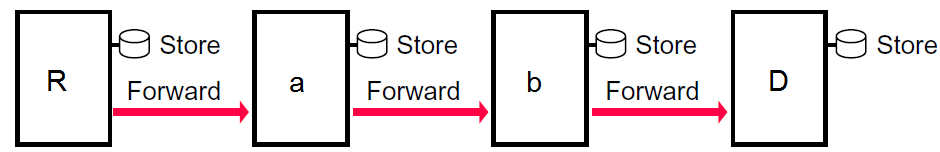
\includegraphics[width=0.9\textwidth]{figuras/cap_2/secao_1/armazena_envia.png}
\caption{Encaminhamento nas DTNs. Baseado em \cite{umrKehr}.}
\label{armazena_envia}
\end{figure}

A existência de dispositivos com hardware limitado torna importante o gerenciamento inteligente das mensagens acumuladas nos nós, pois, devido a limites de armazenamento, pode ser necessário excluir algumas em prol do armazenamento de outras. A mensagem que será apagada deve ser escolhida de forma a amenizar ocorrências de situações difíceis de prever, como apagar uma mensagem instantes antes de se encontrar com o destinatário.

Observa-se a importância dos contatos nas DTNs, pois a troca de mensagens só é possível na ocorrência dos mesmos. Como visto em \cite{rfc4838}, os contatos podem ser classificados de acordo com sua previsibilidade:

\begin{itemize}
    \item \textbf{Previsíveis:} Como o próprio nome indica, podem ser previstos de alguma forma. As redes espaciais são bons representantes para esta categoria devido ao fato de ser possível determinar, precisamente, o correto momento do envio e recepção de mensagens visto o comportamento cíclico dos astros;
    \item \textbf{Imprevisíveis:} São totalmente ou parcialmente estocásticos, ou seja, não é possível determinar, precisamente, quando e onde irão ocorrer. Redes onde os nós não possuem um padrão de comportamento bem definido representam esta categoria, sendo um exemplo as redes Ad Hoc.
\end{itemize}


Apesar de serem comumente encontradas na literatura como Redes Tolerantes a Atrasos e Desconexões, existem outras terminologias, tais como: Redes com Conectividade Eventual, Redes Desconectadas e Redes com Conectividade Transiente. Recentemente, o termo DTN também pode ser encontrado como Disruption-Tolerant Networking e é oriundo de atribuições realizadas pela DARPA, a Agência de Projetos de Pesquisa Avançada de Defesa dos Estados Unidos, que faz altos investimentos em pesquisas relacionadas às DTNs, principalmente para uso militar \cite{krishnan2007spindle, sehl2013viability}.

\newpage
\subsection{Arquitetura}

A definição de uma arquitetura básica capaz de atender e amenizar os problemas enfrentados nas DTNs é muito importante. Tal trabalho foi realizado por \cite{fall2003delay} e é alvo de inúmeros estudos e complementações. Em seu artigo, Fall propõe uma arquitetura baseada no armazenamento e reenvio de mensagens e utilização de \emph{gateways}, responsáveis por interconectar regiões\footnote{Regiões são definidas como áreas onde há uma maior homogeneidade entre as características dos nós.} de uma DTN.

Como visto em \cite{rfc5050} e \cite{umrKehr}, a troca de mensagens entre os nós é implementada, nas DTNs, por meio de um modelo em camadas baseado no modelo OSI, assim como a Internet. O principal diferencial entre o modelo das DTNs e o da Internet é a existência da \emph{Camada de Empacotamento} (do inglês "Bundle Layer"), ilustrada na Figura \ref{camadas_dtn}. Esta camada é responsável pelo armazenamento temporário de mensagens, gerenciamento do \emph{buffer} de armazenamento utilizado pelos nós e abstração da troca de mensagens pelas aplicações que rodam sobre DTNs.

\begin{figure}[htp!]
\centering
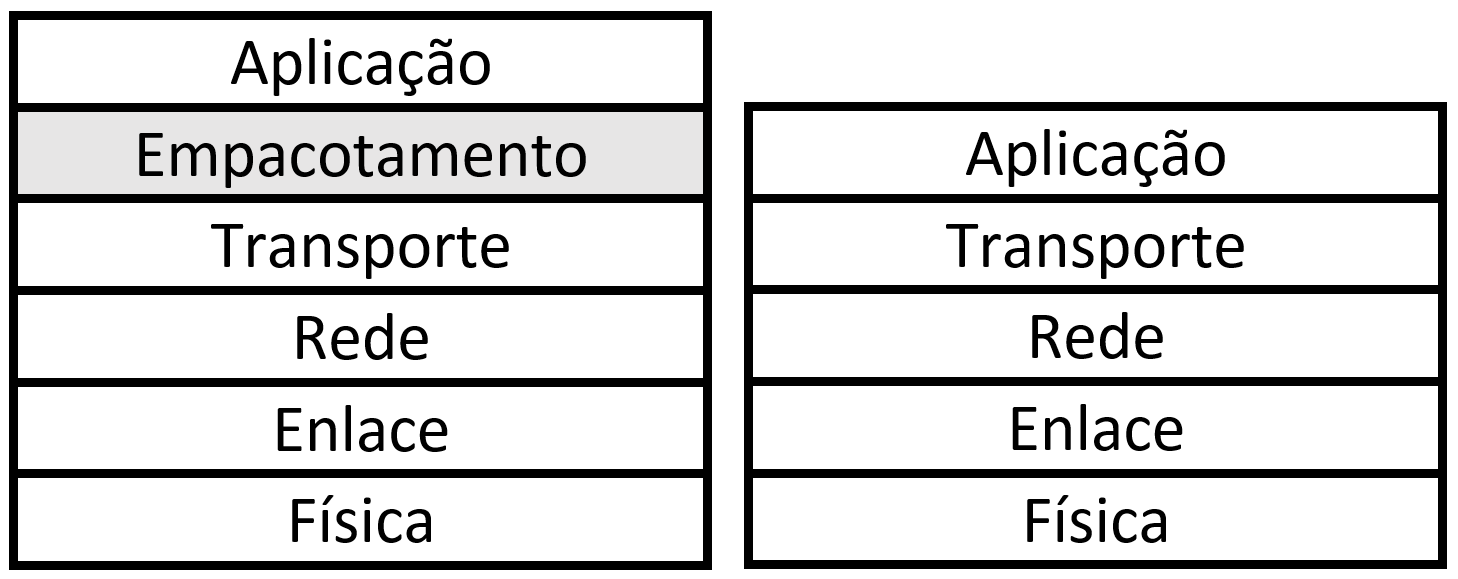
\includegraphics[width=0.7\textwidth]{figuras/cap_2/secao_1/camadas_dtn.PNG}
\caption{Pilha de camadas de comunicação das DTNs (esquerda) comparada com a da Internet (direita). Baseado em \cite{umrKehr}.}
\label{camadas_dtn}
\end{figure}

Os \emph{gateways} são dispositivos que compõem as DTNs capazes de armazenar e retransmitir mensagens utilizando diferentes protocolos de roteamento e transporte. Como exemplo, um \emph{gateway} pode receber uma mensagem de um nó utilizando os protocolos TCP e IP e retransmiti-la utilizando outros, como o SCTP e IP \cite{fall2003delay}. Seu uso se faz necessário pelo fato de DTNs de diferentes regiões executarem diferentes protocolos de comunicação, permitindo assim a interoperabilidade de protocolos existentes em arquiteturas distintas.

O modelo proposto por Fall prevê ainda o uso de tuplas para a identificação de objetos ou grupos deles. Elas possuem duas componentes. A primeira é responsável por identificar o nome de uma região e é estruturada de forma hierárquica e única. A segunda é responsável por identificar entidades ou grupo delas. Os \emph{gateways} ficam então responsáveis por armazenar tabelas de roteamento baseadas nessas tuplas, permitindo um mapeamento global, seja ele dinâmico ou estático, das regiões e otimização do redirecionamento das mensagens.

A Figura \ref{dtn_fall} ilustra a arquitetura proposta por Fall, onde existem quatro regiões (A, B, C e D) bem distintas, presença de diferentes dispositivos, identificados por tuplas, e meios de encaminhamento. O cenário apresentado é bastante diversificado, indo desde o transporte de mensagens por meio de um ônibus, identificado pela tupla \{B, R4\}, até a comunicação com um satélite artificial, identificado pela tupla \{D, Satellite\}.

\begin{figure}[htp!]
\centering
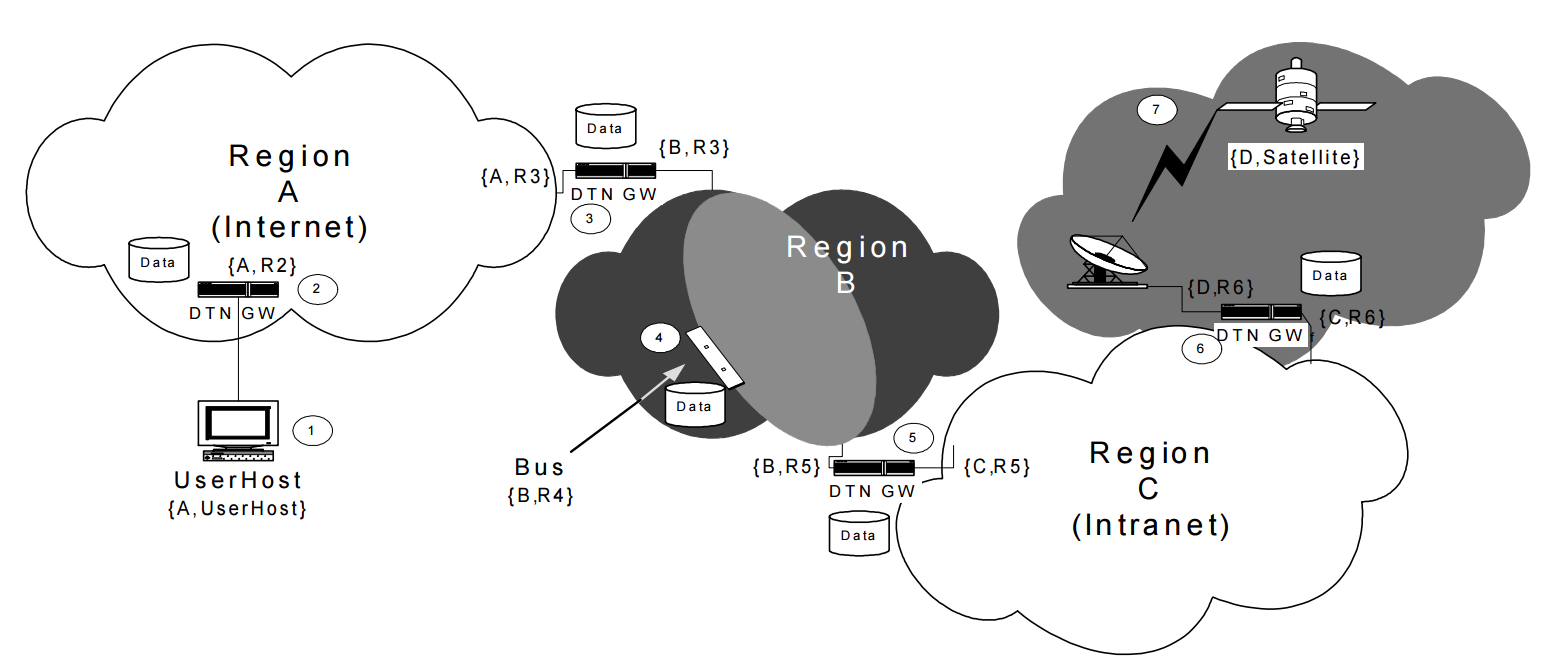
\includegraphics[width=1\textwidth]{figuras/cap_2/secao_1/dtn_fall.png}
\caption{Arquitetura de DTN utilizando gateways para interconectar DTNs com diferentes protocolos de comunicação \cite{fall2003delay}.}
\label{dtn_fall}
\end{figure}

O papel dos \emph{gateways} é reforçado na Figura \ref{dtn_fall}. Os \emph{gateways} identificados na região B como \{B, R3\} e \{B, R5\} armazenam temporariamente as mensagens enquanto o ônibus \{B, R4\} as transporta de um para o outro.

\subsection{Encaminhamento de Mensagens}
\label{subsec:encaminhamento_mensagens}
Protocolos de Encaminhamento de mensagens são importantes em qualquer arquitetura de redes de computadores. A partir deles as mensagens são comutadas nó a nó na rede até que elas sejam entregues aos seus destinos. Nas DTNs isso não é diferente e diversos protocolos de encaminhamento foram desenvolvidos voltados para as características dessas redes.

Os protocolos de encaminhamento destinados às DTNs podem ser divididos em dois grupos principais: Probabilísticos e Não-Probabilísticos. Cada grupo possui características próprias, como taxa de entregas de mensagens, taxa de utilização de buffers e controle da quantidade de cópias de mensagens existentes na rede.

\subsubsection{Protocolos Probabilísticos}

Protocolos Probabilísticos fazem uso de dados estatísticos calculados por meio de informações obtidas da própria rede, como taxa de encontro entre cada um dos nós, quantidade de retransmissões das mensagens, taxas de sucesso e insucesso das transmissões e quantidade de cópias existentes de uma determinada mensagem na rede. Esses protocolos utilizam critérios para determinar, a partir dos dados, os melhores critérios de encaminhamento a serem utilizados.

Por utilizarem dados estatísticos, os Protocolos Probabilísticos tendem a tomar melhores decisões de acordo com o reconhecimento da rede, pois a maior quantidade de dados obtida com o tempo melhora os dados estatísticos e, consequentemente, melhora as decisões.

Entre os Protocolos Probabilísticos, destaca-se o protocolo Prophet:

\begin{itemize}
    \item \textbf{Prophet:} De acordo com \cite{lindgren2003probabilistic}, este protocolo utiliza o histórico de encontros entre os dispositivos para a tomada de decisão de roteamento. Numa rede que utiliza este protocolo, cada um dos nós armazena uma lista com todos os nós que já foram encontrados e uma \emph{Previsibilidade de Entrega} que é calculada de acordo com a quantidade de encontros entre os nós e decai quando eles não entram em contato por um determinado tempo. Esse protocolo utiliza a propriedade da transitividade, pois se um determinado nó \emph{R} possui mensagens para um nó \emph{D} que ele nunca se encontrou, mas um nó intermediário \emph{I} se encontra constantemente com \emph{D}, para \emph{R} o nó \emph{I} terá maior relevância na propagação da mensagem do que um outro nó \emph{N} que nunca se encontrou com \emph{D};
    %\item \textbf{MaxProp \cite{burgess2006maxprop}:} Ainda sendo estudado.
\end{itemize}

\newpage

\subsubsection{Protocolos Não-Probabilísticos}

Protocolos Não-Probabilísticos caracterizam-se pela ausência do uso de dados estatísticos na retransmissão das mensagens, destacando-se os seguintes:

\begin{itemize}
    \item \textbf{Epidemic Routing:} Segundo \cite{vahdat2000epidemic}, este protoloco parte do pressuposto de que quanto mais cópias de uma mesma mensagem existirem na rede, maiores serão as chances de entrega. Numa rede que executa esse protocolo, os nós retransmitem todas as mensagens armazenadas em \emph{buffer} quando entram em contato com outro, inundando a rede com diversas cópias. Problemas como o congestionamento da rede e o estouro de \emph{buffers} são constantes, fazendo necessário o uso de técnicas para a redução desses problemas, como o uso de indicadores (\emph{beacons}) de entrega da mensagem, uso de políticas para priorizar umas em relação à outras (como o tempo de criação) e uso de um número máximo de saltos que uma mensagem pode sofrer;
    \item \textbf{Spray-and-wait:} Como visto em \cite{spyropoulos2005spray}, este protocolo foi desenvolvido com o intuito de reduzir a quantidade de duplicatas de uma mensagem na rede e as taxas de estouro de \emph{buffers} nos dispositivos. Basicamente, existem duas fases, uma de pulverização e outra de espera. Na fase de pulverização os nós vão disseminando a mensagem pela rede até que um número limitado de nós esteja armazenando a mensagem. Na fase de espera, os nós só retransmitem a mensagem quando o nó destino é encontrado. A mobilidade dos nós deve ser consideravelmente alta, pois nós pouco móveis podem acabar fazendo com que o destinatário nunca seja alcançado;
    \item \textbf{Direct Contact:} Em \cite{spyropoulos2007spray}, é visto que neste protocolo as mensagens só são retransmitidas se o remetente se encontra com o destinatário. Os problemas de congestionamento e estouro \emph{buffers} existente no protocolo epidêmico são praticamente resolvidos, mas as chances de entrega das mensagens são muito reduzidas, pois remetente e destinatário podem nunca se encontrar.
\end{itemize}

\subsubsection{Comparação entre os Protocolos Probabilísticos e Não-Probabilísticos}

Intuitivamente, percebe-se uma grande vantagem dos Protocolos Probabilísticos em relação aos Não-Probabilísticos.

Os Probabilísticos, com o uso de estatísticas provenientes da própria rede gerenciam de forma inteligente as retransmissões de mensagens, possuem baixas taxas de estouro de buffer, menor quantidade de duplicatas de mensagens e maiores taxas de entrega em relação aos Não-Probabilísticos. Sua característica adaptativa o torna mais eficiente de acordo com o tempo, mas, em redes recém implementadas, as probabilidades de erro e perdas de mensagens são elevadas.

Os protocolos Não-Probabilísticos baseiam-se primordialmente na mobilidade dos nós e em técnicas simples de roteamento de mensagens. Essas características os tornam problemáticos em redes com nós mais estáticos, mas de implementação simplificada em relação aos Probabilísticos. Mesmo aumentando as chances de entregas, a inundação da rede realizada pelo Protocolo Epidêmico pode acabar afogando os nós, fazendo com que o desempenho não seja satisfatório devido às altas taxas de estouro dos buffers.

\subsection{Aplicações Existentes}
\label{sec:aplicacoes}

Na literatura sobre DTNs inúmeros casos de aplicações são referenciados. Nesta subseção são apresentados alguns desses casos.

\subsubsection{O ZebraNet}

O projeto ZebraNet tem como objetivo monitorar a vida de zebras. Por meio de colares colocados nesses animais é feita a coleta e o armazenamento de dados referentes às suas vidas em seu habitat, permitindo uma análise detalhada do comportamento deles \cite{juang2002energy} \cite{zhang2004hardware}.

Assim como todo animal em seu ambiente natural, as zebras se movimentam de uma forma que a coleta de dados por humanos é dificultada, principalmente pelo fato de que os seres humanos afugentam esses animais. A solução para isso é obtida por meio do uso de colares que são colocados nas zebras e funcionam como nós de uma grande rede DTN. 

O encaminhamento das mensagens pelos dispositivos é feito de forma hierárquica. A posição dos nós dentro dessa hierarquia é baseada na quantidade de vezes que este se encontrou com a estação de coleta de dados. Quanto maior essa quantidade de encontros com a base, mais próximo do topo o nó estará da hierarquia. Estar próximo do topo significa que o nó tende a se encontrar muito com a base e, consequentemente, possui grande chance de se encontrar novamente num futuro próximo. A partir daí, quando um nó se encontra com dois dispositivos, um próximo do topo e outro distante, será dada a preferência de encaminhamento para o nó mais próximo do topo, visto que maiores são as chances dele se encontrar com a base num futuro próximo \cite{juang2002energy}.

A Figura \ref{zebra} apresenta uma zebra com o colar desenvolvido pelo projeto. Pode ser visto que ele foi desenvolvido para se adequar ao pescoço desses animais. Além disso, instalar esses dispositivos nesses animais exige que ele seja o mais confortável possível, visto que qualquer irritação gerada pelo mesmo pode influenciar nos resultados obtidos pelo projeto.

\begin{figure}[htp!]
    \centering
    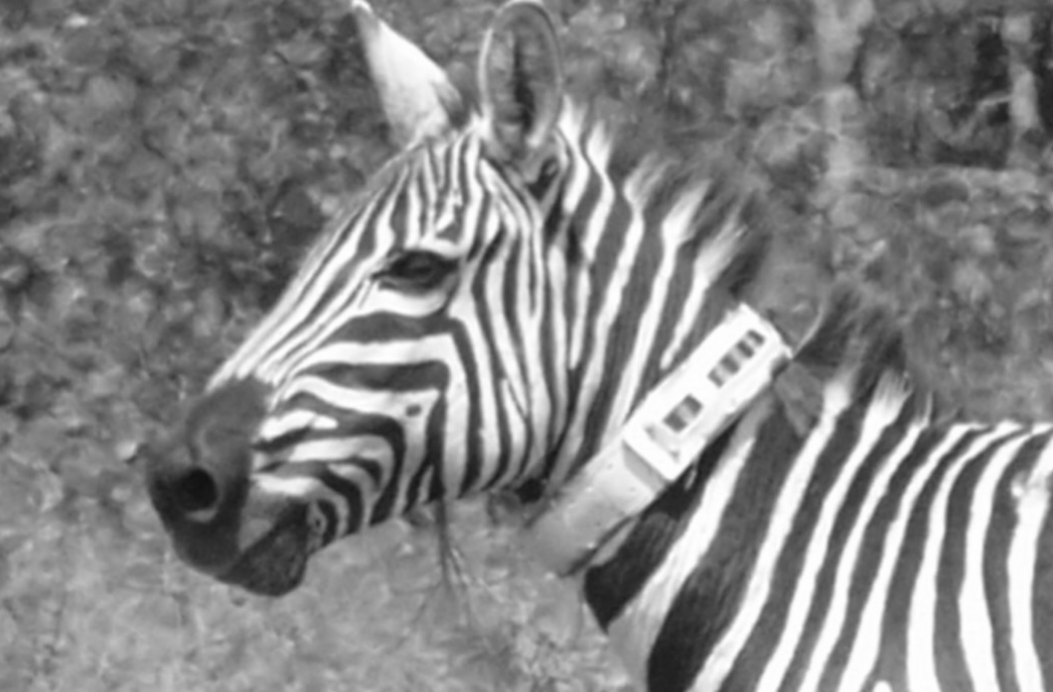
\includegraphics[width=0.8\textwidth]{figuras/cap_2/secao_1/zebranet.png}
    \caption{Zebra com o colar desenvolvido pelo projeto ZebraNet \cite{zhang2004hardware}.}
    \label{zebra}
\end{figure}

O estudo da vida das zebras por meio do ZebraNet trás contribuições para diversas áreas de estudo, como ecologia, biologia e redes de computadores.

\subsubsection{Redes Móveis Ad Hoc}

Um caso de aplicação das DTNs são as Redes Móveis Ad Hoc (do inglês "Mobile Ad Hoc Netwrok" ou MANET). Em geral, uma MANET, é uma infraestrutura autônoma composta por dispositivos móveis sem fio que trocam dados sem a necessidade de um elemento intermediador, como nas redes WiFi em modo Ad Hoc.

\subsubsection{O Wizzy Digital Courier}

Prover conectividade em áreas muito distantes de qualquer infraestrutura de Internet é um grande desafio e, já não é de hoje, que conectar regiões emergentes, como áreas rurais, atraem a atenção de pesquisadores \cite{tierProject}.

O Wizzy Digital Courier, nada mais é do que um projeto responsável por prover conectividade com a Internet por meio de uma DTN a escolas localizadas em locais remotos na África do Sul. Para isso, o projeto faz uso de uma motocicleta, equipada com dispositivos de armazenamento móveis, que realiza o encaminhamento dos dados até a cidade mais próxima que possui conexão com a Internet de alta capacidade. Geralmente, o processo de encaminhamento das mensagens com a motocicleta leva muitas horas, todavia é uma forma barata e acessível para os padrões econômicos da região. \cite{jain2004routing}


\subsubsection{Comunicação Espacial}

A comunicação entre satélites em órbita, estações, naves espaciais, sondas interplanetárias e telescópios depende da movimentação destes elementos e dos próprios movimentos dos corpos celestes, como planetas e estrelas. Os movimentos de rotação e translação dos planetas, estrelas e satélites naturais podem, eventualmente, gerar períodos de conexão e desconexão com centros localizados na Terra. A mobilidade e frequentes desconexões são características são típicas das DTNs e são marcantes neste cenário.

A Figura \ref{satelites} mostra um exemplo de sistema de comunicação interplanetária composto por dois satélites artificiais. Em um determinado instante \emph{a} do tempo, os satélites conseguem trocar dados pois não existem barreiras físicas suficientemente fortes para inviabilizar a comunicação. No instante \emph{b} a comunicação é inviabilizada pois o planeta marciano encontra-se entre os dois dispositivos.

\begin{figure}[htp!]
    \centering
    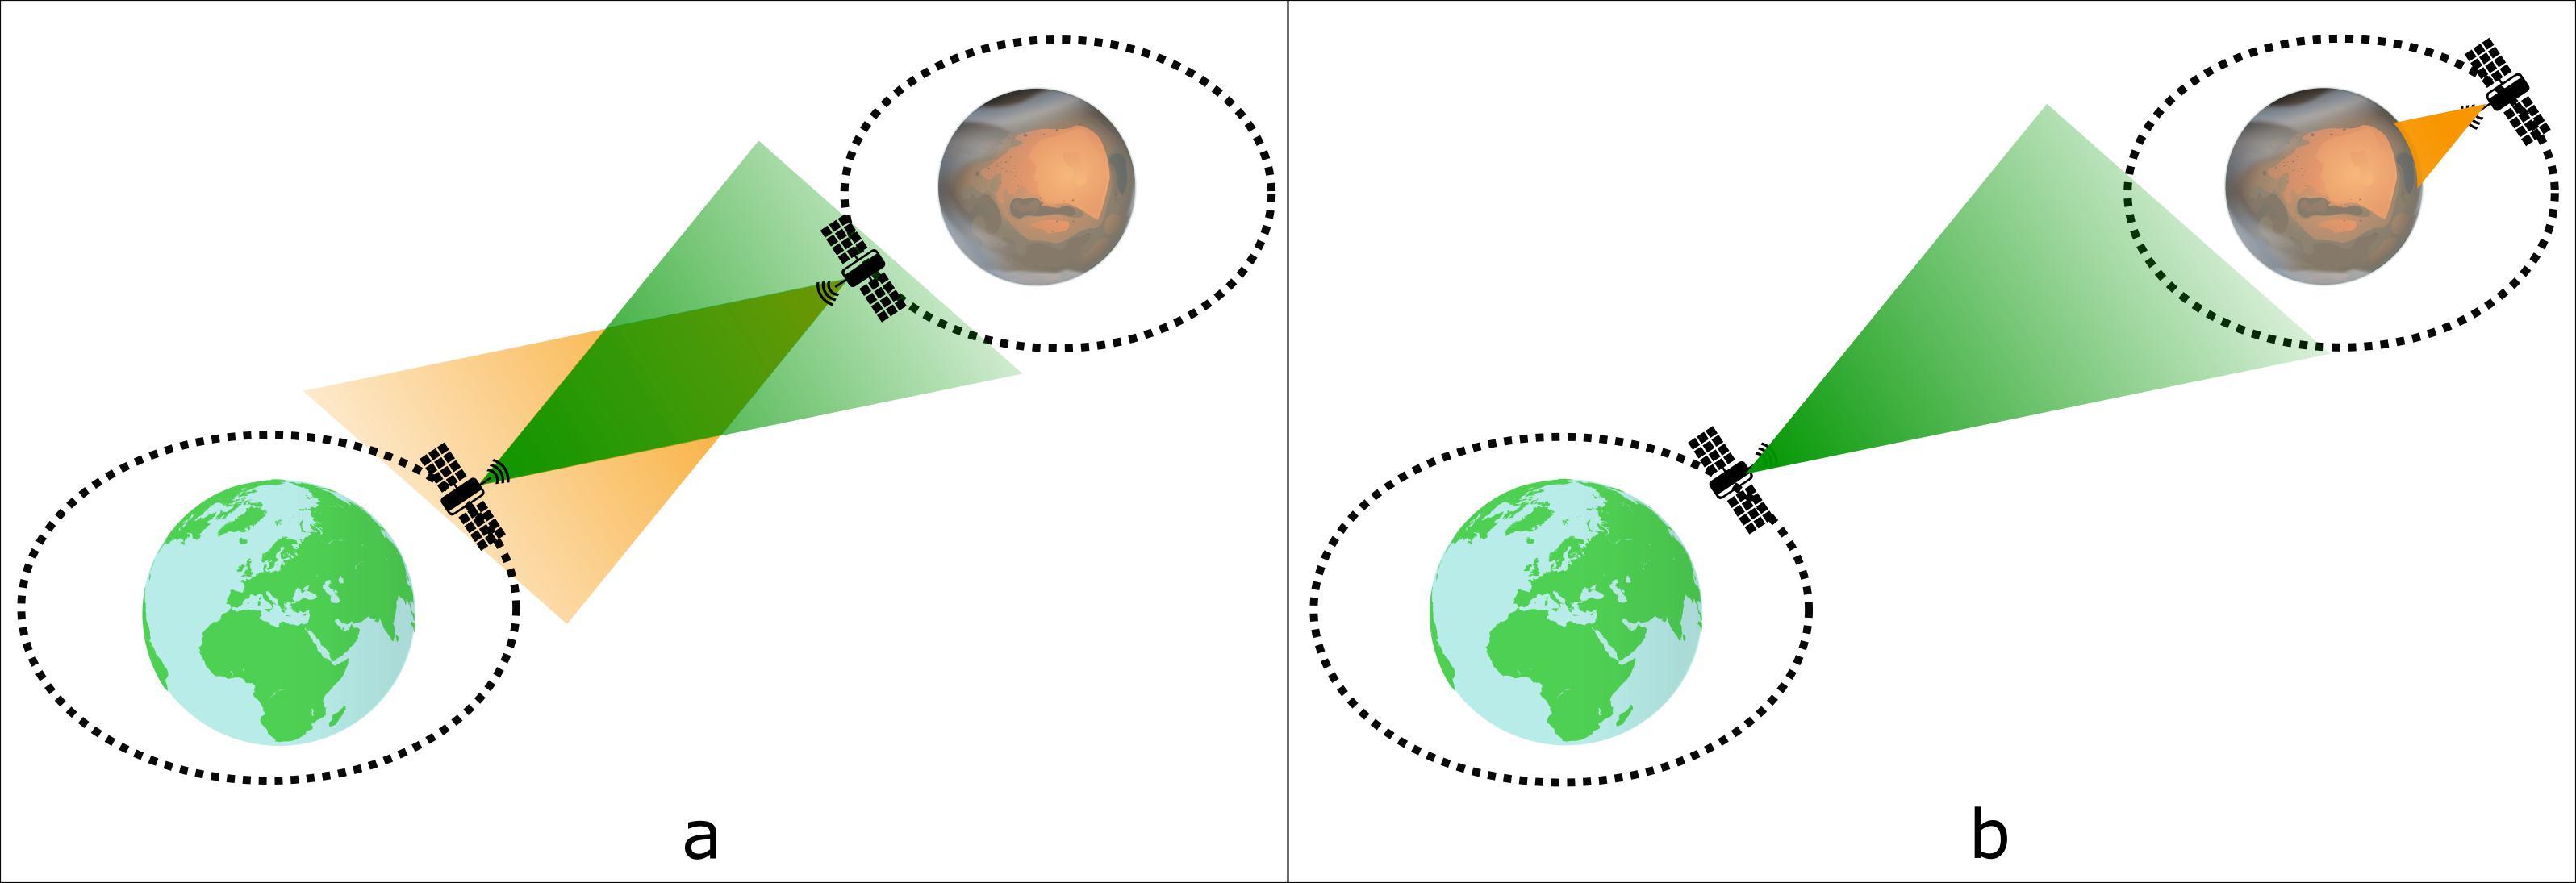
\includegraphics[width=1\textwidth]{figuras/cap_2/secao_1/satelites.png}
    \caption{Exemplo de comunicação espacial.}
    \label{satelites}
\end{figure}

\subsection{Principais Desafios}

As DTNs são conhecidas ainda como CHANTS ("Challenged NeTworks", ou "Redes com Desafios", em português) \cite{chen2006hybrid}. Tal atribuição remete, principalmente, a grande quantidade de desafios envolvidos na gerência e implementação de protocolos de roteamento para esse tipo de rede.

A característica móvel dos dispositivos torna necessário o uso de baterias que possuem capacidade de armazenamento de carga limitada. Essa limitação é um desafio inerente das DTNs e depende do uso de mecanismos de recarga e desenvolvimento de técnicas visando o consumo inteligente da energia por parte dos dispositivos.

O gerenciamento inteligente do consumo das baterias é, atualmente, alvo de grandes pesquisas, como pode ser visto em \cite{denis_artigo}. Silva, em seu artigo, realiza uma análise do consumo dos principais protocolos de roteamento das DTNs e, como principal resultado, afirma que a busca por dispositivos é grande responsável pelo consumo das baterias e aponta um intervalo ótimo de 32 segundos entre as buscas.

Em \cite{denis_artigo} não são considerados fatores como a probabilidade de contatos em regiões geográficas. A busca por dispositivos em áreas de maior quantidade de contatos registrada possui maior probabilidade de sucesso do que em áreas com menor quantidade, logo é de importante valia o estudo da dinamização do intervalo de busca proposto por Silva. Para tanto, podem ser utilizadas teorias relacionadas ao \emph{Referenciamento Geográfico} e \emph{Gradiente de Concentração} para o mapeamento da quantidade de contatos das regiões geográficas. Essas teorias são explanadas nas seções subsequentes.


\newpage
\section{Gradientes de Concentração}
\label{sec:gradientes_de_concentracao}

Nesta seção o conceito de Gradientes de Concentração é explanado por meio da contextualização e definição aceca deste tema. Após isso, é apresentada uma proposta de aplicação deste conceito na área de \emph{Redes Tolerantes a Atrasos e Desconexões}.

\subsection{Contexto}

Existem particularidades nas propriedades físico-químicas quando se trabalha com compostos. Intuitivamente, exemplifica-se que, ao se fazer uma bebida - um simples suco natural - é preciso realizar a mistura de determinados ingredientes, como água, açúcar e a polpa da fruta característica pelo tipo de suco.

O processo de mistura é, na maioria das vezes, tão simples que os indivíduos nem percebem ou não levam em consideração a complexidade envolvida. Isso se deve ao fato de ser simples do ponto de vista macroscópico. Partindo de um minúsculo ponto de vista, o molecular, as moléculas de água, portadoras de propriedades particulares, são capazes de interagir com os cristais de açúcar, dissolvendo-os até um ponto de equilíbrio, que se dá quando não é mais possível continuar esse processo, ou seja, não existem mais cristais, mas sim moléculas de sacarose\footnote{Substância extraída da cana-de-açúcar e beterraba, comum em produtos alimentícios, como adoçante de alimentos e bebidas, geleias, doces e, até mesmo, xaropes.} espalhadas pela água utilizada. 

A mistura de açúcar com água possui, inicialmente, uma heterogeneidade, existindo assim um \emph{Gradiente de Concentração}, ou seja, uma diferença de concentração (os cristais de açúcar possuem maiores concentrações de moléculas de sacarose do que a água pura) entre os elementos envolvidos, dando partida ao processo de dissolução dos cristais. Esse processo ocorre até um ponto que a mistura de água e açúcar se torne uniforme, ou homogênea, de forma que não exista mais um \emph{Gradiente de Concentração}.

\subsection{Definição}

Em química, o \emph{Gradiente de Concentração} indica a alteração no valor da concentração de determinada substância por unidade de espaço. Este conceito pode ser utilizado em diversas áreas, como física, biologia e geografia. Tal gradiente é, geralmente, representado de forma gráfica \cite{concentrationGradient}.

A mistura de água com açúcar caracteriza-se por uma situação semelhante a representada na Figura \ref{agua_acucar_copo} (onde as bolinhas vermelhas representam as moléculas de sacarose e, o fluido em azul, a água).

\begin{figure}[htp!]
\centering
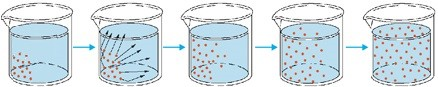
\includegraphics[width=0.80\textwidth]{figuras/cap_2/secao_2/agua_acucar_copo.jpg}
\caption{Difusão de moléculas de sacarose num copo de água \cite{concentrationGradient}.}
\label{agua_acucar_copo}
\end{figure}

É atribuído o nome \emph{difusão} ao processo representado na Figura \ref{agua_acucar_copo} \cite{concentrationGradient}. Não é objetivo deste trabalho explanar sobre as razões desse fenômeno. Em suma esse é um comportamento estocástico, natural e acontece a todo momento na natureza e no corpo humano.

Baseando-se em \cite{concentrationGradient}, é possível discretizar o processo de difusão da sacarose, obtendo o resultado visto na Figura \ref{modeculas_sacarose_agua}, onde a água pode ser vista na cor branca e as moléculas de sacarose na cor azul. É observada uma mistura gradativa do quadro esquerdo para o direita até que uma mistura quase perfeita seja alcançada.

A Figura \ref{gradiente_modeculas_sacarose_agua} apresenta os \emph{Gradientes de Concentração} para cada uma das etapas apresentadas na Figura \ref{modeculas_sacarose_agua}, baseado-se no material de \cite{concentrationGradient}. Nota-se, no gradiente à esquerda, uma grande concentração de substância na parte de baixo. A grande concentração ainda existe no gradiente do meio, mas a substância começou a se difundir para a parte superior. No último, a direita, há apenas uma cor uniforme, pois o gradiente já não existe mais, ou seja, as moléculas já se difundiram completamente.

\begin{figure}[htp!]
\centering
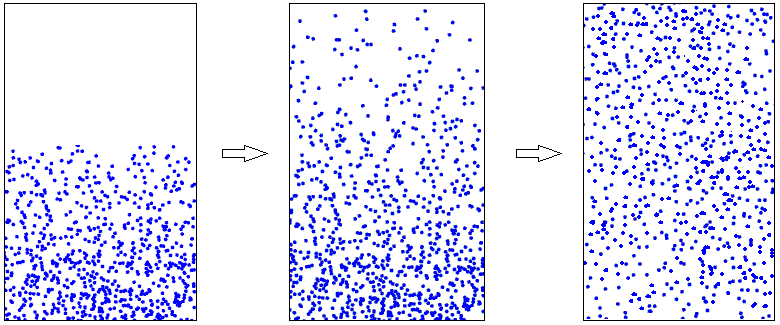
\includegraphics[width=1.0\textwidth]{figuras/cap_2/secao_2/modeculas_sacarose_agua.png}
\caption{Difusão de moléculas de sacarose num copo de água.}
\label{modeculas_sacarose_agua}
\end{figure}

\begin{figure}[htp!]
\centering
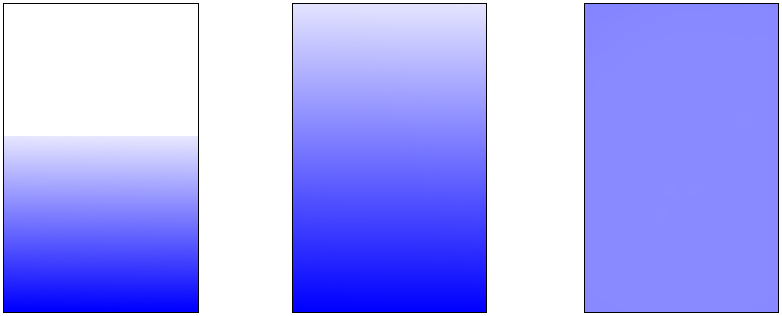
\includegraphics[width=1.0\textwidth]{figuras/cap_2/secao_2/gradiente_modeculas_sacarose_agua.png}
\caption{Gradientes de Concentração da difusão de moléculas de sacarose. A cor branca indica ausência de moléculas e, a cor azul intensa, alta concentração.}
\label{gradiente_modeculas_sacarose_agua}
\end{figure}
\newpage
\subsection{Aplicabilidade nas DTNs}

Na área de interesse deste trabalho, um \emph{Gradiente de Concentração} pode ser utilizado para representar dispositivos por unidade de área, permitindo representar regiões com muitos dispositivos como tendo maior concentração em relação a outras com menos dispositivos.

Os gradientes apresentados na Figura \ref{gradiente_modeculas_sacarose_agua} possuem uma única dimensão. Para o contexto geográfico, essa representação discretizada não traz resultados satisfatórios e, muito menos, intuitivos, principalmente pelo fato de que o mapeamento geográfico se basear em duas ou, até mesmo, três dimensões.

A Figura \ref{mapa_dispositivos} mostra um mapa com vários dispositivos distribuídos, representados por pontos verdes nomeados. Existe, no mapa, uma distribuição não uniforme de dispositivos, que é ainda mais evidenciada com a divisão em regiões de igual tamanho apresentada na Figura \ref{mapa_regioes_dispositivos}.

A concentração de dispositivos pode ser dada pela quantidade de nós de uma área dividida pela quantidade total de dispositivos da rede. A partir daí, é possível construir a Figura \ref{gradiente_mapa_regioes_dispositivos}, que representa um \emph{Gradiente de Concentração} bidimensional para o mapa inicialmente apresentado na Figura \ref{mapa_dispositivos}. A representação proporciona, de forma intuitiva, uma visualização discretizada de áreas com maior e menor incidência de dispositivos.

\begin{figure}[htp!]
\centering
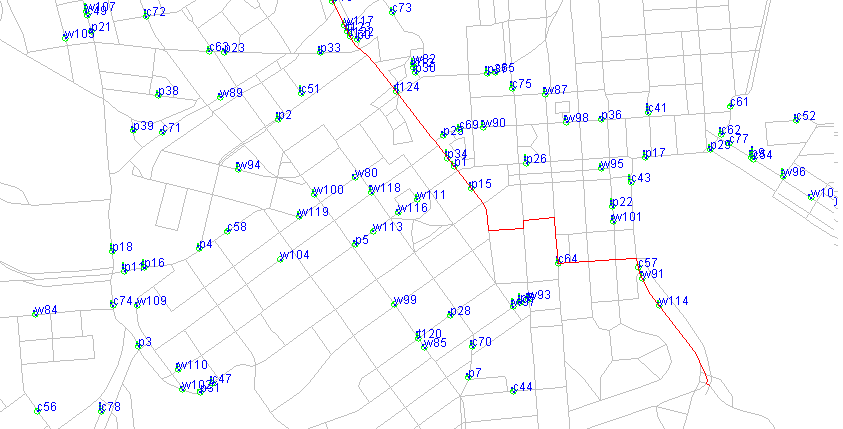
\includegraphics[width=1.0\textwidth]{figuras/cap_2/secao_2/mapa_dispositivos.png}
\caption{Mapa fictício com diversos dispositivos distribuídos por ele.}
\label{mapa_dispositivos}
\end{figure}

\begin{figure}[htp!]
\centering
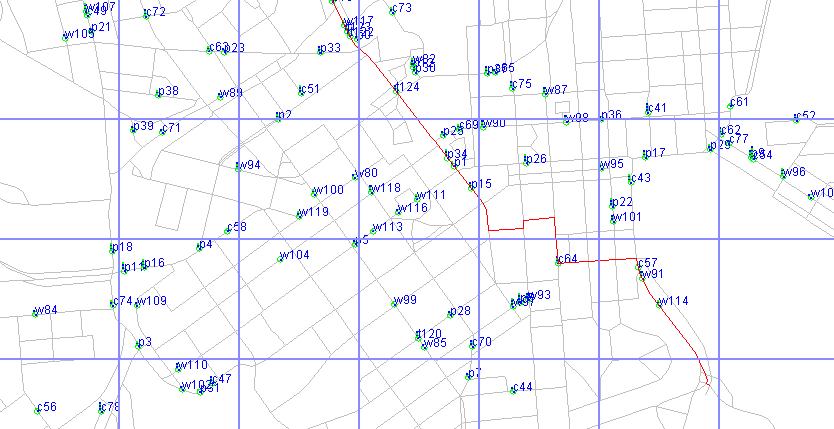
\includegraphics[width=1.0\textwidth]{figuras/cap_2/secao_2/mapa_regioes_dispositivos.png}
\caption{Mapa da Figura \ref{mapa_dispositivos} dividido em regiões de igual tamanho.}
\label{mapa_regioes_dispositivos}
\end{figure}

\begin{figure}[htp!]
\centering
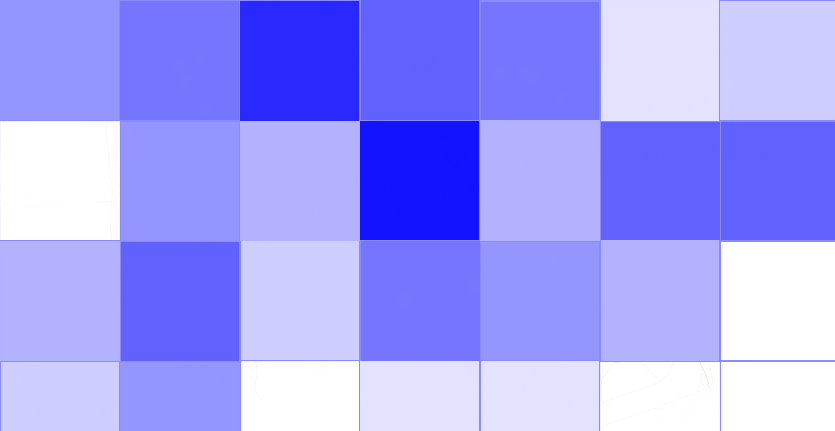
\includegraphics[width=1.0\textwidth]{figuras/cap_2/secao_2/gradiente_mapa_regioes_dispositivos.png}
\caption{Gradiente de Concentração baseado na Figura \ref{mapa_regioes_dispositivos}. A cor branca indica ausência de dispositivos e, a cor azul intensa, alta concentração.}
\label{gradiente_mapa_regioes_dispositivos}
\end{figure}

Cada região pode ser identificada e sua respectiva concentração definida por um número, inteiro ou real, responsável por indicar a intensidade desta, similar a cor. Quanto maior a concentração, maior este número e ainda maiores são as chances de encontrar algum dispositivo ao realizar uma busca. Portanto, pode-se reduzir ou aumentar a intensidade de buscas em determinadas áreas de acordo com a concentração, proporcionando um ajuste adaptativo de um importante fator no consumo de energia dos dispositivos: o intervalo de busca por dispositivos.

\subsection{Desafio}
\label{subsec:gradientes_desafios}
A representação da rede por meio de um gradiente tem como principal desafio a montagem do mesmo. O uso de técnicas de geolocalização são necessárias para o referenciamento e definição de regiões geográficas. Tais técnicas são detalhadas na Seção \ref{sec:GNSS}.

A construção do gradiente pode ser feita de forma independente entre os dispositivos que, ao entrarem em contato, trocam informações de seus gradientes numa forma semelhante a uma prosa: “Olha, eu sei que já ocorreram mais contatos na região X do que na Y, talvez isso possa ser útil para você.” e o outro responde “Legal. Como agradecimento, dar-lhe-ei as informações das regiões que já passei.”. 

Ao final de muitos contatos, os dispositivos terão um grande mapa das regiões onde eles já passaram tendo informações de localidades com maior e menor incidência de contatos, permitindo o ajuste dinâmico de fatores que influenciam no consumo de energia.

\section{Sistemas de Navegação por Satélites}
\label{sec:GNSS}
Nesta seção é apresentado o referencial teórico sobre Sistemas de Navegação por Satélites, seus princípios básicos, funcionamento e como podem ser aplicados no desenvolvimento da técnica adaptativa objetivada neste trabalho.

\subsection{Contexto e Definições}

A última década foi marcada pela popularização e evolução dos dispositivos móveis, principalmente os \emph{smartphones}. Esses dispositivos contam com diversas funcionalidades de software e hardware úteis para o dia a dia dos usuários, incluindo, em sua gigantesca maioria, serviços de geolocalização, que, por sua vez, dão ao usuário informações sobre a sua localização geográfica corrente.

Para o ser humano moderno, a possibilidade de saber qual a sua posição atual no mundo traz inúmeras vantagens que vão muito além de saber se está próximo de um estabelecimento que o mesmo está procurando para realizar as compras do mês. O acesso a essa informação traz a humanidade um leque de possibilidades, que são ainda mais ampliadas com o uso de uma rede de computadores. Como exemplo, podemos ter acesso à informações sobre o clima local, saber sobre os estabelecimentos próximos, calcular rotas precisas a partir da posição do usuário, associar o local a fotos e vídeos, e muito mais. Além disso, sistemas de georreferenciamento fazem o uso de imagens de satélites para determinar os limites de bairros e casas visando gerar informações de limites e posicionamento.

Existem, atualmente, dois principais Sistemas de Navegação por Satélites (do inglês "Global Navigation Satellite Systems" ou GNSS) funcionais responsáveis por permitir a descoberta de informações sobre o posicionamento de objetos no globo: O NAVSTAR-GPS (do inglês "Navigation Satellite with Time And Ranging Global Positioning System"), comumente conhecido apenas como GPS, e o GLONASS (sigla de origem russa para "Sistema de Navegação Global por Satélite"). 

%Ambos os sistemas necessitam do uso de receptores específicos, tornando obrigatório a existência de um hardware especial para cada um. \cite{vaz2013comparaccao}

\subsection{Referenciando a Posição de um Objeto no Globo}

Qualquer ponto na Terra pode ser referenciado por meio de um Sistema de Coordenadas Geográficas. De todos os modelos existentes o mais comum e prático é o baseado em linhas imaginárias conhecidas como \emph{meridianos} e \emph{paralelos}. Os meridianos cortam o globo do polo geográfico norte ao polo geográfico sul, já os paralelos são linhas ortogonais\footnote{Linhas que formam um ângulo de 90º ao se cruzarem.} aos meridianos. De todos os paralelos e meridianos que podem ser traçados na terra, destacam-se o Meridiano de Greenwich, que divide a terra em um lado ocidental e outro oriental, e o Paralelo da Linha do Equador, que divide a terra em polo sul e polo norte. \cite{fitz2008geoprocessamento}

\begin{figure}[htp!]
\centering
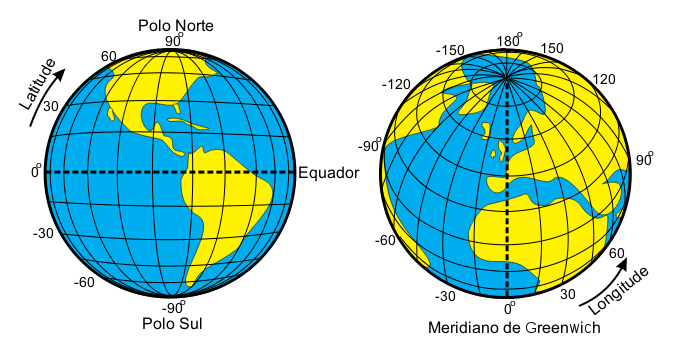
\includegraphics[width=0.80\textwidth]{figuras/cap_2/secao_3/latitude_longitude.png}
\caption{Latitude e Longitude}
\label{latitudeLingitude}
\end{figure}

A distância de qualquer ponto até a Linha do Equador é chamada de latitude e é medida em graus e varia de 0 a 90 graus, tanto para o norte (N) quanto para o sul (S). Para determinar a latitude de um ponto no globo, é preciso calcular o ângulo formado entre a linha do equador e uma reta que passa pelo ponto desejado e pelo centro da terra. Caso o ponto esteja em cima da linha do equador, não teremos a formação de um ângulo e, portanto, ele está na latitude 0º. \cite{fitz2008geoprocessamento}

Infelizmente, apenas com a latitude, não é possível determinar a posição exata de um ponto no globo. Para resolver isso é utilizada uma outra medida, a longitude. Esta medida, por sua vez, representa a distância do ponto desejado até o Meridiano de Greenwich e é calculada de forma similar a realizada para latitude, mas varia de 0 a 180 graus para leste (E) e para oeste (W). Um ponto que se localiza em cima do Meridiano de Greenwich está na longitude de 0º. \cite{fitz2008geoprocessamento}

A Figura \ref{washingtonDC} apresenta a latitude e a longitude aproximada de Washington D.C., a capital dos Estados Unidos da América.

\begin{figure}[htp!]
\centering
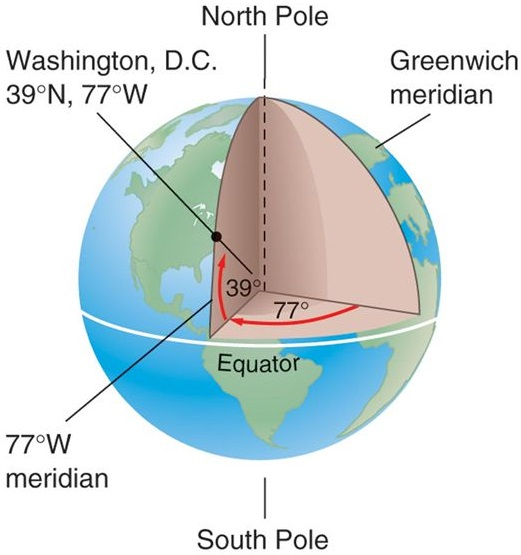
\includegraphics[width=0.60\textwidth]{figuras/cap_2/secao_3/washingtonDC.jpg}
\caption{Latitude e Longitude de Washington D.C.}
\label{washingtonDC}
\end{figure}

A distância em quilômetros de um grau a outro, que na latitude equivale a 111,12km e na longitude varia de 0 a 111,12km, torna necessário o uso de valores com várias casas decimais para representar com exatidão a posição de um objeto no globo. Para efeitos de simplificação, existe um modelo onde cada grau é dividido em duas componentes, uma de minutos (') e outra de segundos ("). Cada grau possui 60 minutos e cada minuto possui 60 segundos \cite{fitz2008geoprocessamento}. 

A divisão da latitude e da longitude em componentes torna possível simplificar a fala de uma coordenada geográfica. Como exemplo, a posição geográfica da \emph{Universidade Vila Velha} se dá na latitude 20.354043ºS e na longitude 40.299163ºW, que, quando convertido para o modelo utilizando minutos e segundos, se torna \newline 20º21'14,6"S e 40º17'57"W, respectivamente. A pronúncia do sistema em minutos e segundos é mais fácil de ser entendida e associada, pois discretiza os valores decimais muito longos que seriam necessários para referenciar um ponto no globo.

\subsection{O NAVSTAR-GPS}

O NAVSTAR-GPS, ou apenas GPS, como já foi introduzido, é uma tecnologia utilizada para determinar a posição geográfica de dispositivos no globo terrestre, fazendo uso de satélites artificiais, que funcionam como pontos de referência no espaço de posição muito bem conhecida. Além disso, foi desenvolvido pelo Departamento de Defesa dos Estados Unidos, o DOS (do inglês "Department of Defense"), está operacional desde 1994 e, devido ao tempo de operação, é mais popular em relação ao GLONASS.

A concepção do GPS permite que qualquer usuário situado na superfície terrestre, ou próximo dela, tenha a sua disposição, pelo menos, quatro satélites artificiais para serem rastreados, permitindo o conhecimento em tempo real da sua posição e uso sob condições climáticas extremas \cite{miguens1996navegaccao}. O GPS é um sistema passivo, pois não necessita que o usuário envie informações para os satélites, ficando estes responsáveis pelo envio dos sinais necessários.

Para calcular a posição de um usuário com precisão é utilizado um sistema de triangulação que faz uso da posição de três satélites e as suas respectivas distâncias até um receptor em terra. A distância do receptor até o satélite pode ser obtida por meio da medição do intervalo de tempo decorrido entre a transmissão dos sinais pelos satélites e a recepção pelo dispositivo receptor, sendo ela utilizada como raio de uma esfera cujo centro é a posição do satélite. A posição do usuário é o ponto em comum de interseção das três esferas, como ilustrado na Figura \ref{triangulacao_gps}.

\begin{figure}[htp!]
\centering
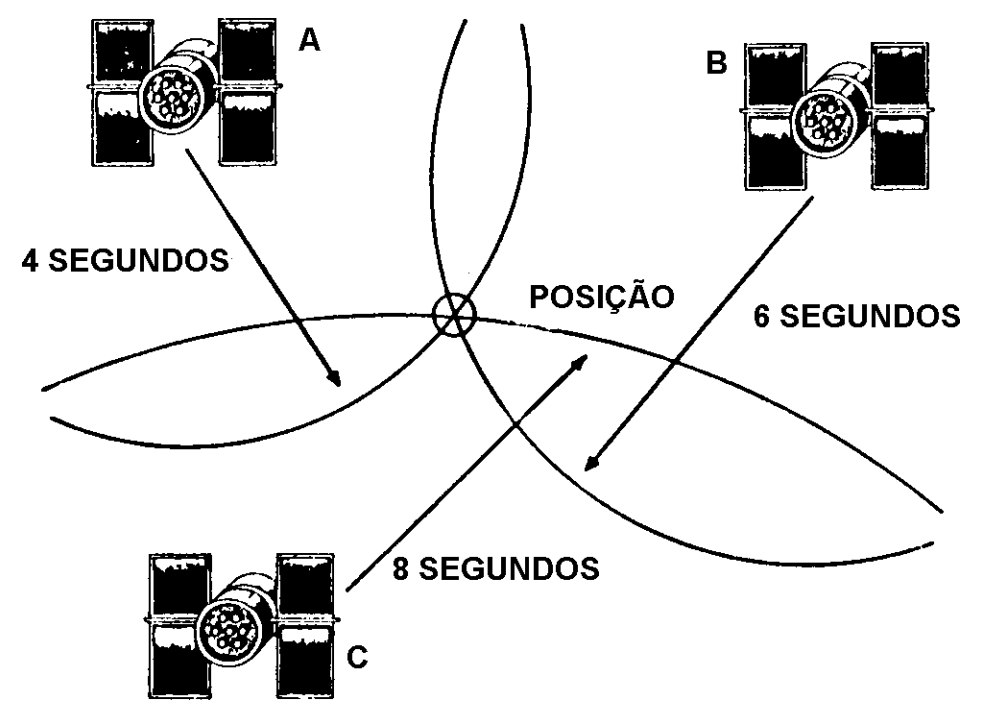
\includegraphics[width=0.60\textwidth]{figuras/cap_2/secao_3/triangulacao_gps.png}
\caption{Sistema de triangulação utilizado pelo NAVSTAR-GPS \cite{miguens1996navegaccao}.}
\label{triangulacao_gps}
\end{figure}

O cálculo do tempo decorrido entre a emissão do sinal e a recepção no dispositivo utilizado não é tão simples, pois exige a perfeita sincronização do relógio de todos os elementos envolvidos. Em situações práticas isso é muito improvável de acontecer e faz necessário o uso de mais um satélite para o processo, daí vê-se a importância da disponibilidade de, pelo menos, quatro satélites.

Não é objetivo deste trabalho realizar explanações muito específicas sobre o funcionamento do GPS. Detalhes de hardware, software e conceitos mais específicos podem ser encontrados em \cite{longley2009sistemas}.

\subsection{O GLONASS}

O GLONASS é uma tecnologia georreferenciamento de origem russa e, assim como o GPS, foi desenvolvido inicialmente para uso militar. Esse sistema só pôde ser considerado operacional em nível mundial no final 2011 e, a partir daí, começou lentamente a ser acoplado aos smartphones \cite{vaz2013comparaccao}, principalmente após o governo russo ter criado barreiras de importação para dispositivos que suportem apenas a tecnologia norte americana \cite{impostoRussia}.

O funcionamento da tecnologia russa é semelhante ao do GPS visto na Figura \ref{triangulacao_gps} e tem se tornado cada vez mais popular no mercado de dispositivos móveis e possui uma precisão muito próxima ao GPS \cite{vaz2013comparaccao}.

Até o ano de 2011, GPS e GLONASS eram totalmente incompatíveis entre-si, pois utilizavam técnicas de modulação e frequências diferentes. Entretanto, foi nesse ano que o GLONASS-K foi lançado e, por sua vez, possibilitou que dispositivos operem com as duas tecnologias utilizando um único receptor, visto que ele trabalha com frequências e modulações semelhante aos da tecnologia americana\newline \cite{kovar2011interoperable}.

\subsection{Contribuição para as Redes Tolerantes a Atrasos}

A descoberta da posição geográfica de dispositivos contribui de forma significativa em diversas áreas de pesquisa, entre elas as Redes Tolerantes a Atrasos. Conhecer a posição de cada um dos dispositivos que compõem uma DTN permite o levantamento de estatísticas de contatos ocorridos entre dispositivos em regiões preestabelecidas, abrindo mão para o gerenciamento inteligente de parâmetros que influenciam no consumo de energia dos dispositivos envolvidos.

A concentração pode ser calculada por meio da relação entre a quantidade total de contatos registrados e a quantidade de contatos ocorridos na região onde um nó se encontra. Quanto maior a concentração, maiores as chances de um dispositivo encontrar outro ao realizar uma busca e, portanto, é mais inteligente aumentar o consumo visando usufruir das oportunidades previstas. Quanto menor a concentração, menores as chances de encontrar outro dispositivo e, consequentemente, é mais inteligente economizar energia para momentos oportunos.

É importante ressaltar que o conceito de regiões apresentado na Seção \ref{sec:DTN} é diferente do que é utilizado para regiões geográficas. O primeiro refere-se a características relacionadas a protocolos, por exemplo, e aqui refere-se áreas geográficas.

\subsection{Consumo de Energia em Dispositivos Móveis}
\label{subsec:consumo_gps}
Visando o aumento da quantidade de mensagens entregues, é inerente no âmbito das DTNs tornar inteligente o consumo energético dos dispositivos. Isso implica numa análise do uso das baterias pelos dispositivos de GNSS quando considerada a contribuição proposta na Subseção anterior.

Em \cite{carroll2010analysis} foi realizado um estudo do consumo energético de diversos componentes existentes em smartphones, tais como CPU, memória RAM, memórias de armazenamento, além, é claro, de dispositivos de GPS, utilizando para isso técnicas e equipamentos de medição adequados.

Relativo ao consumo de dispositivos GPS, Carroll indica que, quando habilitados, eles consomem 143,1mW utilizando uma antena interna e 166,1mW quando utiliza-se uma antena externa. Ainda é explicitado no trabalho de Carroll que, quando desabilitados, os dispositivos GPS não realizam qualquer consumo de energia.

Outro resultado relevante apontado por Carroll é o de que não existem diferenças de consumo quando a quantidade de satélites visíveis é analisada. Sendo assim, é possível concluir que seus resultados podem ser utilizados em simulações sem a necessidade de simular a movimentação de satélites para aumentar o grau de realismo.

É visto que o estudo de Carroll é de importante valia na simulação da técnica desenvolvida neste trabalho, visto que ela baseia-se no uso de dispositivos de Georreferenciamento. Além disso, o trabalho referenciado permite aumentar o grau de realismo das simulações realizadas no que diz respeito ao consumo de energia. 

Para efeitos de simplificação, as simulações realizadas no capítulo \ref{cap:testes} consideram a média dos consumos apontados por Carrol, ou seja, 154,6mW.

\section{Conclusão do Capítulo}\label{sec:conclusao_cap_2}

A primeira seção deste capítulo apresentou um breve estudo sobre as DTNs, incluindo conceitos relacionados, arquitetura, aplicações e uma análise sobre o problema de energia existente. Além disso, ainda sobre as DTNs, os principais protocolos de disseminação foram descritos de forma sucinta.

Conceitos relacionados aos Gradientes de Concentração foram apresentados na seção subsequente a das DTNs. A explanação intuitiva foi utilizada visando facilitar o entendimento da analogia utilizada para a aplicação no ambiente das redes objetivadas neste trabalho.

Foi visto que o estudo e dinamização do intervalo de busca proposto por \newline \cite{denis_artigo} pode ser realizado a partir da análise da incidência de contatos em regiões previamente estabelecidas. Para tanto, foram apresentados conceitos sobre referenciamento geográfico, descrevendo sucintamente como referenciar posições no globo e as principais tecnologias de referenciamento existentes atualmente.

A importância da análise incremental apresentada neste capítulo se dá pelo principal problema existente nas DTNs: o consumo de energia. Não existem, atualmente, formas de solucioná-lo definitivamente, mas é possível desenvolver técnicas de software que visam realiza o consumo inteligente das baterias, que é o principal objetivo do presente trabalho.

%capítulo 3 - Tecnologias Utilizadas
\chapter{TECNOLOGIAS UTILIZADAS} \label{cap:theONE}

É objetivo deste capítulo descrever as tecnologias utilizadas para a elaboração da técnica objetivada neste trabalho.

Inicialmente é apresentado o simulador The ONE, responsável por permitir implementação e teste da técnica elaborada utilizando, para tanto a plataforma Java. Para tanto, as principais características do simulador são abordadas, tendo com foco a descrição da arquitetura modular do simulador.

Após a apresentação do simulador The ONE, a plataforma Java é brevemente abordada e, em seguida, é apresentada a ferramenta Gnuplot, responsável pela geração dos gráficos de apresentação dos resultados obtidos no capítulo \ref{cap:testes}.

Ao final do capítulo, é apresentada a conclusão, onde é realizado fechamento deste capítulo.

\section{Simulador The ONE}\label{sec:theONE}

O \emph{The Opportunistic Network Environment Simulator}, ou apenas The ONE, é uma ferramenta open source modular construída utilizando a plataforma Java e que permite a simulação de DTNs e implementa os principais mecanismos necessários para funcionamento dessas redes, como algoritmos de disseminação e gerenciamento de mensagens \cite{keranen2009one}. A Figura \ref{theONE} apresenta os módulos do simulador e os seus respectivos relacionamentos. 

Quanto a sua utilização, o The ONE baseia-se na definição de um cenário de simulação onde é possível configurar diversos elementos, como eventos, protocolos de encaminhamento, modelos de movimentação, características dos dispositivos e relatórios a serem gerados. Tais itens são melhor detalhados nas subseções a seguir, começando pelo Encaminhamento de Mensagens, passando pelo Módulo de Energia, Modelos de Movimento, Eventos, Relatórios e Automação de Testes, Dispositivos e, finalmente, uma breve apresentação da Interface Gráfica do mesmo.

\begin{figure}[htp!]
    \centering
    \includegraphics[width=1\textwidth]{figuras/cap_3/secao_1/TheONEArchtecture.png}
    \caption{Arquitetura do simulador The ONE \cite{keranen2009one}.}
    \label{theONE}
\end{figure}

\subsection{Encaminhamento de Mensagens}

O simulador The ONE nativamente é compatível com os principais protocolos de encaminhamento existentes em DTNs. Destacando-se os protocolos Prophet, Epidemic Routing, Spray-and-Wait e Direct Contact, que foram explanados na subseção \ref{subsec:encaminhamento_mensagens}. Todos os protocolos são implementados junto ao módulo \emph{routing} exibido na Figura \ref{theONE}.

A arquitetura modular do simulador possibilita grande flexibilidade quando deseja-se testar novos protocolos, bastando para tanto implementar o modelo desejado e integrá-lo ao módulo \emph{routing}. Para isso, o desenvolvedor do novo protocolo a ser testado precisa apenas herdar e sobrescrever, caso necessário, as características da classe \emph{ActiveRouter}, que, por sua vez, define operações básicas comuns de todos os protocolos de encaminhamento voltado para as DTNs, como decisões estratégicas de envio e recepção de mensagens e o gerenciamento do buffer de mensagens.

Quanto à simulação dos protocolos, um dos principais diferenciais do simulador escolhido é a possibilidade de definir grupos de nós, onde, cada grupo, pode executar diferentes protocolos de encaminhamento e possuir detalhes de hardware únicos, como tamanho dos buffers de armazenamento e antenas de rádio com diferentes capacidades.

\subsection{Módulo de Energia}
\label{modulo_energia}
Integrado ao módulo \emph{Routing}, há o módulo \emph{Energy Model}, que é responsável por realizar a simulação das baterias e do seu respectivo consumo. Esse módulo foi implementado por \cite{denis_artigo} e foi integrado oficialmente ao simulador The ONE na sua última versão, a 1.6, lançada em 7 de outubro de 2015 \cite{theOne_github}.

O módulo de energia desenvolvido por \cite{denis_artigo} considera que todos os dispositivos possuem cinco estados básicos de funcionamento:

\begin{itemize}
    \item \textbf{Desligado:} Neste estado, o nó não pode fazer uso de suas interfaces de rede, seja por falta de energia ou por uma decisão feita pelo protocolo de encaminhamento, como por exemplo economizar energia durante algum tempo. Além disso, não é possível estabelecer conexões com outros nós e, como consequência, não pode enviar e receber mensagens;
    \item \textbf{Inativo:} O nó, neste estado, tem as suas interfaces de rede ligadas mas está adormecido. Todavia, pode ser detectado e contatado por outros nós. Numa situação real este estado é responsável pelo consumo muito pequeno de energia, porém ele não é considerado por parte deste módulo;
    \item \textbf{Buscando:} Neste estado o nó encontra-se na procura por nós vizinhos para que possa estabelecer contato e, posteriormente, receber e enviar mensagens. Em suma, os nós entram periodicamente neste estado de acordo com o intervalo de busca pré-definido;
    \item \textbf{Transmitindo:} Estado onde o nó envia mensagens para outro;
    \item \textbf{Recebendo:} Estado onde o nó está recebendo mensagens de outro.
\end{itemize}

De acordo com \cite{denis_artigo}, é a partir do estado que o nó se encontra que o controle do consumo energia é realizado. Quando o nó tem sua interface no estado Inativo não é considerado o consumo de energia. Entretanto, quando o nó encntra-se apto para efetuar operações de busca por outros nós, envio e recebimento de mensagens o consumo é considerado de acordo com as propriedades definidas. Ao realizar uma operação de busca por outros nós, o módulo calcula a quantidade de energia consumida e decrementa da quantidade atual por meio do método \emph{reduceEnergy}. Quando se trata das operações de envio e recepção de mensagens, o módulo opera de forma um pouco diferente, pois decrementa a quantidade de energia definida a cada segundo de duração da operação de envio ou recebimento.

\subsection{Modelos de Movimento}

Os modelos de movimentação são responsáveis por descrever como será o deslocamento dos nós dentro da rede e são suportados diversos deles pelo módulo \emph{Movement Models}. O simulador apresenta nativamente o suporte a dois principais tipos de modelos de movimentação: sintéticos ou capturados de uma DTN real.

Os modelos sintéticos caracterizam-se por gerarem, seja aleatoriamente ou não, o caminho que os nós realizam no ambiente simulado. Podendo, para tanto, serem definidos mapas por onde nós podem se movimentar. Já os modelos capturados, são caracterizados por serem obtidos de uma DTN real e convertidos para o padrão de representação do simulador que, a partir daí, define o padrão de comportamento dos nós como o sendo do ambiente real.

Capturar a movimentação de nós num ambiente real e utilizá-los dentro de um ambiente simulado permite verificar como a rede pode se comportar quando são utilizados protocolos diferentes dos que estão em operação no ambiente real, além, é claro, de permitir maior grau de realismo nas simulações.

\subsection{Eventos}

Os eventos, gerados e processados pelo módulo \emph{Event Generators}, nada mais são que as mensagens trocadas entre nós da rede simulada. As mensagens são sempre "de um para um", ou seja, são originadas em um nó específico e destinadas a outro nó específico.

O simulador permite que sejam configurados parâmetros como o intervalo de tempo que um dispositivo gera mensagens para outro além do tamanho das mesmas. Pode-se, é claro, definir para ambos os parâmetros um valor mínimo e máximo, ficando o simulador responsável por gerar valores aleatórios dentro do intervalo definido.

\subsection{Relatórios e Automação de Testes}

Dentre todas as funcionalidades já apresentadas destaca-se a geração de relatórios pelo módulo \emph{Visualization and Results} e a possibilidade de automatização de testes implementada pelo módulo principal \emph{Simulation Engine}. 

A geração de relatórios têm sua importância destacada diante da necessidade de avaliar o comportamento da rede diante de parâmetros definidos e, muito além disso, testar novas técnicas implementadas dentro do simulador. Existem diversos relatórios disponíveis, destacando-se para utilização neste trabalho os seguintes:

\begin{itemize}
    \item \textbf{MessageDeliveryReport:} Este relatório detalha com alta granularidade a quantidade acumulada de mensagens entregues e geradas, além da probabilidade de entrega de mensagens da rede de acordo com o tempo de simulação;
    \item \textbf{EnergyLevelReport:} Tendo sido desenvolvido por \cite{denis_artigo}, este relatório detalha a quantidade de energia contida nas baterias de cada um dos dispositivos de acordo com o tempo de simulação, possibilitando o cálculo da linha de tendência de consumo e a quantidade média de energia armazenada nas baterias.
\end{itemize}

Quanto a automação dos testes, o simulador permite programação de testes por meio de arquivos de configuração e a sua execução a partir da linha de comando em modo batch. A cada teste realizado o simulador gera os respectivos relatórios de teste para que possam ser analisados a fundo posteriormente.

\subsection{Dispositivos}

O simulador The ONE permite configurar grupos de nós, onde, cada um deles, possui uma determinada quantidade de dispositivos com características específicas, como velocidade de movimentação, modelo de movimento, interfaces de rede e capacidade das baterias. Quanto às interfaces de rede, é possível configurar a distância máxima de alcance do sinal de rádio e a velocidade máxima que ela pode operar.

A possibilidade de criar grupos com diversas características únicas permite verificar a interoperabilidade entre os protocolos de encaminhamento, além de simular o comportamento da rede quanto a existência de nós com características distintas.

\subsection{Interface Gráfica}

O simulador permite a visualização em tempo real da simulação por meio de sua interface gráfica, apresentada na Figura \ref{interface_theONE}.  É possível acompanhar individualmente a movimentação dos nós, o estado (ligado/desligado), alcance das interfaces, situação dos buffers e o estado das conexões (up/down/relay). A Figura \ref{node_theONE} apresenta os detalhes individuais do nó \emph{p28} durante uma simulação realizada utilizando o The ONE.

\begin{figure}[htp!]
    \centering
    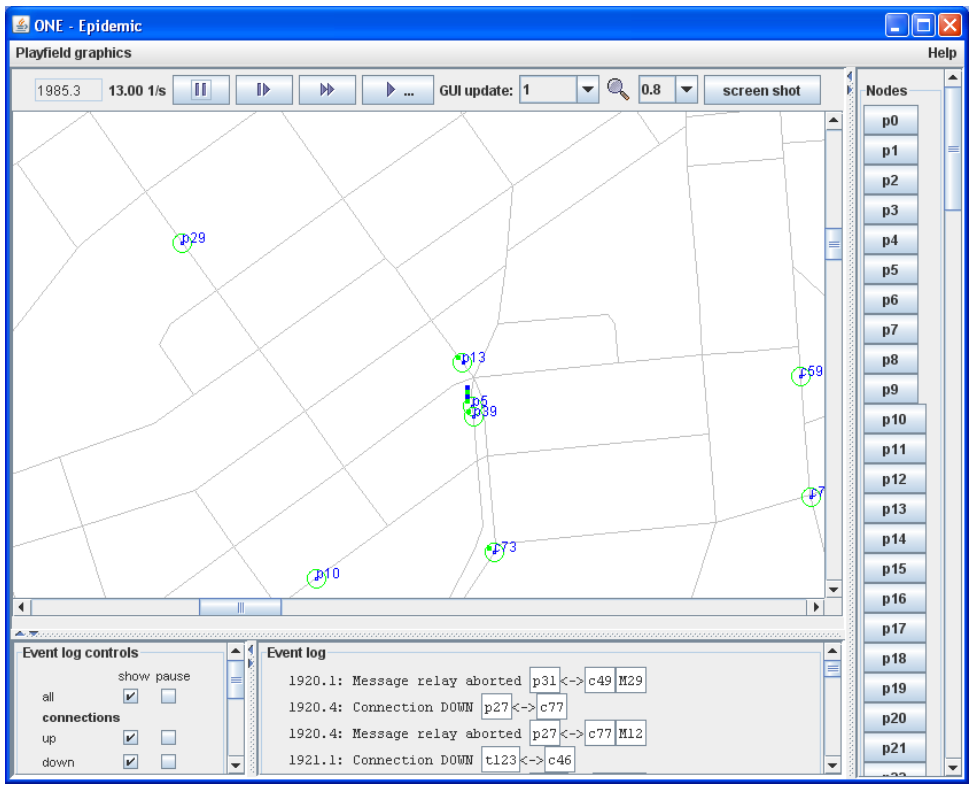
\includegraphics[width=1\textwidth]{figuras/cap_3/secao_1/interface_theONE.PNG}
    \caption{Interface do Simulador The ONE \cite{keranen2009one}.}
    \label{interface_theONE}
\end{figure}

\begin{figure}[htp!]
    \centering
    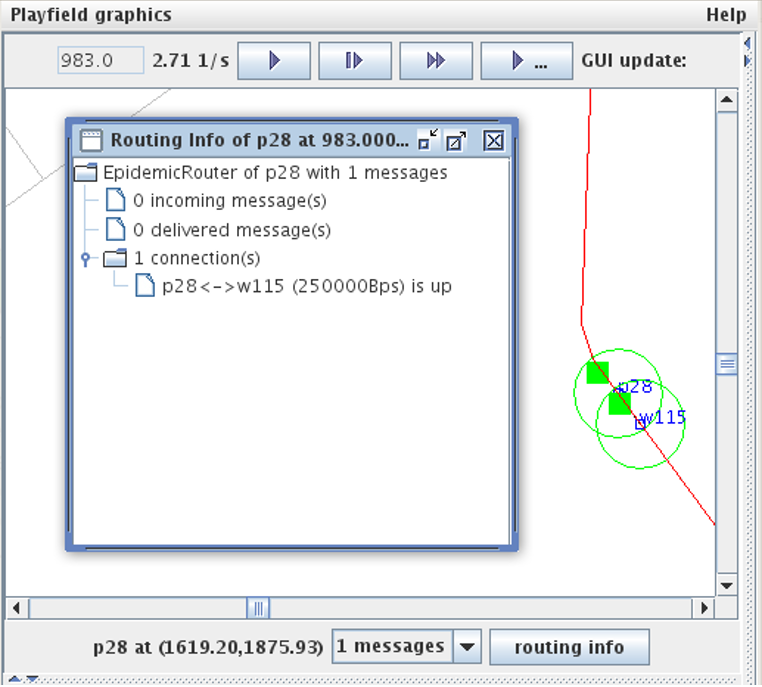
\includegraphics[width=0.6\textwidth]{figuras/cap_3/secao_1/node_theONE.PNG}
    \caption{Detalhes do nó \emph{p28} em uma simulação \cite{keranen2009one}.}
    \label{node_theONE}
\end{figure}

\newpage
\subsection{Arquivo de Configurações}
\label{subsec:arquivo_configuracao}
O arquivo de configurações do simulador consiste, basicamente, em um conjunto de linhas com definições de valores para os parâmetros de simulação. É a partir dele que o cenário de simulação é definido, incluindo, por exemplo, configurações dos grupos de nós, protocolos utilizados e modelos de movimento utilizados.

A Figura \ref{exemplo_config} apresenta um exemplo de trecho do arquivo de configurações do simulador The ONE. Nele é possível visualizar a definição de um cenário com o nome "exemplo". Por sua vez, este cenário apresenta um período de 86400 segundos, ou um dia, e possui apenas um único grupo de dispositivos. O grupo, que contém 10 nós,  utiliza uma interface \emph{Bluetooth} com alcance máximo de 10 metros e velocidade de transmissão de 25 KBytes/s. O protocolo escolhido foi o Epidemic Routing e os nós utilizam o modelo de movimentação \emph{ShortestPathMapBasedMovement} que, resumidamente, faz com que os nós sempre se movimentem pelos caminhos disponíveis no mapa escolhendo um ponto aleatório e seguindo a rota mais curta para este destino, a partir de sua localização atual. Além disso, existem configurações do módulo de energia, onde é definido que todos os nós do grupo possuem baterias com capacidade de 4800mW, consomem 0.92mW a cada busca por dispositivos e 0.08mW a cada segundo enviando ou recebendo mensagens.

\begin{figure}[htp!]
\centering
\lstinputlisting{codigos/exemplo.txt}
\caption{Exemplo de trecho do arquivo de configurações do simulador The ONE.}
\label{exemplo_config}
\end{figure}


\section{Java}\label{sec:java}

Java é uma plataforma e linguagem de programação de alto nível, baseada principalmente no paradigma orientado a objetos (OO), independente de plataforma e atrelada a um ambiente de execução integrado. Sua sintaxe é derivada de linguagens como C e C++, porém com abstrações e simplificações em relação ao modelo OO encontrado nesta última.  \cite{deitel2010java}

Aplicações Java são traduzidas para o bytecode (chamados de arquivos de classe ou class files) que são executados pela JVM (do inglês "Java Virtual Machine", ou "Máquina Virtual Java", em português), tendo um importante papel na plataforma, pois permite a portabilidade oferecida pela plataforma \cite{deitel2010java}. 

O conceito "write once, run anywhere" (ou "escreva uma vez, rode em qualquer lugar", em português) torna as aplicações extremamente portáveis, pois permite a criação de executáveis que podem ser executados em qualquer plataforma sem a necessidade de recompilação para cada uma delas \cite{deitel2010java}.

Abstrações relacionadas a gerencia de memória são implementadas pela JVM por meio do mecanismo de coleta de lixo (garbage-collector), proporcionando aos programadores maior facilidade na escrita de seus programas.

A figura \ref{ola_mundo_java} apresenta um simples código que escreve a célebre frase "Hello, world!" \newline no dispositivo de saída padrão de um computador.

\begin{figure}[htp!]
\centering
\lstinputlisting[language=Java]{codigos/ola_mundo.java}
\caption{Código Java que escreve a frase "Hello, world!" no dispositivo de saída padrão.}
\label{ola_mundo_java}
\end{figure}

Como já apresentado na seção \ref{sec:theONE}, o simulador the ONE foi implementado utilizando a plataforma Java. O desenvolvimento da técnica envolve a implementação de um módulo para o simulador utilizando essa linguagem, surgindo então a necessidade do estudo da mesma.

\section{Gnuplot}\label{sec:gnuplot}

Gnuplot é uma ferramenta gratuita capaz gerar gráficos a partir de funções matemáticas de duas ou três dimensões, e conjuntos de dados \cite{gnuplot5Doc}.

A geração de gráficos pode ocorrer diretamente na tela do computador ou ser direcionada para arquivos de diversos formatos, tais como JPEG, PNG, EPS e SVG. A criação automatizada de códigos LaTeX\footnote{Conjunto de macros para a confecção de textos Tex amplamente utilizada no meio acadêmico, principalmente por matemáticos, físicos e cientistas da computação.} é suportada, permitindo a inclusão simplificada diretamente nos documentos escritos nessa linguagem \cite{gnuplot5Doc}. 

Como visto em \cite{gnuplot5Doc}, o programa pode ser usado tanto interativamente, por meio de linhas de comando, quanto através de scripts em lote (batch mode). As figuras \ref{gnu_sincos} e \ref{gnu_sincos_code} apresentam um exemplo de gráfico gerado pela ferramenta e o seu código, respectivamente.

\begin{figure}[htp!]
\centering
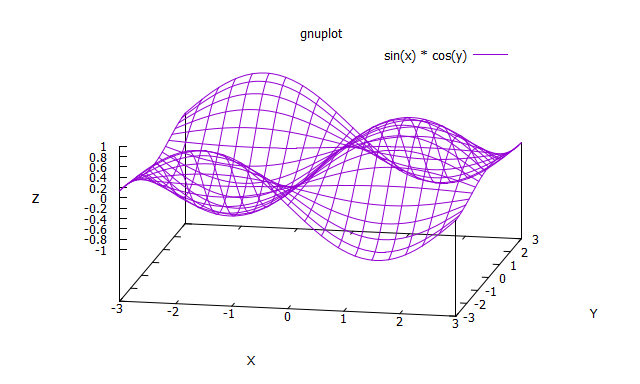
\includegraphics[width=1\textwidth]{figuras/cap_3/secao_3/gnuplot_sincos.png}
\caption{Gráfico gerado utilizando o gnuplot para a função $sin(x) . cos(y)$}
\label{gnu_sincos}
\end{figure}

\begin{figure}[htp!]
\centering
\lstinputlisting[language=gnuplot]{codigos/gnuplot.gnu}
\caption{Script utilizado para a geração do gráfico da figura \ref{gnu_sincos}}
\label{gnu_sincos_code}
\end{figure}

Dentro do contexto do trabalho, a utilização da ferramenta auxilia na geração de gráficos contendo os resultados dos testes, feitos por meio do simulador the ONE, e da análise dos resultados apresentados por meio de gráficos.

\section{Conclusão do Capítulo}\label{sec:conclusao_cap_3}

A primeira seção deste capítulo apresentou um breve resumo sobre o simulador the ONE, incluindo explanações sobre os protocolos implementados, arquitetura simplificada e funcionamento básico. Tal simulador é muito importante para o desenvolvimento da técnica objetivada, visto as facilidades oferecidas e o seu desempenho.

A linguagem Java, apresentada de forma sucinta na seção \ref{sec:java}, é de grande valia para a implementação da técnica, visto as abstrações oferecidas e a linguagem utilizada para o desenvolvimento do simulador.

A análise dos resultados da técnica é facilitada por meio dos relatórios gerados pelo simulador The ONE e da ferramenta gnuplot, apresentados nas seções \ref{sec:theONE} e \ref{sec:gnuplot}, respectivamente.

As ferramentas utilizadas são de grande importância para o projeto, contribuindo de forma significativa na construção da base necessária para o desenvolvimento e análise da técnica. Além disso, o estudo das ferramentas proporciona melhor entendimento e interação com assuntos relacionados às áreas de \emph{Simulação de Ambientes} e \emph{Probabilidade e Estatística}, permitindo adquirir conhecimentos não vistos durante o curso de Ciência da Computação.



%capítulo 4 - Descrição do Projeto
\chapter{DESCRIÇÃO DA TÉCNICA} \label{cap:tecnica}

Neste capítulo objetiva-se a descrição da técnica desenvolvida neste trabalho.

Inicialmente é apresentado o funcionamento da técnica quanto a forma como o mapeamento dinâmico é realizado e, posteriormente, como o intervalo de busca é calculado a partir do mapeamento. Em seguida a implementação da técnica é descrita juntamente com o diagrama de módulos atualizado do simulador e os parâmetros que podem ser ajustados dentro do ambiente simulado. Por fim, o capítulo é finalizado com uma conclusão a cerca dos assuntos debatidos.

\section{Funcionamento}

Como apresentado na subseção \ref{sec:definicoes}, as DTNs dependem das oportunidades de contato para a retransmissão de mensagens. Por sua vez, os contatos são influenciados diretamente pelo intervalo de busca por dispositivos próximos, visto que durante um período de espera um nó pode acabar não contatando outros que estava próximos. A partir daí, o gerenciamento do intervalo de busca de acordo com a probabilidade de contato numa determinada localização permite o ajusto dinâmico do intervalo fixo de espera de 32 segundos proposto por \cite{denis_artigo}.

O comportamento praticamente estocástico dos dispositivos, como os das moléculas de sacarose dissolvendo-se em água, torna a previsibilidade da localização dos contatos dificultosa em diversos cenários, como o das Redes Móveis Ad Hoc e o ZebraNet. Todavia, a concentração pode ser calculada por meio de um mapeamento dinâmico utilizando módulos de GPS dos dispositivos.

\subsection{O Mapeamento Dinâmico}

Inicialmente, uma divisão do mapa em regiões de igual tamanho é realizada. A partir daí, ao estabelecerem contato, os dispositivos envolvidos registram este em uma \emph{Tabela de Mapeamento de Regiões} (TMR). É por meio dessa tabela que cada nó tem uma visão global do mapa, pois sempre armazenam as quantidades de contatos registrados em cada uma das regiões pelas quais cada nó passou. Ao registrar um contato, é feita uma consulta GPS para determinar com precisão em que região o nó se encontra e contabilizar esse evento.

Após o registro do contato na tabela, os nós trocam suas TMRs para dinamizar o mapeamento e permitir que tenham acesso a dados de regiões pelas quais eles ainda não passaram. É passível de afirmação que o compartilhamento das TMRs implementa a prosa descrita na subseção \ref{subsec:gradientes_desafios}, onde dois nós, educadamente, compartilham um com o outro as informações que possuem acerca das regiões por onde passaram.

É de grande importância o estudo quanto a forma de mesclagem das tabelas de mapeamento. Durante o desenvolvimento deste trabalho foram consideradas três formas para tal, sendo elas:

\begin{itemize}
    \item \textbf{Mesclagem por Soma:} Nesta modalidade de mesclagem, para cada registro do nó contatado, se o dispositivo que recebeu a tabela, já possui alguma informação do registro é realizada uma soma dos valores. Caso contrário, o valor é adicionado a um novo registro na tabela. Em suma esta estratégia parece interessante, mas, durante as simulações, foi percebido que o comportamento cíclico de alguns nós causa a geração de registros extremamente discrepantes com relação ao comportamento real da rede, além de, após longos períodos de simulação, ocorrerem problemas com \emph{overflow} de variáveis mesmo quando utilizando \emph{64bits} de tamanho;
    \item \textbf{Mesclagem Incremental:} Ao realizar a mesclagem das tabelas, para cada registro do nó contatado, se o dispositivo já possui algum registro daquela região, é feito um incremento de um no registro local. Caso contrário, o valor é copiado para um novo registro na tabela. Esta abordagem não se mostrou satisfatória durante as simulações pois não conseguiu representar de forma satisfatória o comportamento real do mapa de regiões, ocorrendo momentos em que os valores ficaram totalmente incoerentes com a realidade;
    \item \textbf{Mesclagem por Substituição do Maior:} Nesta forma de mesclagem, para cada registro do outro nó, caso já exista um registro na tabela local e este seja menor que o do outro nó, é realizada a substituição. Caso não exista registro local, o valor é copiado. Caso contrário, ou seja, o valor local é maior que o do outro dispositivo, nada é feito. Esta forma de mesclagem foi a que melhor conseguiu representar o mapa regiões real, apresentando proporções coerentes com o comportamento real da rede.
\end{itemize}

Neste trabalho é considerada a mesclagem por meio da substituição do maior elemento devido ao fato de ter apresentado, durante as simulações, melhor representação do comportamento real da rede num ambiente onde o mapa é construído de forma independente e dinâmica.

Dados dois nós \emph{A} e \emph{B} localizados próximos e com o nó \emph{A} realizando buscas, o comportamento do mapeamento dinâmico é descrito pela Figura \ref{mapeamento}. É importante ressaltar que, neste trabalho, não foi considerada a sobrecarga gerada pela troca das TMRs.

\begin{figure}[htp!]
\centering
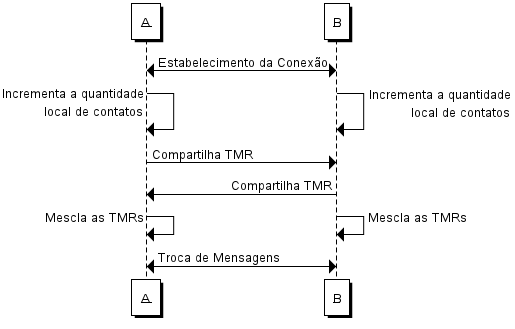
\includegraphics[width=0.75\textwidth]{figuras/cap_4/mapeamento.png}
\caption{Diagrama de Sequência do Mapeamento Dinâmico utilizando as TMRs}
\label{mapeamento}
\end{figure}

\subsection{Dinamização do Intervalo de Busca}
\label{sec:dinamizacao_intervalo_busca}
Tendo as Tabelas de Mapeamento de Regiões construídas dinamicamente, os dispositivos podem calcular livremente a probabilidade de contato em cada uma das regiões definidas previamente. Como pode ser visto em \cite{hazzan2013fundamentos}, a probabilidade de um evento $A$ ocorrer ($P(A)$), pode ser descrita por:

\begin{equation}
P(A)=\frac{n(A)}{n(\Omega)}
\end{equation}

Onde $n(A)$ é a quantidade de casos favoráveis a $A$ e $n(\Omega)$ é o número de resultados do experimento.

Tendo noção da probabilidade de contato $P(r)$ de um nó encontrar outro na região $r$, há duas decisões que um nó pode tomar: Aumentar ou diminuir o intervalo de buscas. Se um nó está em uma região com alta probabilidade de contato, este pode gastar mais a sua bateria visando aproveitar melhor as oportunidades daquela região. Caso a probabilidade seja muito pequena, o nó possui menor chance de tirar proveito de sua bateria, fazendo mais sentido economizá-la para um momento mais oportuno.

Observa-se então que, a concentração estimada em uma determinada região é, na verdade, a probabilidade de contato nessa localidade. A justificativa para isto baseia-se na grande importância dos contatos para as DTNs e na limitada visão que os dispositivos possuem quanto a quantidade de dispositivos próximos, visto hardware limitado que geralmente possuem. Além disso, regiões com altas taxas de contatos tendem a ser mais frequentadas por muitos dispositivos, influenciando diretamente na concentração efetiva da localidade.

Existe, entre a concentração, ou probabilidade de contado, e o intervalo de busca, um relacionamento de proporcionalidade inversa, ou seja, quanto maior a probabilidade, menor o intervalo de busca, e, quanto menor a probabilidade, maior o intervalo de busca. Sendo assim, é preciso descrever este relacionamento por meio de uma equação que o representa corretamente.

A proposta deste trabalho é que, dado um intervalo mínimo de busca $Im$, um intervalo máximo $IM$ pré-definidos e a probabilidade de contato na região em que o nó se encontra $P(r)$, pode-se descrever o intervalo de busca dito ideal $Ir$ como:

\begin{equation}
Ir=Im + (1-P(r))(IM-Im)
\label{eq_intervalo_ideal}
\end{equation}

O relacionamento de proporcionalidade inversa é descrito pelo termo $1-P(r)$, este pode ainda ser entendido como a probabilidade do contato não ocorrer \cite{hazzan2013fundamentos}. O termo $IM-Im$, quando multiplicado por $1-P(r)$ e posteriormente somado a $Im$, garante queo intervalo $Ir$ seja no máximo igual a $IM$  e no mínimo igual a $Im$.

O intervalo de busca ideal da região atual de um determinado nó da rede é calculado sempre quando este inicia um novo ciclo de busca que, por sua vez, nada mais é do que um período de procura por nós seguido de um intervalo de espera $Ir$ da região $r$ onde ele se encontra.

Quando a rede inicia sua operação, é notável que, durante certo período de tempo, os nós não possuem dados em suas TMRs ou estes ainda não são fieis ao comportamento estimado da rede. Para contornar este problema, foi proposto que a técnica passasse por um período de aquecimento, ou \emph{warmup time}, que é um período pré-definido onde os nós não fazem uso de suas TMRs e definem seus intervalos de busca como sendo o intervalo ideal de 32 segundos proposto por \cite{denis_artigo}.

Ainda existe o caso onde um determinado nó pode não ter dados sobre os contatos registrados na região onde ele se encontra. Para este caso, foi considerado o intervalo de busca de 32 segundos.

O diagrama da Figura \ref{diagrama} descreve de forma sucinta o funcionamento da técnica quanto a dinamização do intervalo entre as buscas por dispositivos.

\begin{figure}[htp!]
\centering
\includegraphics[width=0.75\textwidth]{figuras/cap_4/diagrama.png}
\caption{Diagrama de fluxo da dinamização do intervalo de busca}
\label{diagrama}
\end{figure}

\section{Descrição da Implementação}

A implementação da técnica dentro do simulador The ONE passou por duas etapas principais e importantes de serem descritas neste trabalho: a preparação do simulador e o desenvolvimento efetivo da técnica.

\subsection{Preparação do Simulador The ONE}

Antes do desenvolvimento efetivo da técnica, foi preciso preparar o simulador. É nesta etapa que o módulo de GPS foi implementado e sua respectiva incorporação com o módulo de energia foi feita.

O módulo de GPS nada mais é que uma classe \emph{GPSModule} integrada à classe \emph{DTNHost} que, por sua vez, é responsável por representar cada nó da rede simulada. 

O \emph{GPSModule} possui dois modos de operação. São eles:

\begin{itemize}
    \item \textbf{Com consumo:} É modo utilizado para contabilização de energia consumida pelo dispositivo de GPS integrado aos hosts. A cada consulta GPS o \emph{GPSModule} se encarrega de notificar ao módulo de energia \emph{EnergyModel} que este foi utilizado e consumiu a bateria.
    \item \textbf{Sem consumo:} É o modo utilizado para simulações quando não se deseja contabilizar o consumo do dispositivo de GPS.
\end{itemize}

Devido ao fato dos dispositivos GPS também serem responsáveis pelo consumo das baterias, o módulo desenvolvido também é integrado ao módulo de energia do simulador. A contabilização do consumo é feita a cada consulta GPS realizada pelo dispositivo a partir da chamada ao método \emph{reduceEnergy} explanado na subseção \ref{modulo_energia}.

A forma como o módulo foi implementado permite que o usuário defina padrões de consumo para cada um grupo de nós. Como exemplo, é possível criar dois grupos um para \emph{smartphones} e outro para carros e definir um consumo diferente de energia para cada um deles. Caso seja desejado, é possível ainda definir um consumo global, onde todos os nós respeitam um único padrão de consumo.

A utilização do módulo necessita da definição da quantidade de energia que é consumida pelo dispositivo GPS em cada consulta. Essa configuração se dá por meio da propriedade \emph{gpsScanEnergy} dentro do arquivo de configurações do simulador apresentado na subseção \ref{subsec:arquivo_configuracao}. Em caso da omissão dessa linha de configuração, o simulador entenderá que modo de operação é o \emph{sem consumo} e, consequentemente, não contabilizará o consumo de energia por parte dos dispositivos GPS.

A Figura \ref{gps_config} apresenta um exemplo de configuração onde todos os dispositivos são configurados para consumirem 154,6mW em cada consulta GPS.

\begin{figure}[htp!]
\centering
\lstinputlisting[language=Java]{codigos/gps_config.txt}
\caption{Exemplo de configuração do consumo do módulo de GPS.}
\label{gps_config}
\end{figure}

\subsection{Desenvolvimento da Técnica}

A técnica desenvolvida teve seu foco principal na modelagem da \emph{Tabela de Mapeamento de Regiões}, no modelo de ajuste de busca e na integração deles com o simulador.

A TMR foi implementada pela classe \emph{ConcentrationMap}, que, por sua vez, utiliza uma tabela de dispersão para armazenar as informações das regiões definidas por meio do tamanho base \emph{RegionLength}. Esta estratégia de armazenamento permite economia de memória, visto que apenas as regiões com dados conhecidos são armazenadas pelo dispositivo.

O modelo de ajuste de busca, definido pelo \emph{ScanAdjustmentModel}, é responsável pela dinamização do intervalo de busca por dispositivos. É nele que se encontra o método \emph{getBestScanTime}, responsável por realizar o cálculo da equação \ref{eq_intervalo_ideal}, apresentada na subseção \ref{sec:dinamizacao_intervalo_busca}, e retornar o intervalo apropriado para a região em que o nó se encontra. Além dos intervalos mínimos e máximos de busca, representados pelos parâmetros \emph{MinScanInterval} e \emph{MaxScanInterval}, respectivamente, o método também recebe o parâmetro \emph{DefaultScanInterval}, que, por sua vez, representa o intervalo de busca padrão a ser utilizado quando em \emph{warmup time} ou quando o dispositivo não possui dados sobre a região onde se encontra.

É importante ressaltar que, o intervalo padrão pode ser ajustado livremente pelo usuário, mas, neste trabalho, considerou-se apenas o intervalo ideal proposto por \cite{denis_artigo}, ou seja, 32 segundos, como visto na Figura \ref{diagrama}.

Tendo a TMR e o modelo de ajuste de busca implementados, foi necessário integrá-los ao simulador. Para isso a interface de rede dos nós, representada pela classe \emph{NetworkInterface}, precisou ser alterada. Em suma, apenas o método \emph{isScanning} foi modificado para utilizar o intervalo de busca apropriado (retornado pelo método \emph{getBestScanTime}) quando detecta que um novo ciclo de busca foi iniciado.

Dentro da arquitetura do simulador, o resultado das alterações feitas é apresentado no diagrama da Figura \ref{theOne_modificado}. A técnica em si, foi implementada dentro do módulo \emph{Conectivity and Data} e é representada em laranja como \emph{TMR and GPS module}.

A Figura \ref{tecnica_config} exibe um exemplo de configuração para todos os dispositivos dos parâmetros \emph{DefaultScanInterval}, \emph{MinScanInterval}, \emph{MaxScanInterval}, \emph{RegionLength} e \emph{AdjustmentWarmup}.

A Tabela \ref{parametros_ajustaveis} apresenta individualmente os parâmetros da técnica que podem ser ajustados para a descrição do cenário de simulação dentro do arquivo de configurações do simulador apresentado na Subseção \ref{subsec:arquivo_configuracao}.
\begin{figure}[htp!]
\centering
\includegraphics[width=1\textwidth]{figuras/cap_4/TheONEArchtecture_modificada.png}
\caption{Diagrama de fluxo da dinamização do intervalo de busca}
\label{theOne_modificado}
\end{figure}

\begin{figure}[htp!]
\centering
\lstinputlisting[language=Java]{codigos/tecnica_config.txt}
\caption{Configuração dos parâmetros de funcionamento da técnica.}
\label{tecnica_config}
\end{figure}


\begin{table}[H]
\centering
\caption{Parâmetros ajustáveis da técnica.}
\begin{tabular}{|l|l|l|}
\hline
\textbf{Parâmetro}        & \textbf{Tipo}   & \textbf{Ação}                                                      \\ \hline
GpsScanEnergy    & double & \begin{tabular}[x]{@{}l@{}}Define a quantidade de energia gasta a cada busca\\de GPS.\end{tabular} \\ \hline
MinScanInterval  & double & Define o intervalo mínimo de busca.                       \\ \hline
MaxScanInterval  & double & Define o intervalo máximo de busca.                       \\ \hline
DefaultScanInterval  & double & Define o intervalo padrão de busca.                       \\ \hline
AdjustmentWarmup & int    & Define o tempo de aquecimento da técnica.                 \\ \hline
RegionLength     & double & Define o tamanho das regiões.                             \\ \hline
\end{tabular}
\label{parametros_ajustaveis}
\end{table}


\section{Conclusão do Capítulo}

Neste capítulo foi apresentado o funcionamento da técnica desenvolvida e como esta foi implementada dentro do simulador The ONE. Além disso foram apresentados os parâmetros que a técnica permite que sejam alterados.

A partir do momento em que a técnica foi finalizada, o próximo passo é demonstrar seu comportamento nos cenários de teste escolhidos, permitindo avaliar os dados coletados e, finalmente, determinar se a sua aplicabilidade num ambiente real é viável ou não. Tal demonstração e avaliação são apresentadas no capítulo \ref{cap:testes}.

%capítulo 5 - Testes
\chapter{TESTES DE DESEMPENHO DA TÉCNICA} \label{cap:testes}

É objetivo deste capítulo abordar detalhes relacionados aos testes de desempenho da técnica desenvolvida.

Inicialmente é realizado o detalhamento dos cenários de testes, incluindo detalhes do ambiente geográfico definido e dos dispositivos que compõem a rede simulada. Após isso, são apresentados, por meio de gráficos, e discutidos os resultados dos testes realizados.

É importante ressaltar que, neste capítulo, o termo GPS é utilizado como sinônimo para qualquer tipo de aparelho que possa, por meio de satélites, determinar a sua posição no globo terrestre.

\section{Cenário de Testes}
\label{sec:cenario}

Dentro do âmbito das DTNs, é possível dissertar acerca de uma imensa quantidade de cenários possíveis para teste. Tendo em isso em vista, decidiu-se, neste trabalho, basear-se no cenário de testes definido em \cite{denis_artigo}. Além disso, foram considerados os dois estados da técnica desenvolvida: Desligada e Ligada contabilizando o consumo de GPS. Contabilizar o consumo GPS possibilita uma análise aprofundada do consumo adicional gerado pela técnica devido ao uso desses dispositivos.

O mapa da Figura \ref{mapa_tecnica} foi utilizado como base para os testes realizados e possui uma dimensão de 4500 por 3500 metros. O mesmo é baseado na cidade Helsínquia, a capital da Finlândia. A Figura \ref{mapa_helsinquia} apresenta uma sobreposição do mapa do ambiente simulado com o da cidade escolhida, permitindo perceber grande similaridade entre eles. Este mesmo mapa foi utilizado por \cite{denis_artigo}.

\begin{figure}[htp!]
\centering
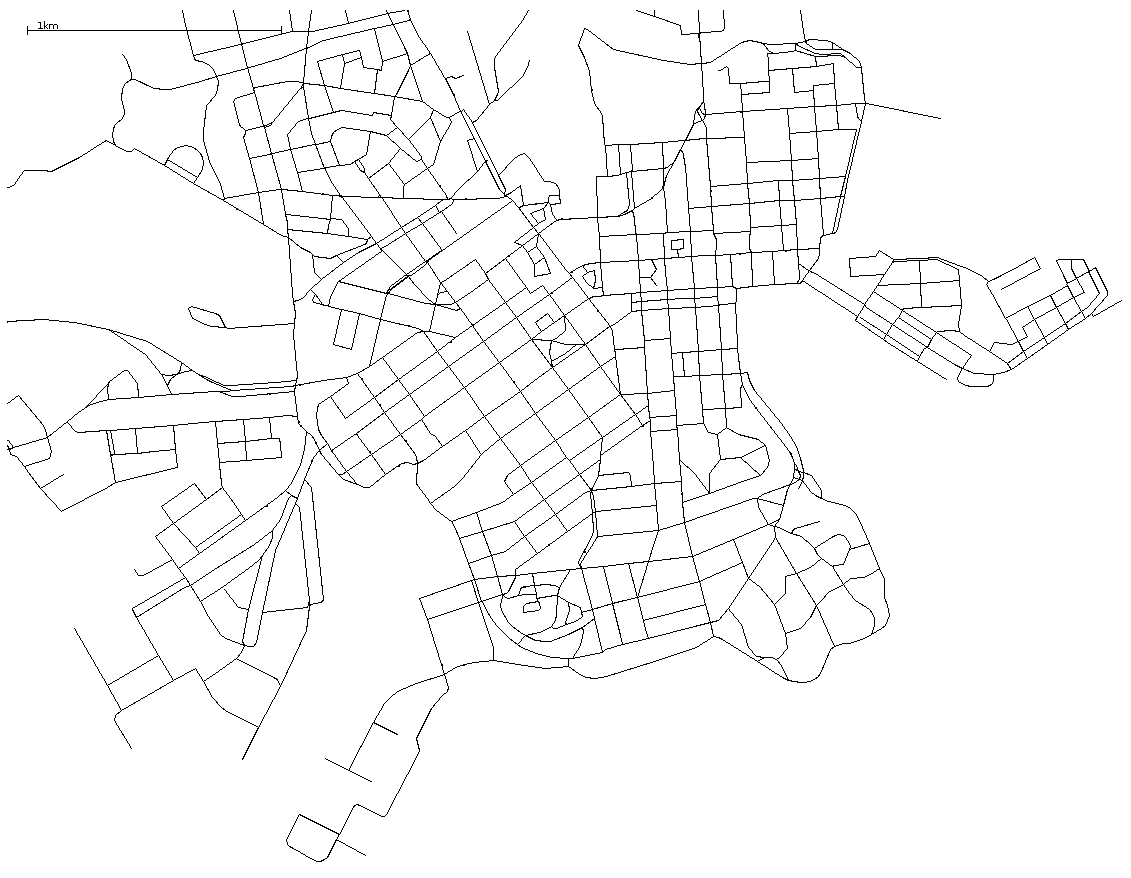
\includegraphics[width=0.9\textwidth]{figuras/cap_5/mapa.png}
\caption{Mapa utilizado nos cenários de teste \cite{keranen2009one}.}
\label{mapa_tecnica}
\end{figure}

\begin{figure}[htp!]
\centering
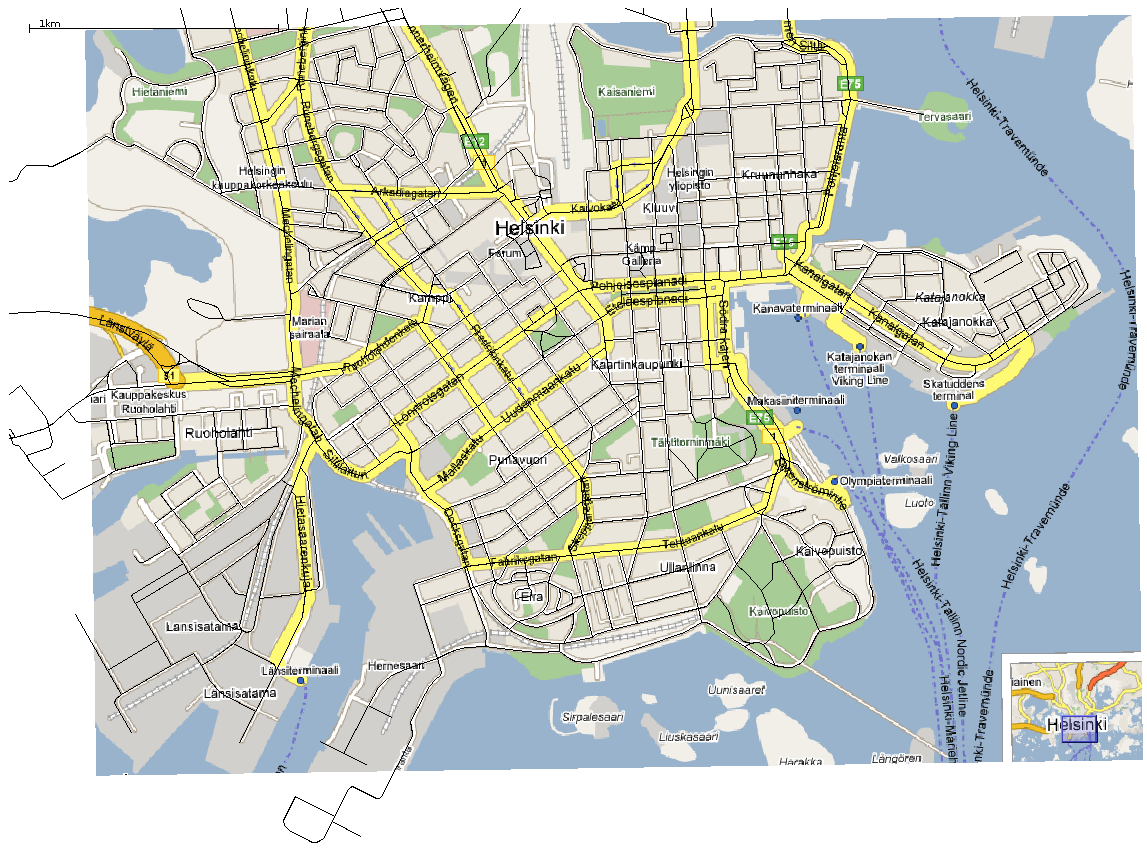
\includegraphics[width=0.9\textwidth]{figuras/cap_5/mapa_helsinquia.png}
\caption{Mapa da cidade Helsínquia \cite{keranen2009one}.}
\label{mapa_helsinquia}
\end{figure}

Foram definidas regiões quadradas com 500 metros de lado, totalizando assim um conjunto de 63 regiões. Este valor foi escolhido devido a multiplicidade com o tamanho do mapa base e por não gerar uma quantidade exorbitante de regiões a serem mapeadas. Quando objetivada uma mais análise aprofundada, este parâmetro é passível de ser verificado quanto a procura de um tamanho ideal que se adeque a limitações de memória que os dispositivos utilizados possuem e características relacionadas ao comportamento da DTN onde a técnica será utilizada.

A DTN proposta é constituída por 51 nós divididos em seis grupos. Dois deles, \emph{p} e \emph{w}, com 15 elementos cada, representam grupos de pedestres. Existe um grupo \emph{c} de 15 nós representando carros e, outros três grupos \emph{th}, \emph{tr} e \emph{tu}, com dois elementos cada, representando os bondes da cidade de Helsínquia. 

Os grupos pedestres se locomovem respeitando o modelo de movimento Shortest Path Map-Based Movement, onde os nós sempre se movimentam pelos caminhos disponíveis no mapa escolhendo pontos aleatórios e seguindo até eles pela rota mais curta partindo da sua posição atual. A velocidade com que as pessoas se movimentam pode variar entre 1,8 a 5,5 Km/h. Os carros no cenário desenvolvido utilizam o mesmo modelo de movimento dos pedestres, todavia são forçados se locomover apenas pelas ruas e desenvolvem velocidades entre 10 e 50 Km/h.

Os grupos de bondes utilizam o modelo de movimento Routed Map-Based Moviment. Neste modelo cada grupo de nós sempre se locomove por uma rota distinta dos demais. Por se tratar de bondes, os mesmos realizam paradas em locais pré-determinados por períodos de dez a trinta segundos. A velocidade desses nós varia de 25 e 36 km/h. 

A Tabela \ref{grupos_nos} apresenta de forma sucinta os dados dos grupos de nós definidos para o cenário de simulação.

Devido a uma limitação do simulador The ONE, não é possível que pessoas entrem e saiam dos carros e bondes. Para contornar isso, assumiu-se que os condutores de cada um dos veículos portam o mesmo tipo dispositivo utilizado pelos pedestres. Por sua vez, os dispositivos utilizados por todos os indivíduos da rede constem em \emph{smartphones} com baterias de 4800mW e interfaces \emph{bluetooth} para a troca de mensagens. As interfaces \emph{bluetooth} possuem um alcance de 10 metros e velocidade de transmissão de 2Mb/s. Além disso, os aparelhos possuem uma capacidade de armazenamento de 5MB.

\begin{table}
\centering
\caption{Definição dos grupos de nós.}
\label{grupos_nos}
\begin{tabular}{|c|c|c|c|c|}
\hline
Nome          & Tipo      & Velocidade     & Quantidade & Modelo de Movimento               \\ \hline
p             & Pedestres & 1,8 a 5,5 Km/h & 15         & ShortestPath  Map-Based \\ \hline
c             & Carros    & 10 a 50 Km/h   & 15         & ShortestPath  Map-Based \\ \hline
w             & Pedestres & 1,8 a 5,5 Km/h & 15         & ShortestPath  Map-Based  \\ \hline
th            & Bonde     & 25 a 36 Km/h   & 2          & Routed Map-Based         \\ \hline
tr            & Bonde     & 25 a 36 Km/h   & 2          & Routed Map-Based         \\ \hline
tu            & Bonde     & 25 a 36 Km/h   & 2          & Routed Map-Based         \\ \hline
\end{tabular}
\end{table}

Os parâmetros de energia, essenciais neste trabalho, seguem também o mesmo modelo de consumo proposto por \cite{denis_artigo} e são apresentados na Tabela \ref{consumo_denis_artigo}. Os \emph{smartphones} iniciam com a bateria totalmente carregada e ela vai descarregando a medida em que fazem operações de busca, envio e recepção de mensagens. Adicionalmente, é considerado o consumo dos dispositivos GPS explanado na Subseção \ref{subsec:consumo_gps}, ou seja, 154,6mW a cada consulta realizada. 

\begin{table}
\centering
\caption{Parâmetros de energia utilizados.}
\label{consumo_denis_artigo}
\begin{tabular}{|c|c|}
\hline
Parâmetros                   & Definições    \\ \hline
Capacidade da bateria        & 4800mW        \\ \hline
Consumo da Busca             & 0.92mW/busca \\ \hline
Consumo enviando mensagem    & 0.08mW/s\\ \hline
Consumo recebendo mensagem   & 0.08mW/s\\ \hline
Consumo do dispositivo GPS   & 0.1546mW/consulta \\ \hline
\end{tabular}
\end{table}

Quanto aos protocolos de encaminhamento, foram considerados os protocolos \emph{Epidemic Routing}, \emph{Prophet} e \emph{Spray-and-Wait}, detalhados na Subseção \ref{subsec:encaminhamento_mensagens}. 

Além disso, é inerente, na análise de desempenho da técnica, levar em consideração a procura por um intervalo de busca ótimo. No entanto, optou-se neste trabalho por estudá-lo em apenas duas combinações próximas ao período de 32 segundos apresentado por \cite{denis_artigo}. A primeira, com 8, 32 e 56 segundos, com variação de 16 segundos para mais e para menos; a segunda, com 8, 32 e 32 segundos, com apenas uma variação de 16 segundos para menos. Os valores se referem à ordem dos intervalos de cada combinação, sendo o mínimo, padrão e máximo, respectivamente.

Os tempos de simulação consistem em períodos de 10 e 30 dias e são realizadas análises quanto a recarga periódica completa das baterias.

\section{Discussão dos Resultados Obtidos}

É objetivo desta seção apresentar e discutir os resultados obtidos a partir dos testes da técnica desenvolvida com o intuito de avaliar seu desempenho quanto a entrega de mensagens e seu consumo energético. Além disso, são discutidos os resultados obtidos quando a recarga das baterias é considerada com o intuito de analisar o comportamento a longo prazo.

Os resultados são apresentados na forma de gráficos, onde cada um deles são associados a uma das primeiras três letras do alfabeto, ou seja, as letras \emph{a}, \emph{b} e \emph{c}. A primeira delas é associada aos gráficos que apresentam o comportamento da rede quanto a probabilidade de entrega de mensagens; a segunda é combinada aos que exibem o comportamento quanto a quantidade de mensagens entregues aos destinatários; a última é relacionada a gráficos que apontam o comportamento médio da quantidade de energia armazenada nas baterias dos dispositivos. Cada um gráficos apresenta o comportamento da rede para cada um dos três protocolos testados e, simultaneamente, para os dois estados da técnica, ou seja, ligada (considerando o consumo dos dispositivos GPS) e desligada. 

\subsection{Desconsiderando Recarga Periódica}

Desconsiderar recargas periódicas permite analisar como a rede se comporta quanto ao consumo efetivo das baterias e entregas de mensagens em um curto período de tempo. Além disso, a visualização de pontos ideais de recarga é facilitada, permitindo testá-los e visualizar o comportamento da rede em longo prazo.

Nesta Subseção são apresentados e discutidos os resultados obtidos desconsiderando a recarga periódica das baterias para os dois períodos de busca propostos na Seção \ref{sec:cenario}, ou seja, 8, 32 e 56 segundos e 8, 32 e 32 segundos. referindo-se à ordem dos intervalos de cada combinação, sendo o mínimo, padrão e máximo, respectivamente.

\newpage
\subsubsection{Intervalo Busca de 8, 32 e 56 Segundos}
\label{8-32-56_semRecarga}

Quando se trata do intervalo de 8, 32 e 56 segundos, sendo o período de busca mínimo, padrão e máximo, respectivamente, a rede apresenta o comportamento apresentados nos gráficos da Figura \ref{10dias_8-32-56_semRecarga}.

É visto no gráfico \emph{c} que a técnica gera um maior consumo das baterias, o que se traduz na morte da rede por volta do final do sétimo dia de simulação. A falta de energia causa a interrupção na entrega de mensagens, como visto no gráfico \emph{b}, e, consequentemente a queda da probabilidade de entrega, apresentada no gráfico \emph{a}.

Pelos gráficos \emph{a} e \emph{b} é possível observar que, durante o tempo de atividade da rede a técnica não consegue se sobressair com relação a quantidade de mensagens entregues e, consequentemente, quanto a probabilidade de entrega. Isso, quando associado ao consumo adicional das baterias observado no gráfico \emph{c}, é entendido como um não aproveitamento da energia adicional consumida, pois não foi capaz de aumentar a quantidade de mensagens entregues.

A justificativa do consumo adicional das baterias é de simples argumentação. Ele se deve, primordialmente, ao consumo adicional gerado pelos dispositivos GPS, visto que, sem a técnica, estes dispositivos não são utilizados. Além disso, o consumo adicional gerado pela redução do intervalo de busca para até 8 segundos não é compensado pelo aumento até os 56 segundos.

Além disso, pode-se observar que os três protocolos apresentam uma linha de tendência semelhante. Todavia, é percebida uma ligeira vantagem do protocolo \emph{Prophet} em relação aos demais quanto a entrega de mensagens, gráfico \emph{b}, e a probabilidade de entrega, gráfico \emph{a}. Esse resultado permite observar a vantagem dos protocolos probabilísticos em relação aos não probabilísticos apresentada na Subseção \ref{subsec:encaminhamento_mensagens}.

Quando considerados os fatores apresentados, observa-se que a técnica não traz vantagens quando utilizada com os parâmetros definidos, visto que o consumo adicional das baterias não se traduziu no aumento da quantidade de mensagens entregues e, consequentemente, numa maior probabilidade de entrega de mensagens.

\begin{sidewaysfigure}
\centering
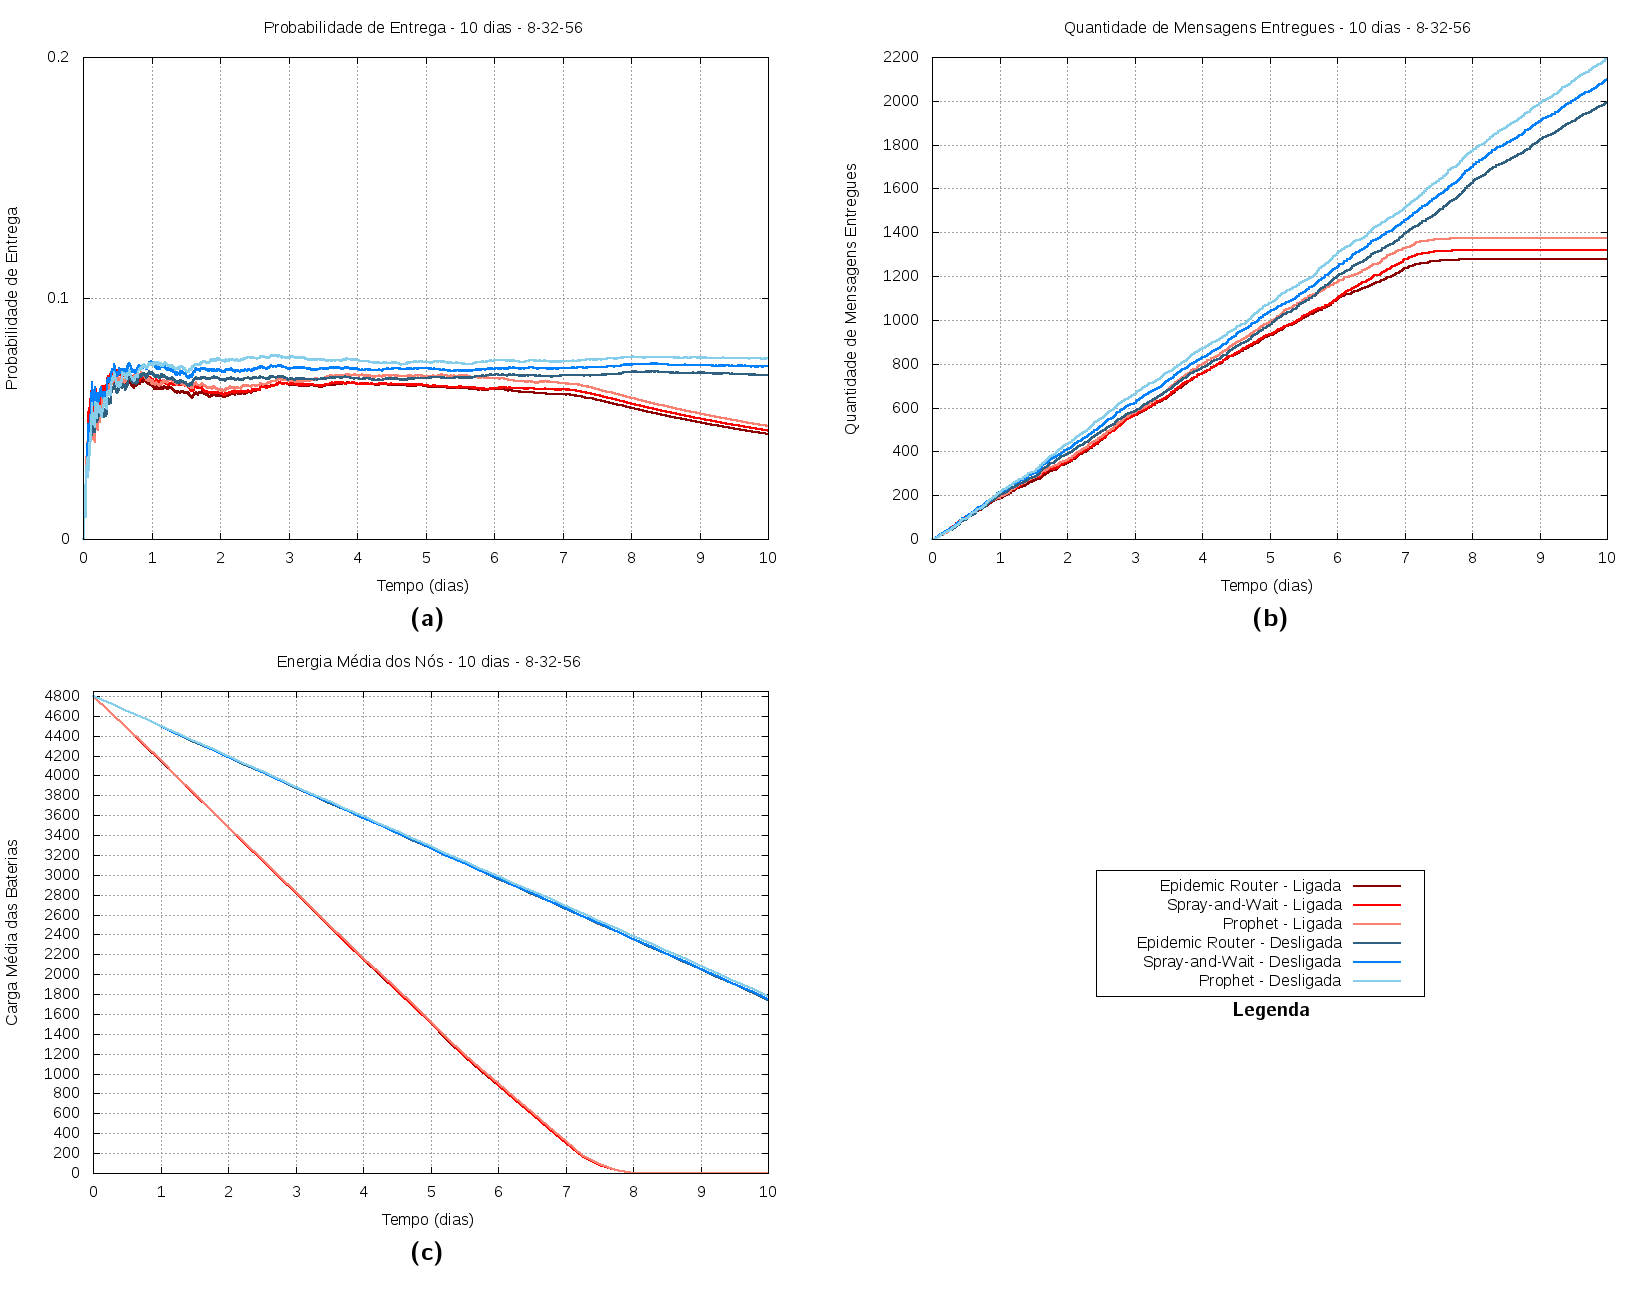
\includegraphics[width=0.8\textwidth]{figuras/cap_5/graficos/8_32_56/MessageDeliveryReport_10_8-32-56_noRecharge.png}
\caption{Resultados de simulações de 10 dias sem recarga periódica e período de busca de 8, 32 e 56 segundos.}
\label{10dias_8-32-56_semRecarga}
\end{sidewaysfigure}

\newpage
\subsubsection{Intervalo de Busca de 8, 32 e 32 Segundos}
\label{8-32-32_semRecarga}

Quando se trata do intervalo de 8, 32 e 32 segundos, sendo o período de busca mínimo, padrão e máximo, respectivamente, a rede apresenta o comportamento apresentados nos gráficos da Figura \ref{10dias_8-32-32_semRecarga}.

A redução do período de busca, que agora pode variar apenas dentro do intervalo de 8 a 32 segundos, acarretou num aumento significativo do consumo das baterias dos dispositivos, como visto no gráfico \emph{c}, reduzindo pela metade o tempo de vida da rede. Todavia, como visto nos gráficos \emph{a} e \emph{b}, a probabilidade de entrega e, consequentemente, a quantidade de mensagens entregues aumentaram significativamente durante o período de atividade da rede.

Os resultados obtidos quanto a quantidade de mensagens entregues durante o período de atividade da rede podem ser facilmente explicados. Eles são decorrentes da redução do período onde o intervalo de busca se situa, ou seja, de 8 a até 56 segundos para 8 a até 32 segundos, o que faz com que os dispositivos passem menos tempo aguardando por novos ciclos de busca, traduzindo-se numa maior quantidade de buscas por dispositivos. 

Aumentar a quantidade de buscas por outros dispositivos resulta num aumento da quantidade tempo que os dispositivos passam buscando por outros. Consequentemente, contatos que antes seriam perdidos devido aos dispositivos estarem aguardando por outro ciclo de busca ocorrem com menor frequência. Finalmente, há uma maior quantidade de oportunidades de contato, o que resulta num aumento da quantidade de mensagens entregues e na probabilidade de entrega de mensagens durante o período de atividade da rede.

O ajuste dinâmico, provido pela técnica a partir do uso das tabelas de mapeamento, garante que os intervalos entre as buscas fiquem menores em regiões com alta probabilidade de contato, aumentando ainda mais a quantidade deles devido ao melhor aproveitamento das baterias em situações onde aumentar o consumo é uma decisão inteligente.

Em decorrência da maior quantidade de mensagens entregues, durante o período de atividade da rede, a probabilidade de entrega se manteve acima da rede que não utiliza a técnica. Ao interromper suas atividades por falta de energia, a rede não entrega mais mensagens e, como consequência, a probabilidade de entrega cai gradativamente até que esta fique menor que a da rede que não utiliza a técnica desenvolvida.

A morte prematura da rede torna ineficiente a utilização da técnica quando não é considerada a recarga das baterias dentro do cenário analisado. Todavia, a vantagem da técnica durante o período de atividade da rede pode ser melhor explorada quando é considerada a recarga.

\begin{sidewaysfigure}
\centering
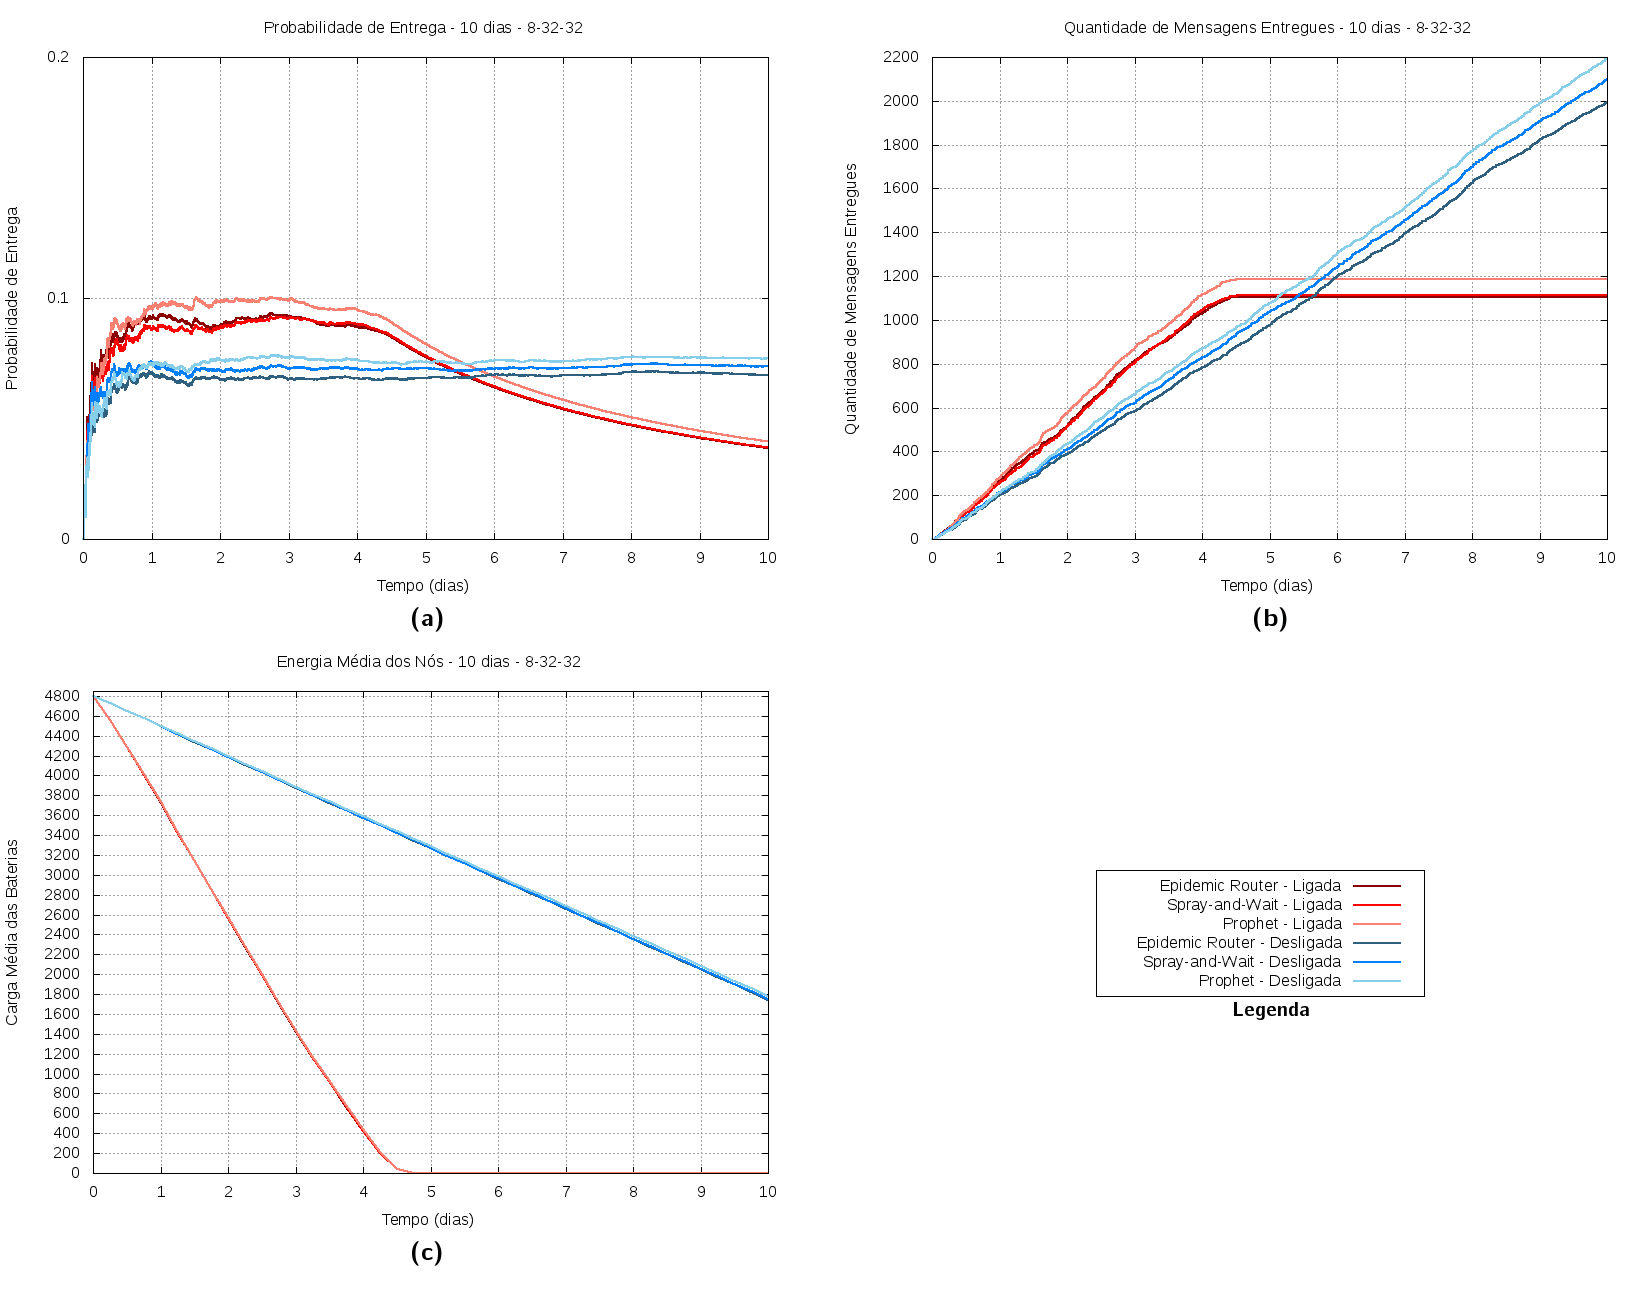
\includegraphics[width=0.8\textwidth]{figuras/cap_5/graficos/8_32_32/MessageDeliveryReport_10_8-32-32_noRecharge.png}
\caption{Resultados de simulações de 10 dias sem recarga periódica e período de busca de 8, 32 e 32 segundos.}
\label{10dias_8-32-32_semRecarga}
\end{sidewaysfigure}

\subsubsection{Discussões Sobre o Cenário sem Recarga das Baterias}

Dentro dos intervalos testados, o que apresentou pior desempenho foi o de 8, 32 e 56 segundos. Este resultado é decorrente da ineficiência quanto ao consumo adicional gerado pela técnica devido ao uso de dispositivos GPS e a quantidade inferior de mensagens entregues ao ser comparada com uma DTN que não a utiliza. Quando a linha de tendência dos gráficos da Figura \ref{10dias_8-32-56_semRecarga} é analisada, é possível concluir que durante o tempo de vida da rede, mesmo quando realizadas recargas, não ocorrerão melhorias quanto a quantidade de mensagens entregues. Essa situação é verificada logo a seguir.

O intervalo de 8, 32 e 32 segundos apresentou um desempenho consideravelmente melhor quanto a probabilidade de entrega e quantidade de mensagens entregues durante o tempo de vida da rede. Esse resultado é proveniente do consumo inteligente das baterias atrelado a redução do período que o intervalo de busca se situa. Quando analisa-se linha de tendência da quantidade de mensagens entregues, percebe-se que, durante o tempo de atividade da rede, a técnica apresenta vantagens e estas podem ser aproveitadas quando a recarga das baterias é considerada. Esta situação será verificada na Subseção \ref{subsec:testes_com_recarga}.

Analisando a fundo o consumo adicional de energia gerado pela técnica, é percebido que quanto menor for o intervalo de busca ideal de uma região, maior é o consumo de energia. Isso se deve ao fato de que uma consulta GPS precisa ser realizada quando os dispositivos precisam calcular o novo período de espera, como apresentado na Subseção \ref{sec:dinamizacao_intervalo_busca}. Além disso, quanto menor esse período, maior a quantidade de buscas e, consequentemente, maior ainda a energia consumida por esses componentes.

Finalmente, quando considerado um cenário onde não existe a possibilidade de recarga das baterias, a técnica apresenta desvantagem, visto que os testes indicaram a morte prematura da rede quando ela é utilizada.

\subsection{Considerando Recarga Periódica}
\label{subsec:testes_com_recarga}

Dentro do âmbito das DTNs, a recarga periódica de baterias é possível em diversos cenários, exemplificando-se com o uso de placas solares em situações como as aplicações espaciais e o projeto ZebraNet \cite{zhang2004hardware}. Além disso, considerar a recargadas baterias permite analisar o comportamento da técnica a longo prazo.

Nesta Subseção são apresentados e discutidos os resultados obtidos considerando a recarga periódica das baterias para os dois períodos de busca propostos na Subseção \ref{sec:cenario}, ou seja, 8, 32 e 56 segundos e 8, 32 e 32 segundos, sendo os intervalos mínimo, padrão e máximo, respectivamente.

\subsubsection{Intervalo de Busca de 8, 32 e 56 Segundos}
\label{8-32-56_comRecarga}

A partir da análise do gráfico \emph{c} da Figura \ref{10dias_8-32-56_semRecarga}, conclui-se que todos os dispositivos da rede têm suas baterias esgotadas ao final do sétimo dia. Partindo disso pode-se definir um intervalo máximo de recarga no exato ponto onde a rede encerra a sua atividade para analisar o seu comportamento a longo prazo.

Num cenário de 10 dias de simulação e com um período de recarga de sete dias, foi observado o comportamento dos gráficos da Figura \ref{10dias_8-32-56_comRecarga}. No gráfico \emph{a} pode ser visto que a probabilidade de entrega da técnica encontra-se abaixo em relação a uma rede que não a utiliza. A probabilidade de entrega é refletida na quantidade de mensagens entregues que, por sua vez, também apresenta desvantagem, como visto no gráfico \emph{b} da mesma Figura. Pode ser observado que os resultados estão de acordo com a linha de tendência observada nos resultados apresentados na Figura \ref{10dias_8-32-56_semRecarga} durante o tempo de atividade da rede simulada.

A longo prazo, num período de 30 dias, a rede apresenta o comportamento visto na Figura \ref{30dias_8-32-56_comRecarga}, onde pode ser observada a mesma linha de tendência da Figura \ref{10dias_8-32-56_comRecarga}, tanto para a probabilidade de entrega quanto para a quantidade de mensagens entregues. A probabilidade de entrega utilizando a técnica, apresentada no gráfico \emph{a}, se mantém estável porém abaixo da rede que não a utiliza. O gráfico \emph{b} reflete a situação do gráfico \emph{a}, onde a quantidade de mensagens entregues também se mantém abaixo de uma rede sem a técnica. Com a técnica 5706 mensagens foram entregues contra 6170 mensagens sem ela, ou seja, uma diferença de 464 mensagens. Todos os valores referem-se as quantidades médias dos dados observados.

\begin{sidewaysfigure}
\centering
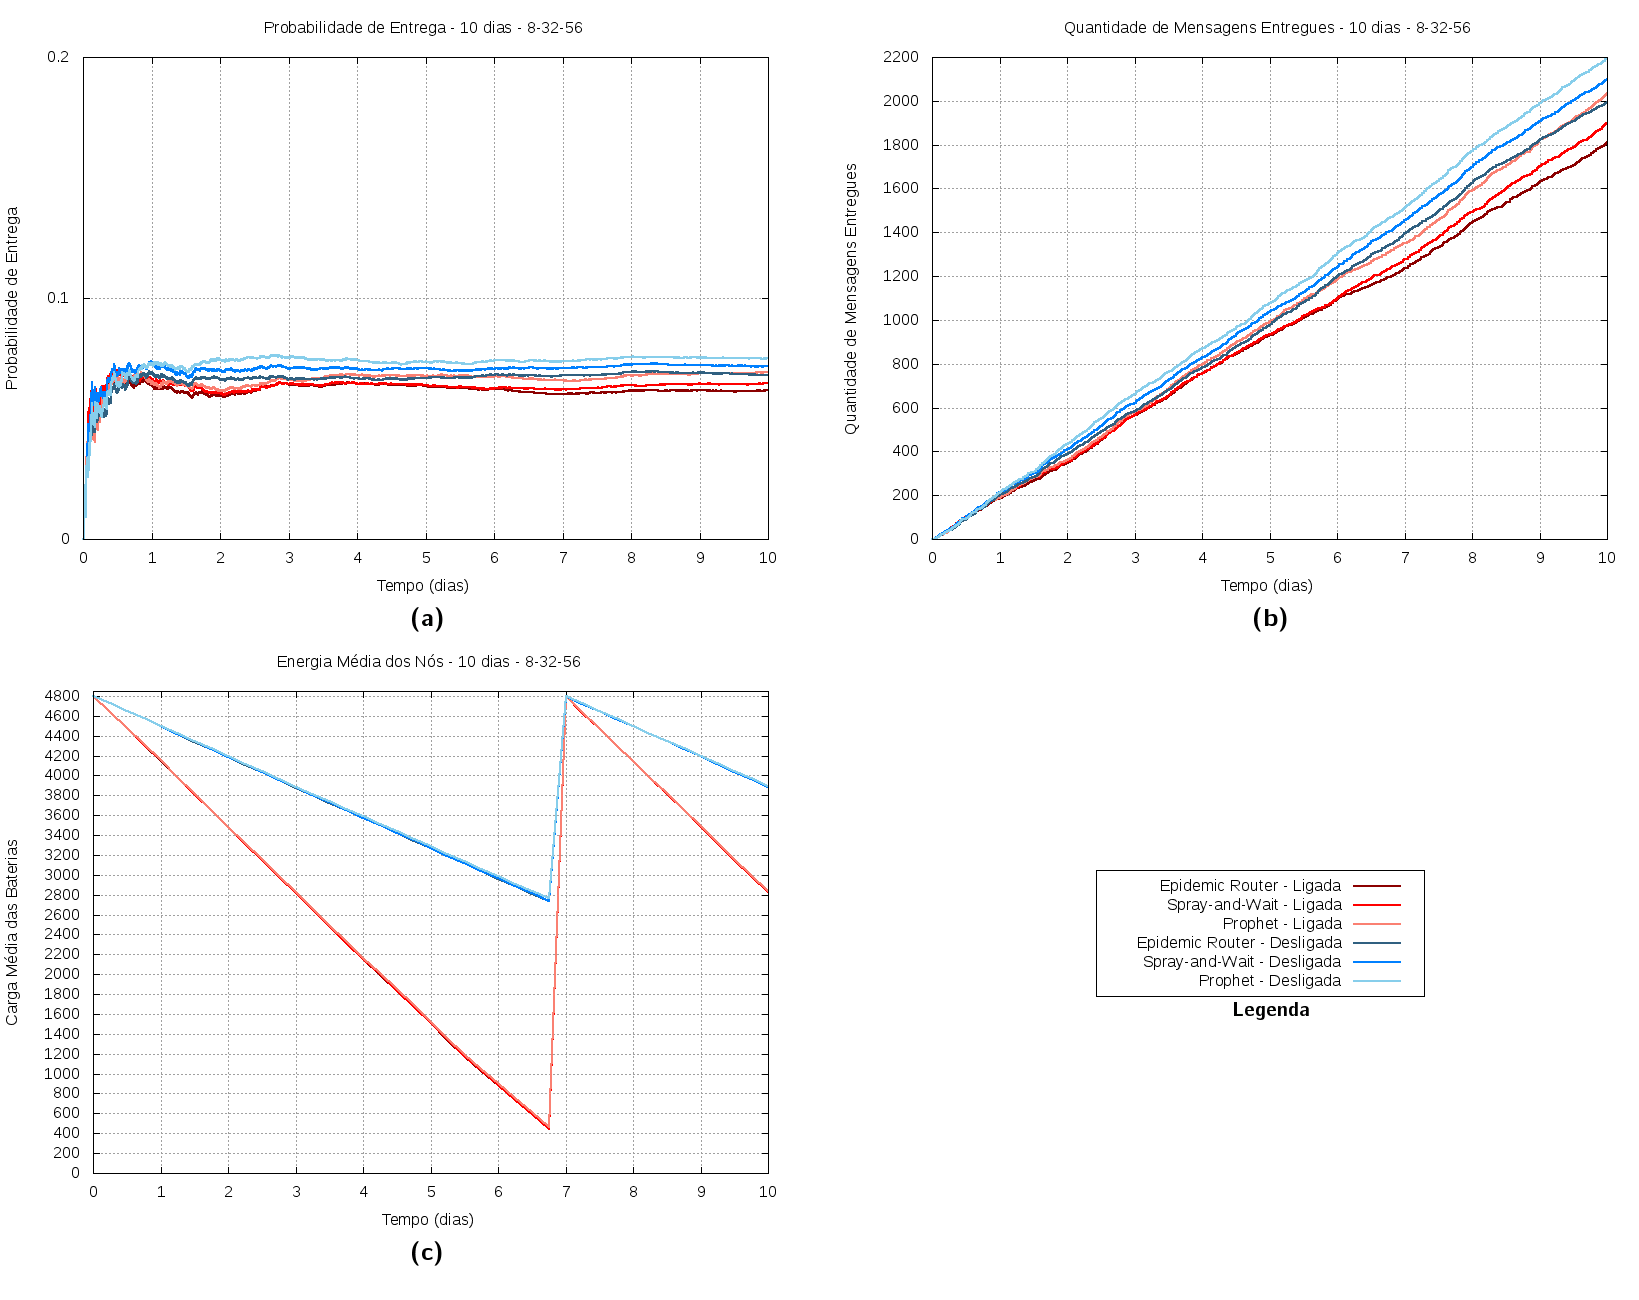
\includegraphics[width=0.8\textwidth]{figuras/cap_5/graficos/8_32_56/MessageDeliveryReport_10_8-32-56_withRecharge_604800.png}
\caption{Resultados de simulações de 10 dias com recarga periódica de sete dias e período de busca de 8, 32 e 56 segundos.}
\label{10dias_8-32-56_comRecarga}
\end{sidewaysfigure}

\begin{sidewaysfigure}
\centering
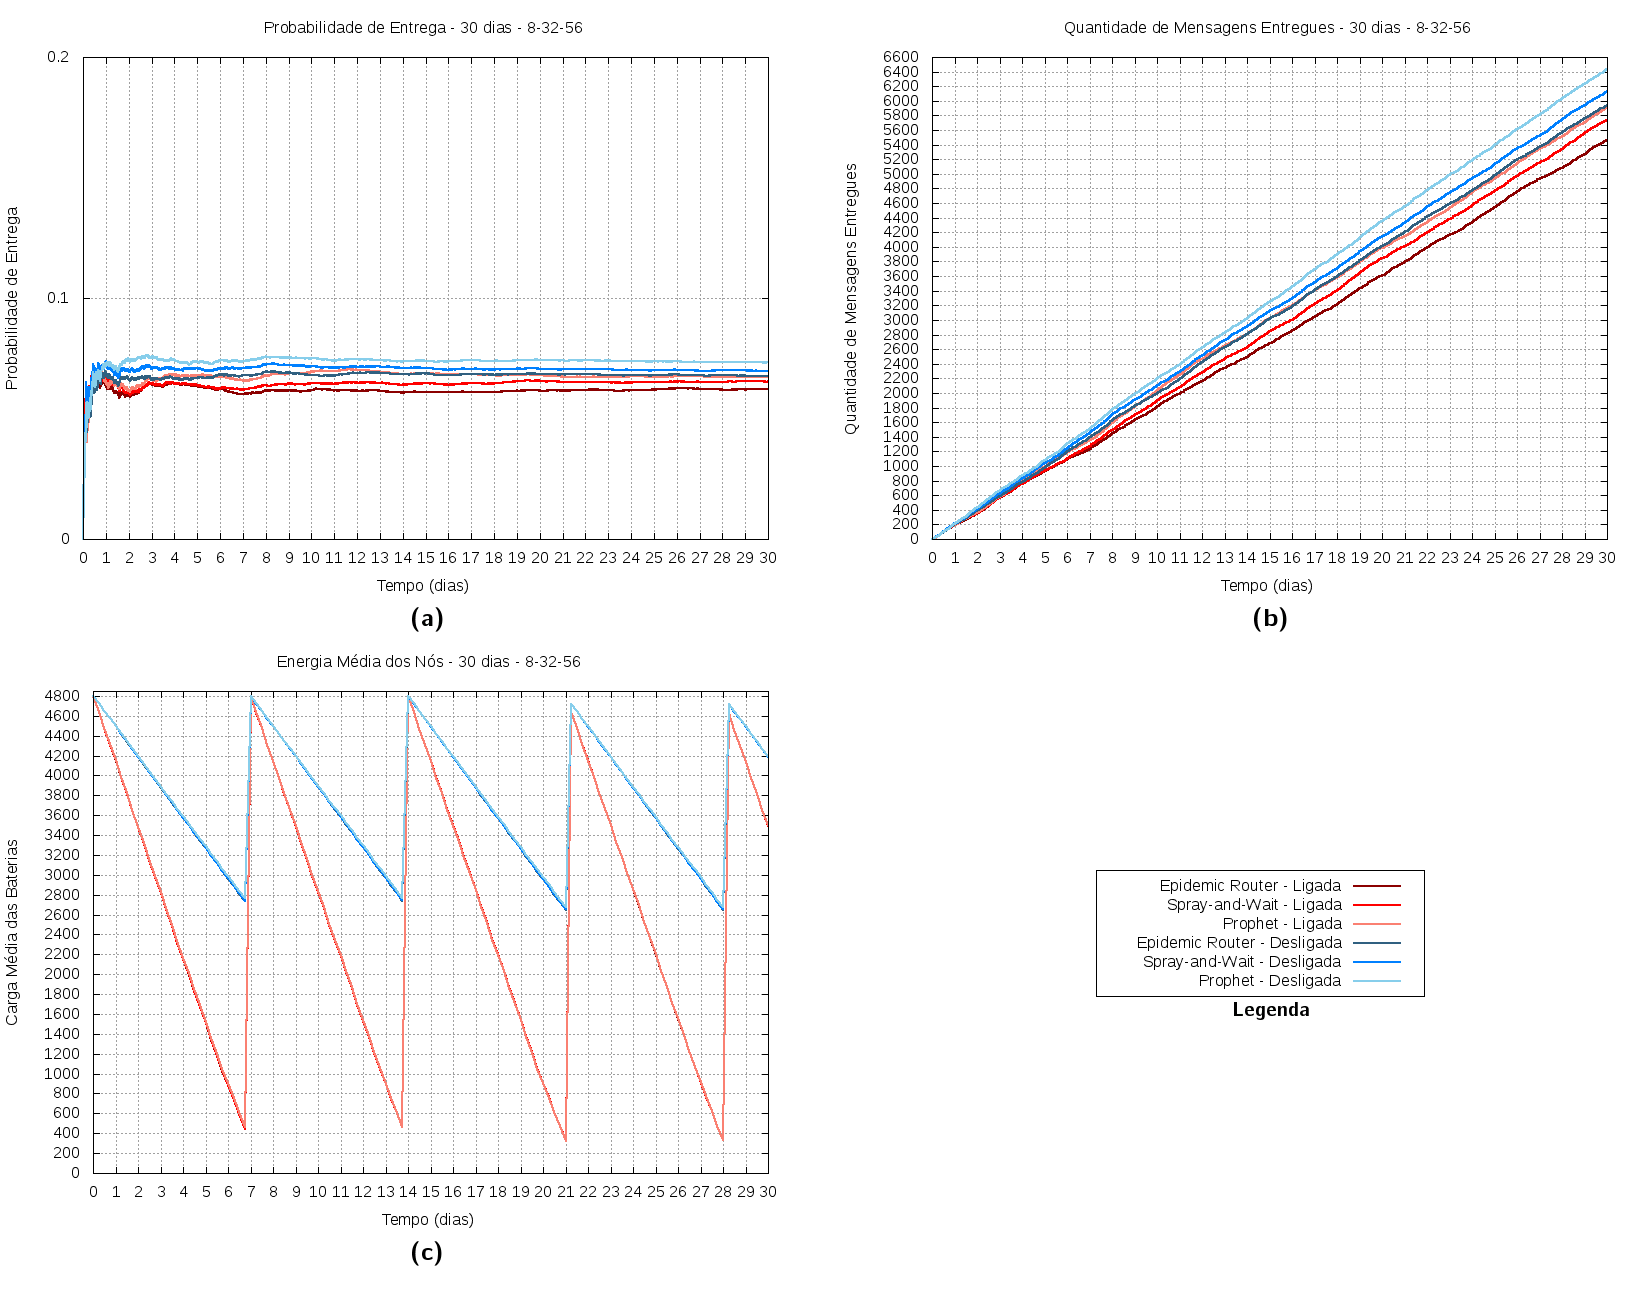
\includegraphics[width=0.8\textwidth]{figuras/cap_5/graficos/8_32_56/MessageDeliveryReport_30_8-32-56_withRecharge_604800.png}
\caption{Resultados de simulações de 30 dias com recarga periódica de sete dias e período de busca de 8, 32 e 56 segundos.}
\label{30dias_8-32-56_comRecarga}
\end{sidewaysfigure}

Quando analisado o consumo de energia, o comportamento dos gráficos \emph{c} das Figuras \ref{10dias_8-32-56_comRecarga} e \ref{30dias_8-32-56_comRecarga} é semelhante, visto que as redes utilizam os mesmos parâmetros de simulação, diferindo apenas na quantidade de tempo considerada. A técnica visivelmente gera um consumo expressivo das baterias que, neste cenário, não é bem aproveitado quando considerada a quantidade de mensagens entregues e a probabilidade de entrega de mensagens.

\subsubsection{Intervalo de Busca de 8, 32 e 32 Segundos}
\label{8-32-32_comRecarga}

O desempenho satisfatório quanto a entrega de mensagens durante o tempo de atividade da rede visto apresentado nos resultados testes da Figura \ref{10dias_8-32-32_semRecarga} pode ser explorado quando a recarga das baterias é considerada, pois a rede encerrou a sua atividade pela escassez de recursos energéticos.

Intuitivamente, pode-se considerar que o ponto ideal de recarga localiza-se no instante de tempo onde as linhas da probabilidade de entrega se cruzam, pois é nesse momento que a técnica começa a apresentar desvantagem em relação a sua não utilização. Tal ponto está no início do quinto dia e este é utilizado como parâmetro na simulação representada pela Figura \ref{10dias_8-32-32_comRecarga_450000} como intervalo de recarga.

\begin{sidewaysfigure}
\centering
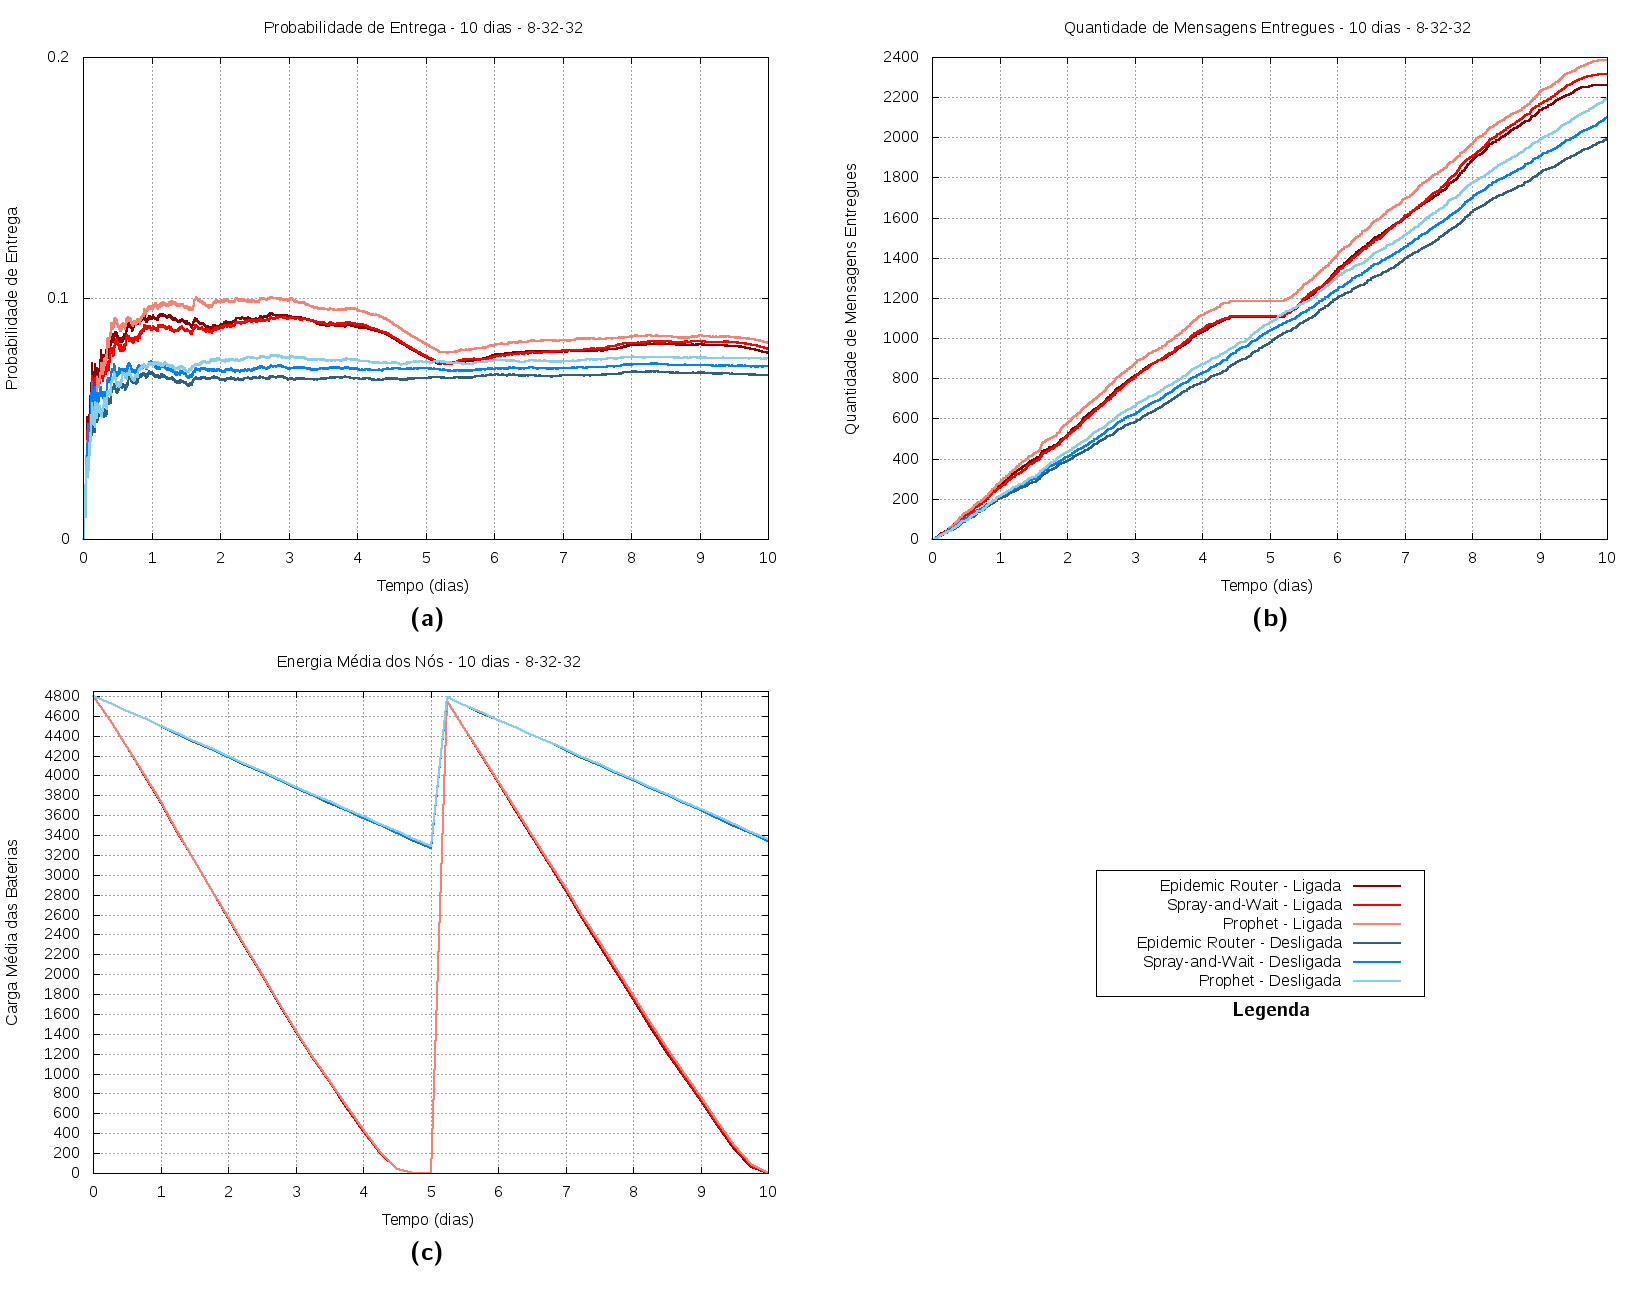
\includegraphics[width=0.8\textwidth]{figuras/cap_5/graficos/8_32_32/MessageDeliveryReport_10_8-32-32_withRecharge_450000.png}
\caption{Resultados de simulações de 10 dias com recarga periódica de cinco dias e período de busca de 8, 32 e 32 segundos.}
\label{10dias_8-32-32_comRecarga_450000}
\end{sidewaysfigure}

Os resultados, entretanto, demonstram que recarregar as baterias no período proposto não é vantajoso. Como pode ser visto no gráfico \emph{c}, a rede interrompe a sua operação por falta de energia por volta da metade do quarto dia, entretanto a recarga das baterias só é realizada 12 horas depois. A inatividade da rede resulta na interrupção da entrega de mensagens, como visto no gráfico \emph{b}, e, consequentemente, na diminuição da probabilidade de entrega, como apresentado no gráfico \emph{a}. Após a recarga das baterias a rede volta a entregar mensagens, porém a probabilidade de entrega não retorna ao valor que estava antes das baterias esgotarem suas cargas.

Recarregar as baterias de cinco em cinco dias não aproveita totalmente o potencial que a técnica possui quanto a entrega de mensagens, pois muitas oportunidades de contato são perdidas durante o período de inatividade da rede. A técnica, no entanto, apresentou um desempenho superior a uma rede que não a utiliza, visto que foi capaz de entregar 2320 mensagens contra 2097 mensagens, ou seja, uma diferença de 223 mensagens a mais. Todos os valores referem-se às médias de mensagens entregues no período simulado.

\newpage
Tendo em vista os resultados da Figura \ref{10dias_8-32-32_comRecarga_450000}, um período de recarga de quatro dias foi proposto e os resultados das simulações são apresentados na Figura \ref{10dias_8-32-32_comRecarga_345600}. Pode ser visto no gráfico \emph{b} da Figura \ref{10dias_8-32-32_comRecarga_345600} que a técnica obteve um melhor aproveitamento quanto a quantidade de mensagens entregues e que, por sua vez, refletiu na probabilidade de entrega que se manteve praticamente constante e acima da rede que não a utiliza após a sua estabilização ao final do terceiro dia.

\begin{sidewaysfigure}
\centering
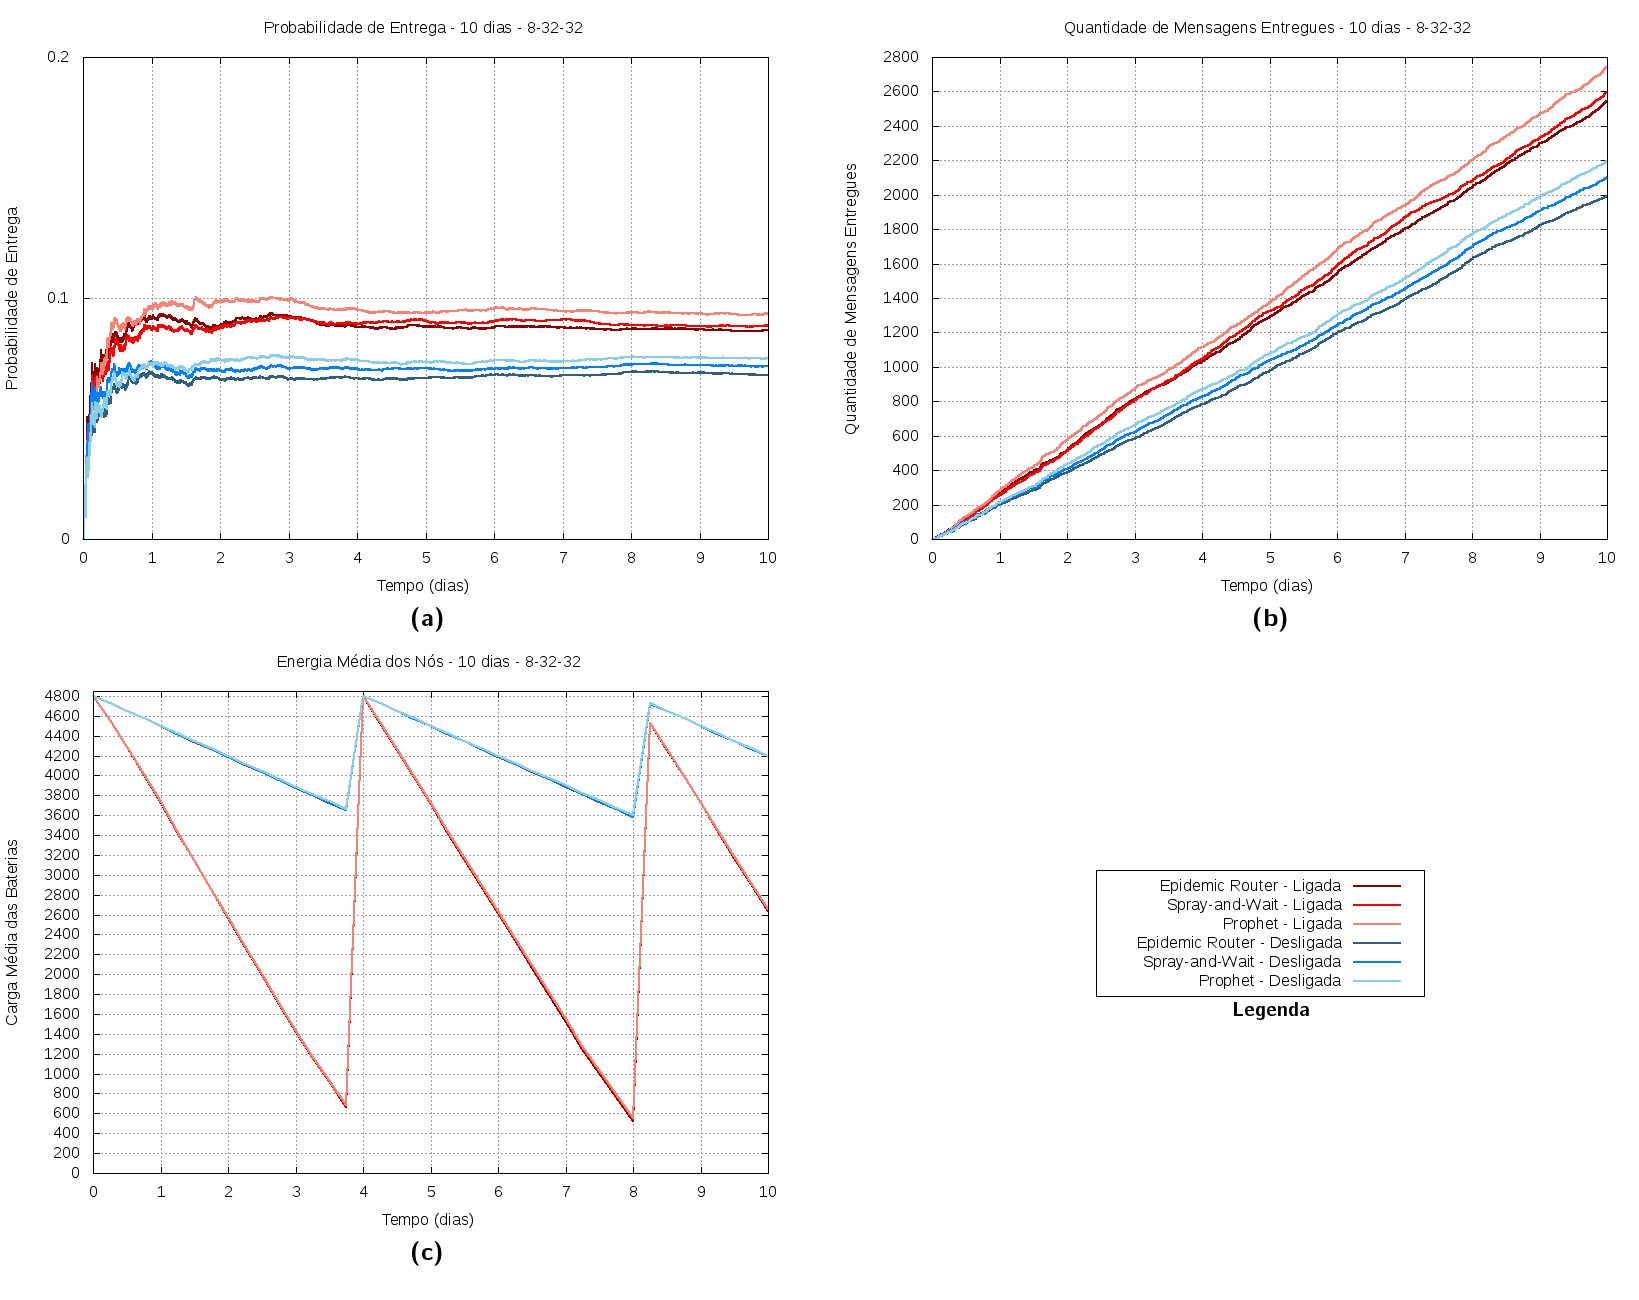
\includegraphics[width=0.8\textwidth]{figuras/cap_5/graficos/8_32_32/MessageDeliveryReport_10_8-32-32_withRecharge_345600.png}
\caption{Resultados de simulações de 10 dias com recarga periódica de quatro dias e período de busca de 8, 32 e 32 segundos.}
\label{10dias_8-32-32_comRecarga_345600}
\end{sidewaysfigure}

Ainda do contexto dos resultados apresentados na Figura \ref{10dias_8-32-32_comRecarga_345600}, a rede que utiliza o intervalo fixo de 32 segundos foi capaz de entregar 2096 mensagens contra 2627 mensagens da rede que utiliza a técnica desenvolvida, ou seja, uma diferença de 531 mensagens. Todos os valores se referem as médias dos resultados observados.

Quando analisada num período de 30 dias, foram obtidos os resultados apresentados na Figura \ref{30dias_8-32-32_comRecarga_345600}, onde é percebido um aumento na diferença de quantidade de mensagens entregues. Em números, a técnica desenvolvida foi capaz de entregar 7832 mensagens contra 6170 mensagens por uma rede com intervalo de busca fixo em 32 segundos. Ou seja, a média de mensagens entregues subiu de 531 para 1662. Novamente, todos os valores referem-se as médias dos resultados observados. A probabilidade de entrega, como consequência do maior número de mensagens entregues, também permaneceu acima de uma rede que não faz uso da técnica desenvolvida.

\begin{sidewaysfigure}
\centering
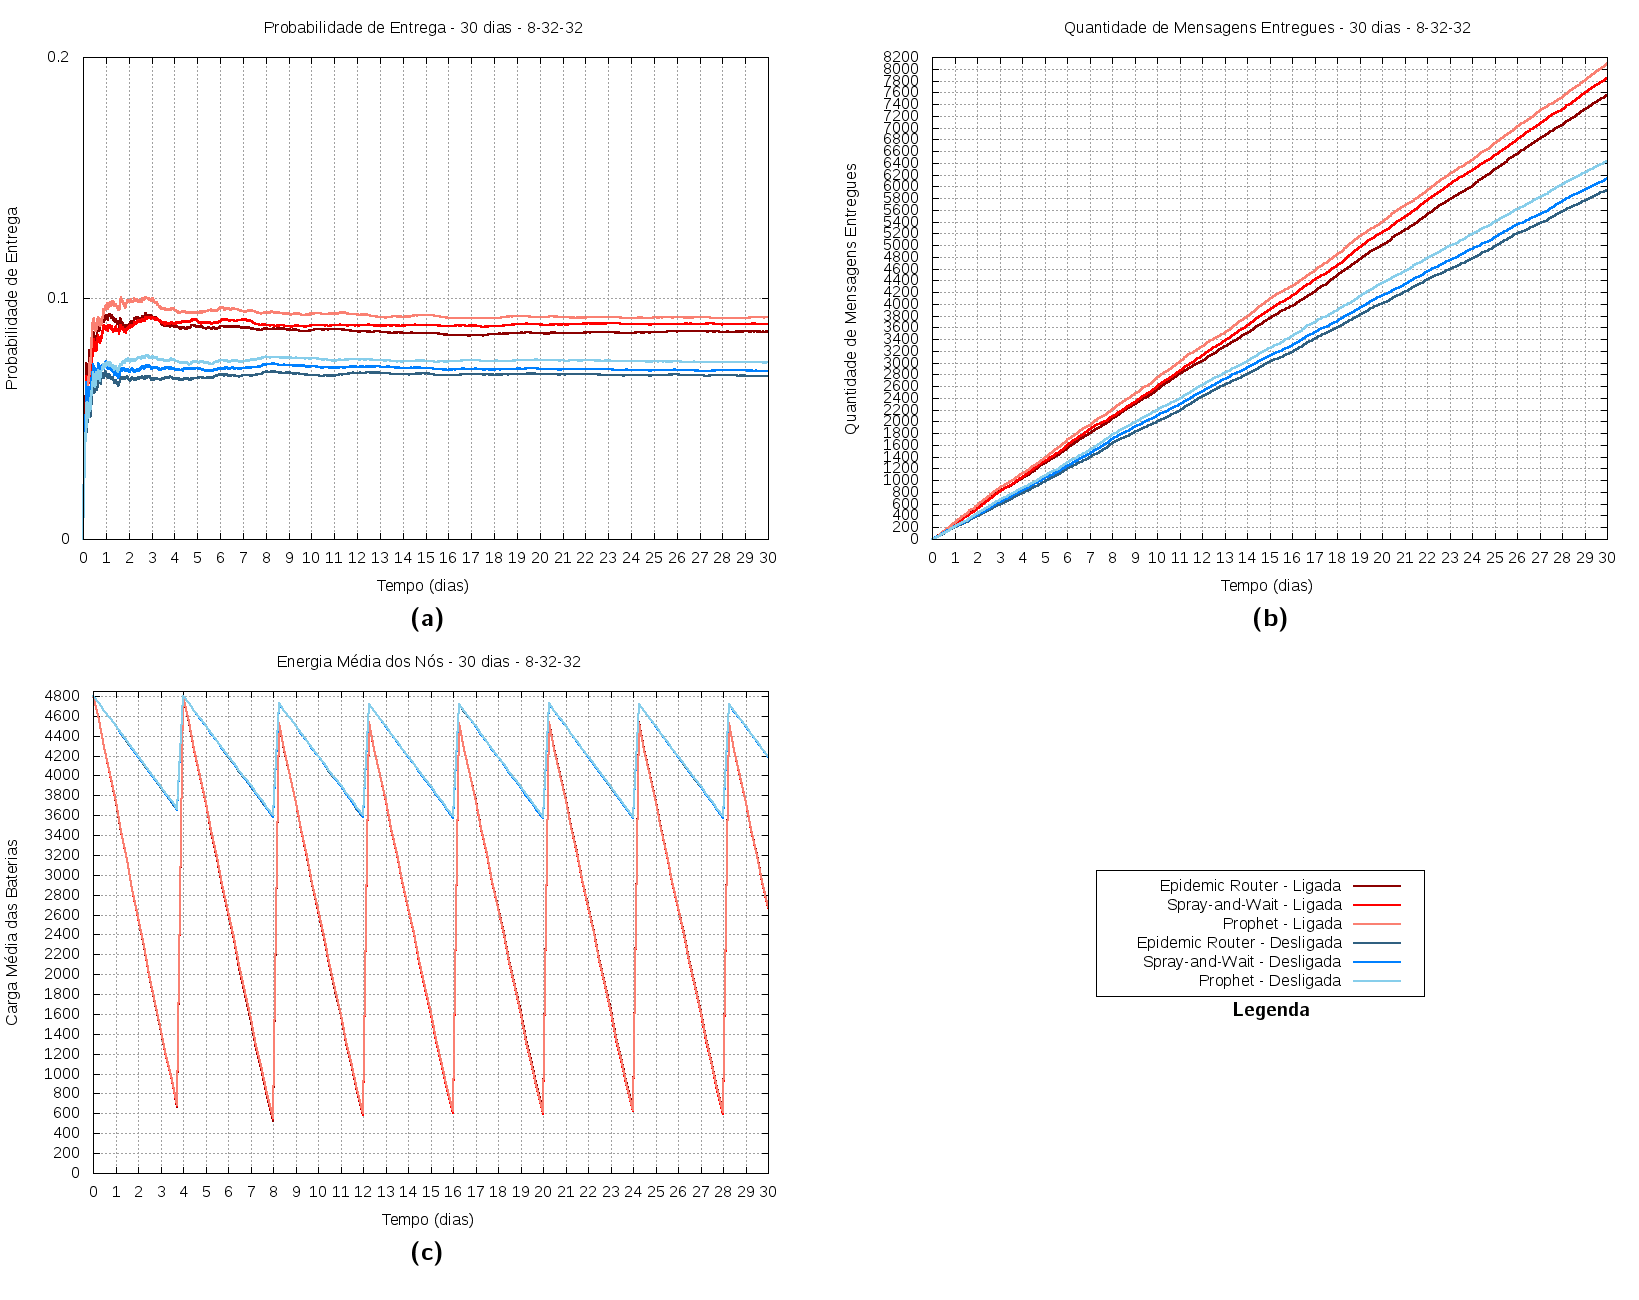
\includegraphics[width=0.8\textwidth]{figuras/cap_5/graficos/8_32_32/MessageDeliveryReport_30_8-32-32_withRecharge_345600.png}
\caption{Resultados de simulações de 30 dias com recarga periódica de quatro dias e período de busca de 8, 32 e 32 segundos.}
\label{30dias_8-32-32_comRecarga_345600}
\end{sidewaysfigure}

\subsubsection{Discussões Sobre o Cenário com Recarga das Baterias}

A ineficiência da técnica quanto ao intervalo de 8, 32 e 56 segundos foi novamente observada, desta vez em um cenário onde a recarga das baterias foi considerada. A quantidade inferior de mensagens entregues e, consequentemente, a menor probabilidade de entrega em relação a sua não utilização torna ineficiente o uso da técnica com os parâmetros definidos, visto que ela não foi capaz de compensar o consumo adicional das baterias em prol da entrega de mensagens.

O intervalo de 8, 32 e 32 segundos, entretanto, apresentou um desempenho melhor quando analisada a probabilidade de entrega e a quantidade de mensagens entregues. Num cenário de simulação de 30 dias, em média, a técnica foi capaz de entregar de 7832 mensagens contra 6170 mensagens entregues por uma rede que baseia-se no período fixo de 32 segundos. A diferença positiva de 1662 mensagens entregues pela técnica é considerável e, quanto maior o tempo de atividade da rede, maior será este valor.

O consumo adicional de energia gerado pela técnica, no caso do intervalo de 8, 32 e 32 segundos, traduziu-se numa maior quantidade de mensagens entregues. Evidenciando assim que tornar inteligente o consumo das baterias não significa, necessariamente, poupá-las.

Discussões sobre o ponto ótimo de recarga devem ser realizadas. Neste trabalho foi evidenciado, por meio dos resultados apresentados nas Figuras \ref{10dias_8-32-32_comRecarga_450000} e \ref{10dias_8-32-32_comRecarga_345600}, que o período de recarga precisa, necessariamente, ser no máximo o tempo de vida da rede implementada para que a técnica tenha melhor aproveitamento quanto a quantidade de mensagens entregues. Isso se deve ao fato de que, caso o período seja maior que o tempo máximo que a rede consegue ficar ativa, os dispositivos irão ficar inativos repetidamente e, como consequência, diversas oportunidades de contato serão perdidas e interrupções na entrega de mensagens serão observadas.


\section{Conclusão do Capítulo}

Neste capítulo foram apresentados os cenários de teste considerados além dos resultados dos testes realizados. Neste trabalho, optou-se por definir os cenários de teste com base no utilizado por \cite{denis_artigo}, pois serviu como uma importante referência dentro literatura de DTNs. Além disso, foram considerados os dois estados principais da técnica, desligada e ligada, com o intuito de avaliar o seu comportamento quando comparada a uma rede que não a utiliza.

Acerca dos resultados, foi apresentado neste capítulo que o desempenho da técnica não é satisfatório quando analisa-se unicamente a economia das baterias. Entretanto, quando a recarga das baterias é considerada, a técnica é capaz de auxiliar no aumento da quantidade de mensagens entregues dependendo do intervalo de busca mínimo, padrão e máximo definidos. Neste trabalho, optou-se por testar apenas dois períodos, 
entretanto a busca por um período ideal é totalmente passível de ser realizada em trabalhos futuros.

Além disso, o aumento do consumo de energia relacionado ao aumento da entrega de mensagens por parte da técnica evidenciou que tornar inteligente o consumo das baterias não, necessariamente, significa economizá-las, mas sim consumí-la de acordo com a situação em que o nó se encontra. Ou seja, gastar em momentos oportunos e poupá-la em momentos não favoráveis.


%capítulo 6 - Conclusão
\chapter{CONCLUSÃO}\label{conc}

A construção deste Trabalho de Conclusão do Curso permitiu ampliar o conhecimento por meio de pesquisas relacionadas à área de Redes Tolerantes a Atrasos e Desconexões, além de ter servido como apoio para a obtenção de conhecimento acerca das tecnologias e ferramentas ligadas à Geolocalização e simulação de protocolos de rede.

Todo o esforço empregado para o desenvolvimento da técnica proposta teve como principal objetivo dinamizar o intervalo de busca ótimo de 32 segundos proposto por \cite{denis_artigo} de forma a melhor aproveitar as oportunidades de contato de acordo com com a probabilidade deles ocorrem em regiões geográficas previamente definidas, sendo de grande valia, este trabalho, para dar continuidade a pesquisas relacionadas ao intervalo entre buscas por dispositivos móveis dentro da área de DTNs.

A partir dos testes realizados no Capítulo \ref{cap:testes}, foi evidenciado que o uso da técnica em ambientes onde não há recarrega as baterias prejudica o desempenho da rede, uma vez que elas se esgotam muito rapidamente devido ao consumo adicional gerado pela técnica, oriundo principalmente pelo uso de dispositivos GPS. A morte da rede se traduz na interrupção da entrega de mensagens e, consequentemente, faz com que a técnica fique em desvantagem quanto a entrega de mensagens e a probabilidade de entrega ao ser comparada a uma rede que não a utiliza.

Em cenários onde a recarga periódica das baterias é possível, entretanto, os resultados mostraram que a utilização da técnica oferece vantagens. Nos testes realizados com o intervalo de busca mínimo de 8, padrão de 32 e máximo de 32 segundos, por exemplo, em 30 dias de simulação, uma média de 7832 mensagens foram entregues com a técnica, contra 6170 mensagens entregues sem ela. Ou seja, uma média de 1632 mensagens a mais entregues quando a técnica foi utilizada. Como consequência da maior quantidade de mensagens entregues, a probabilidade de entrega também se manteve acima de uma rede que utiliza o intervalo fixo de 32 segundos. Vale ressaltar que é considerado o consumo adicional gerado pelos dispositivos de geolocalização.

Conclui-se também que tornar inteligente o consumo das baterias em prol do aumento da quantidade de mensagens entregues e da probabilidade de entrega não, necessariamente, significa economizá-las, mas sim gastar mais em momentos oportunos e economizá-las em momentos desfavoráveis.

Por fim, a técnica é forte candidata a ser utilizada em ambientes onde há a possibilidade de recarga das baterias, desde que estas ocorram antes da interrupção da atividade da rede por falta de energia.

\section{Trabalhos Futuros}

Quanto ao módulo de análise do consumo de energia, existem melhorias que podem ser desenvolvidas com o objetivo de aumentar o realismo do cenário de simulação. A sobrecarga gerada pela técnica na troca e intercalação das tabelas de mapeamento não foi considerada pelo módulo neste trabalho devido a uma limitação do escopo, mas, no futuro, pretende-se analisar o comportamento da rede quando considera-se esses fatores.

As regiões geográficas definidas neste trabalho basearam-se em áreas quadradas com 500 metros de lado. O tamanho dessas regiões influencia diretamente na quantidade de informações que serão armazenadas nas tabelas de mapeamento e, consequentemente, deve ser ajustado de acordo com as limitações existentes nos dispositivos que compõem a rede DTN. Pretende-se então, no futuro, analisar o impacto quanto ao armazenamento dessas tabelas e o quanto ele influencia positivamente e negativamente no aproveitamento das oportunidades de contato pela técnica desenvolvida. 

Além disso, planeja-se também estudar a existência de um período mínimo, máximo e padrão de busca ideal, de forma a aproveitar ainda mais as oportunidades de contato e, como consequência, aumentar também a quantidade de mensagens entregues e a probabilidade de entrega de mensagens.

No futuro, planeja-se abordar essas e outras questões que possam contribuir para um melhor aproveitamento dos recursos nas Redes Tolerantes a Atrasos e Desconexões.


%==============================================================================
%				  BIBLIOGRAFIA / REFERÊNCIAS
%==============================================================================
\bibliography{bibliografia}
\bibliographystyle{abnt-alf}

%Fim do documento
\end{document}